\documentclass[a4paper]{article}

\usepackage{array}
\usepackage[
    style=apa, 
    backend=biber, 
    sorting=none
]{biblatex}
\usepackage{booktabs}
\usepackage{multirow}
\usepackage{graphicx}
\usepackage{enumitem}
\usepackage{geometry}
\usepackage{sectsty}
\usepackage{indentfirst}
\usepackage{times}
\usepackage{listings}
\usepackage{longtable}
\usepackage{array}
\usepackage{caption}
\usepackage{setspace}
\usepackage[colorlinks=true,linkcolor=black,anchorcolor=black,citecolor=black,filecolor=black,menucolor=black,runcolor=black,urlcolor=black]{hyperref}
\usepackage{chngcntr}
\usepackage{makecell}
\usepackage{pdfpages}
\usepackage{tocloft}

\setlist{
  listparindent=\parindent,
  parsep=0pt,
}
\counterwithin{figure}{section}
\counterwithin{table}{section}
\newcounter{counttable}

% code block style
% -- Defining colors:
\definecolor{codegreen}{rgb}{0,0.6,0}
\definecolor{codegray}{rgb}{0.5,0.5,0.5}
\definecolor{codepurple}{rgb}{0.58,0,0.82}
\definecolor{backcolour}{rgb}{0.95,0.95,0.92}% Definig a custom style:
\definecolor{Black}{rgb}{1,1,1}
\lstdefinestyle{mystyle}{
    backgroundcolor=\color{backcolour},   
    keywordstyle=\color{codegreen},
    numberstyle=\tiny\color{codegray},
    stringstyle=\color{codepurple},
    basicstyle=\ttfamily\footnotesize\bfseries,
    breakatwhitespace=false,         
    breaklines=true,                 
    captionpos=t,                    
    keepspaces=true,                 
    numbers=left,                    
    numbersep=5pt,                  
    showspaces=false,                
    showstringspaces=false,
    showtabs=false,                  
    tabsize=2
}% -- Setting up the custom style:
\lstset{style=mystyle}

\sectionfont{\centering}
\addbibresource{citation/citation.bib}
\addbibresource{citation/aldih.bib}
\addbibresource{citation/chandra.bib}
\graphicspath{{./images/}, {./diagram}}
\geometry{a4paper, top=4.0cm, bottom=3.0cm,
          left=4.0cm, includehead, includefoot}
\renewcommand\contentsname{Daftar Isi}
\renewcommand\listfigurename{Daftar Gambar}
\renewcommand\listtablename{Daftar Tabel}
\emergencystretch=2em

% table lampiran
\newcommand{\listappendicesname}{Daftar Lampiran}
\newlistof{appendices}{apc}{\listappendicesname}
\newcommand{\appendices}[1]{\addcontentsline{apc}{appendices}{#1}}

% bab command
\newcommand{\bab}[1]{%
    \addtocounter{section}{1}%
    \setcounter{subsection}{0}
    \setcounter{subsubsection}{0}
    \setcounter{figure}{0}
    \setcounter{table}{0}
    \section*{#1}%
    \addcontentsline{toc}{section}{\protect\numberline{}#1}%
}

\newcommand{\subbab}[1]{%
    \subsection{#1}%
    \setcounter{figure}{0}
    \setcounter{table}{0}
    % \addcontentsline{toc}{subsection}{\protect\numberline{}#1}%
}

\newcommand{\subsubbab}[1]{%
    \subsubsection{#1}%
    % \addcontentsline{toc}{subsubsection}{\protect\numberline{}#1}%
}

\begin{document}
\setstretch{1.5}
\pagenumbering{roman}
\date{}
\title{Shumishumi - Pasar Daring untuk Hobi dengan Penyaringan Tingkat Minat dan Sistem Rekomendasi Menggunakan Implementasi Knowledge Graph}
\clearpage\maketitle
\addcontentsline{toc}{section}{\protect\numberline{}Halaman Sampul}
\setstretch{1.5}
\vspace{4em}%
\begin{center}
    \textbf{Oleh}\\%
    \vspace{0.10cm}%
    2301862632 - Aldih Suhandi\\%
    2301872596 - Chandra Wijaya\\%
    2301867324 - Ibrahim Seto Aditama\\%
    Kelas/Kelompok : LB01/016
\end{center}
\thispagestyle{empty}
\begin{figure}[h]
    \centering
    
\includegraphics[width=8cm,height=4cm]{logo_binus.png}\\
    \textbf{School of Computer Science\\
    Universitas Bina Nusantara\\
    Jakarta\\
    2023}
\end{figure}

\newpage
\addcontentsline{toc}{section}{\protect\numberline{}Halaman Judul}

\includepdf[pages=1]{pdf/thesis-title.pdf}

\newpage
\addcontentsline{toc}{section}{\protect\numberline{}Halaman Pernyataan Orisinalitas}

\includepdf[pages=1]{pdf/Halaman Originalitas.pdf}

\newpage
\addcontentsline{toc}{section}{\protect\numberline{}Abstrak}
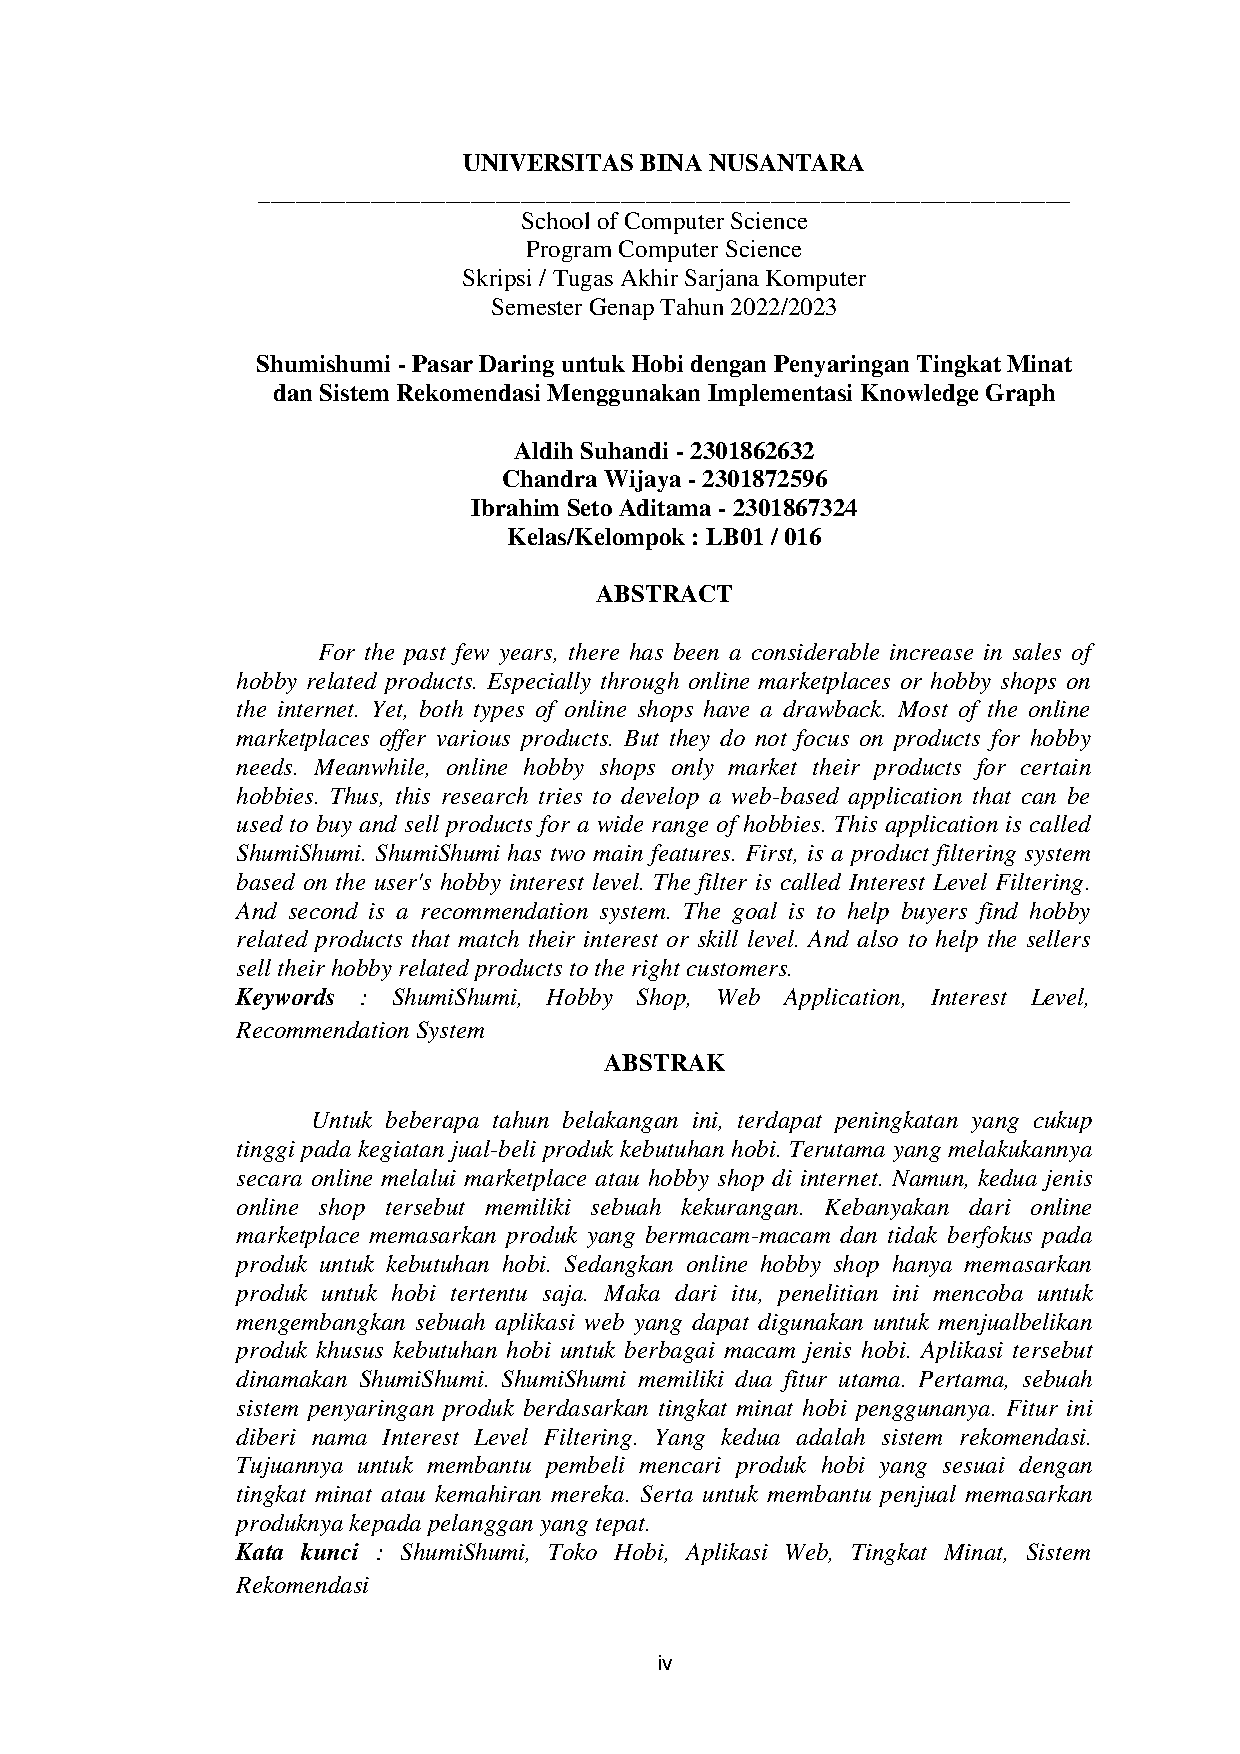
\includepdf[pages=1]{pdf/Abstrak.pdf}

\newpage
\addcontentsline{toc}{section}{\protect\numberline{}Kata Pengantar}
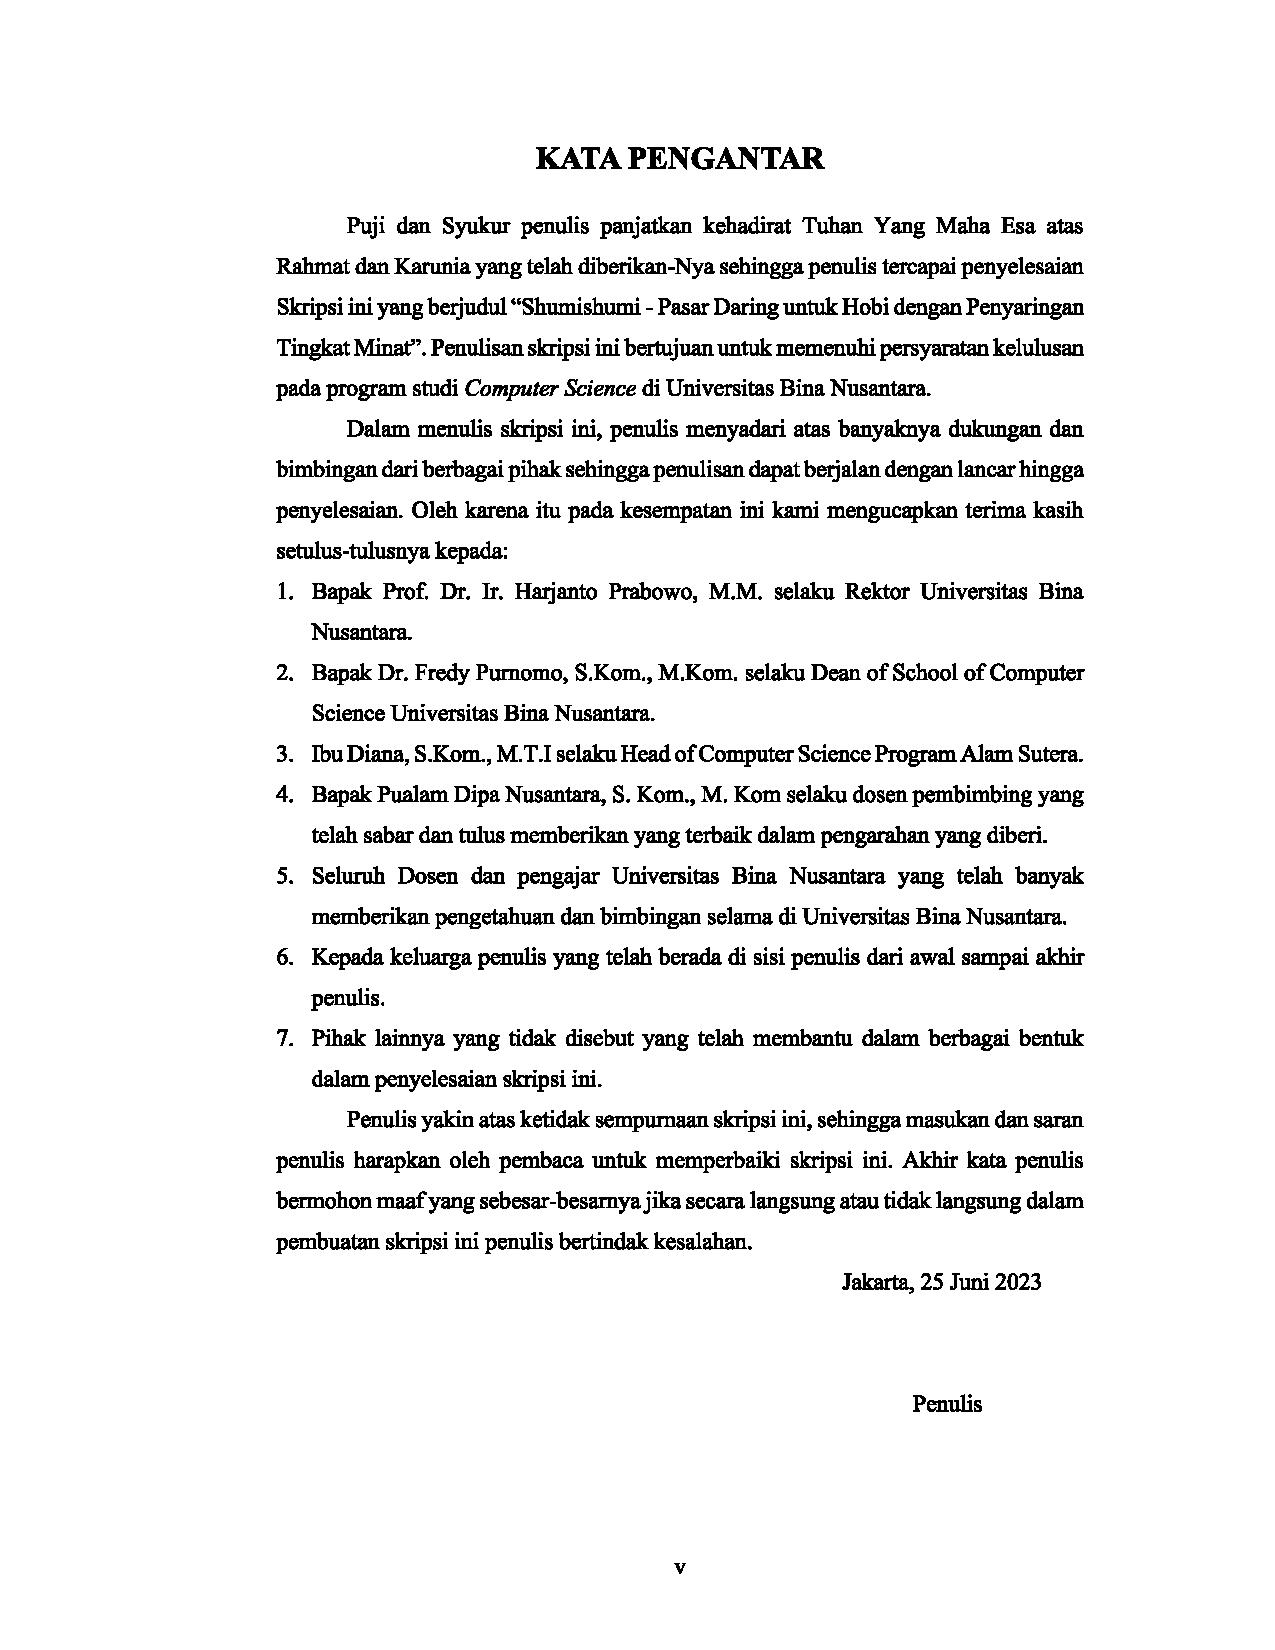
\includepdf[pages=1]{pdf/Kata_Pengantar_3_Doang.pdf}

\newpage
\addcontentsline{toc}{section}{\protect\numberline{}Daftar Isi}
\tableofcontents

\newpage
\addcontentsline{toc}{section}{\protect\numberline{}Daftar Tabel}
\listoftables

\newpage
\addcontentsline{toc}{section}{\protect\numberline{}Daftar Gambar}
\listoffigures

\newpage
\addcontentsline{toc}{section}{\protect\numberline{}Daftar Lampiran}
\listofappendices

\newpage
\pagenumbering{arabic}
\bab{Bab 1. Pendahuluan}

\subbab{Latar Belakang}

Hobi dapat diartikan sebagai suatu aktivitas yang dilakukan dalam waktu luang dengan tujuan untuk mendapatkan rasa kebahagiaan. Hobi ini juga dapat menjadi distraksi dari rasa gelisah yang dimiliki atau dialami oleh seseorang. Hobi juga dapat memberi rasa tujuan hidup kepada seseorang, terutama ketika hobi tersebut dapat dilakukan bersama-sama dengan sebuah kelompok yang memiliki minat hobi yang sejenis\autocite{zaidi2022passion}.

Tidak semua hobi dapat dilakukan dengan mudahnya tanpa memerlukan barang-barang tertentu yang khusus digunakan untuk menjalankan aktivitas hobi tersebut. Seperti contoh, bagi seseorang yang memiliki hobi memancing, orang tersebut harus memiliki alat pemancing ikan untuk bisa melakukan aktivitas tersebut. Contoh lainnya adalah orang-orang yang memiliki hobi bermain bulu tangkis (\textit{badminton}), mereka harus mempunyai raket \textit{badminton} terlebih dahulu agar bisa menjalankan hobi tersebut. Maka dari itu, barang-barang tersebut perlu dicari dan didapatkan terlebih dahulu. Caranya adalah dengan mendatangi toko yang menjual barang-barang tersebut atau membeli barang tersebut secara \textit{online} melalui \textbf{internet}.

Internet merupakan salah satu hasil dari perkembangan teknologi yang memiliki dampak cukup tinggi kepada kehidupan masyarakat. Dimana di Indonesia sendiri saja, internet mendapatkan peningkatan popularitas yang cukup drastis. Hal ini dapat dilihat dengan menganalisa peningkatan jumlah pengguna internet tersebut di setiap tahunnya. Menurut survey yang diadakan oleh Asosiasi Penyelenggara Jasa Internet Indonesia (APJII) pada tahun 2017, perkembangan jumlah pengguna internet di Indonesia dari tahun 2016 ke tahun 2017 sendiri memiliki peningkatan sebanyak 10.56 juta pengguna, yakni dari 132.7 juta pengguna di tahun 2016 hingga 143.26 juta pengguna pada tahun 2017\autocite{indonesia2017infografis}.

Dari berbagai macam kegiatan \textit{online} yang dilakukan di internet, aktivitas usaha jual beli barang merupakan salah satu kegiatan yang cukup populer dilakukan di Internet. Dimulai dari yang melakukannya melalui percakapan daring secara \textit{text}/\textit{chatting} maupun yang melalui suatu pasar jual-beli barang daring seperti \textit{e-commerce}. Dimana di Indonesia sendiri berdasarkan survei yang dilakukan oleh Asosiasi Penyelenggara Jasa Internet Indonesia (APJII), proses pembelian barang \textit{online} mencakupi sebesar 32.19\% pada layanan yang diakses ketika menggunakan internet dan sebesar 8.12\% untuk proses penjualan barangnya\autocite{indonesia2017infografis}. \textit{Platform} yang digunakan untuk mempermudah usaha kegiatan jual-beli barang biasanya dilengkapi dengan fitur pencarian/\textit{searching} yang cukup cepat, dimana barang dapat dicari dan ditemukan melalui pencarian namanya ataupun menelusuri kategori dari barang tersebut. Kegiatan jual-beli barang ini mencakupi kebutuhan bahan baku hingga kebutuhan-kebutuhan tambahan lainnya.

Biasanya, kegiatan jual-beli secara \textit{online} berlangsung pada sebuah sarana aplikasi yang bernama \textit{Web Application} atau aplikasi web. Aplikasi web itu sendiri adalah sebuah program aplikasi yang di simpan di sebuah \textit{remote server} dan dapat diakses dengan \textit{web browser} melalui internet\autocite{what-is-web-app}. Pada umumnya, barang-barang kebutuhan hobi diperjualbelikan di dalam \textit{e-commerce} atau sebuah \textit{online marketplace}. Di sana, barang kebutuhan hobi dijual bersamaan dengan barang-barang lain yang tidak berhubungan sama sekali dengan suatu hobi. Adapun barang kebutuhan hobi dijual ke sebuah \textit{online marketplace} yang hanya terfokus kepada hobi tertentu saja. \textit{Online marketplace} ini biasa disebut dengan istilah \textit{hobby shop}.

Alasan utama mengapa penelitian ini memilih topik yang berfokus pada kegiatan jual-beli barang kebutuhan hobi adalah dikarenakannya tingginya peningkatan kegiatan jual-beli di pasar kebutuhan barang hobi semenjak pandemi COVID-19 kemarin. Pandemi COVID-19 yang melanda dunia selama kurang lebih dua setengah tahun lamanya itu, membuat banyak orang mengalamai kebosanan dikarenakan adanya \textit{lockdown} dan aturan-aturan \textit{social distancing} ketat yang membuat aktivitas masyarakat menjadi sangat terbatas\autocite{boredom-in-covid-19-pandemic}. Semenjak itulah, banyak orang yang kembali menjalankan kegiatan hobi lama mereka atau bahkan mencari kegiatan lain yang dapat dijadikan hobi baru untuk mengisi waktu luang mereka di masa pandemi tersebut. Hal ini mengakibatkan pasar yang berfokus pada bidang jual beli barang kebutuhan hobi meningkat drastis.

Contohnya dapat dilihat dari salah satu rantai ritel \textit{superstore} yang bergerak di bidang hobi di segi seni dan kerajinan dari Inggris yang bernama Hobbycraft. Mereka melaporkan bahwa pada tahun dimana pandemi COVID-19 sedang merajalela, mereka kedatangan banyak pengguna baru yang berjumlah kurang lebih sebanyak 1.3 juta akun, yang sebagian besarnya adalah para pengguna dari kaum \textit{millenial}\autocite{hobbycraft-fast-online-growth}. Bukti lainnya juga dapat dilihat dari salah satu \textit{e-commerce} terbesar di Indonesia yakni Tokopedia yang melaporkan bahwa hasil penjualan dari transaksi barang-barang yang berhubungan dengan kebutuhan hobi meningkat drastis di masa pandemi COVID-19. Mulai dari hobi olahraga, membaca buku, seni hingga memasak\autocite{tokped-hobbies-goods-sales-increased}.

Alasan lain mengapa topik ini dipilih adalah karena kurangnya jumlah \textit{online hobby shop} yang menjual barang kebutuhan untuk berbagai macam hobi. Kebanyakan dari \textit{hobby shop} yang ada (terutama di Indonesia) hanya berfokus pada satu hobi yang spesifik saja. Salah satu yang cukup terkenal adalah Kyou Hobby Shop atau biasa disebut sebagai KyouID. KyouID merupakan sebuah \textit{hobby shop} yang menjual berbagai jenis produk khusus untuk orang-orang yang hobi mengoleksi produk atau \textit{merchandise} yang berhubungan erat dengan kebudayaan \textit{anime} dari Jepang. Contoh produk yang mereka jual dapat berupa \textit{figurine}/miniatur karakter, stiker dari sebuah karakter, poster seni dan berbagai macam \textit{merchandise} lainnya yang berhubungan dengan satu hobi tersebut.

Maka dari itu, penelitian ini mengusulkan untuk membuat sebuah aplikasi berbasis web yang lebih terfokus ke arah produk-produk kebutuhan hobi dibandingkan dengan \textit{e-commerce} atau \textit{marketplace}. Namun, cakupan hobi untuk aplikasi web ini lebih terfokus ke arah kebutuhan hobi yang lebih luas. Aplikasi web ini mencakupi berbagai macam jenis hobi yang lebih banyak apabila dibandingkan dengan \textit{hobby shop} yang hanya terfokus pada satu jenis hobi saja. Para pengguna dapat mencari dan memilih berbagai macam produk untuk hobi yang berbeda-beda.

Ada beberapa alasan mengapa proyek ini lebih memilih untuk mengembangkan aplikasinya dalam bentuk web. Pertama, aplikasi berbasis web tidak perlu di \textit{install} satu per satu pada tiap \textit{device} dan lebih mudah untuk diakses, karena aplikasi web dapat diakses menggunakan \textit{deivce} apapun selama \textit{device} tersebut mempunyai \textit{web browser} dan koneksi internet. Kedua, aplikasi web tidak bergantung terhadap \textit{platform} apa aplikasi tersebut akan berjalan, karena semuanya dapat diakses melalui \textit{web browser}. Alasan terakhir yang tidak kalah pentingnya, para pengguna tidak perlu pusing-pusing memperbarui aplikasi web yang mereka gunakan secara manual, karena semua pengguna yang mengakses web tersebut pasti akan mendapatkan versi aplikasi web yang terbaru. Proses pembaruan atau peningkatan sistem pada aplikasi web hanya dilakukan pada bagian \textit{server} saja.

Terkadang muncul suatu permasalahan saat ingin memulai hobi baru, yakni kebingungan atau merasa ragu untuk mencari produk yang cocok sebagai titik mulai untuk menjalankan hobi tersebut. Begitu juga dengan para pengguna yang sudah berpengalaman pada hobi tertentu. Terkadang, mereka juga mengalami kesulitan untuk mencari suatu produk yang dapat mendukung kegiatan hobi mereka yang cukup ekstrim atau yang dapat mendukung kegiatan hobi mereka dalam jangka waktu yang lama. Seperti contoh, seseorang yang hobi bersepeda di pegunungan membutuhkan sebuah sepeda yang kokoh dan aman untuk melewati rintangan yang cukup berat di wilayah pegunungan tersebut. Untuk itu, penelitian ini melakukan sebuah survei untuk mengumpulkan pendapat dari para calon pengguna mengenai tingkat kesulitan untuk mendapatkan barang-barang hobi yang diinginkan. Sebagai salah satu bukti dari survei yang diadakan, untuk pertanyaan \textit{"Apakah mencari hobi baru itu sangat sulit?"}, sebanyak 73.2\% dari 123 responden yang ada menjawab \textit{"Iya"}. Untuk itu, aplikasi ini akan mengimplementasikan dua fitur yang dapat membantu para pengguna mencari barang-barang kebutuhan hobi mereka.

% Dari sembilan pertanyaan, ada empat pertanyaan di dalam survei yang menanyakan tingkat kesulitan untuk mencari barang kebutuhan hobi (dimulai dari yang ingin menjalankan hobi baru ataupun yang sudah mendalaminya sejak lama). Empat pertanyaan tersebut adalah sebagai berikut, \textit{"Apakah mencari hobi baru itu sangat sulit?"}. Dari total 123 responden yang menjawab survei tersebut, sebanyak 90 responden atau kurang lebih sebanyak 73.2\% nya menjawab \textit{"Iya"}. Begitu juga untuk pertanyaan selanjutnya, yakni \textit{"Pernahkah anda takut mengambil hobi baru karena tidak tau mulai dari mana?"}, sebanyak 72.4\% dari total responden menjawab \textit{"Iya}. Lalu, pada pertanyaan selanjutnya, \textit{"Pernahkah anda saat memasuki suatu hobi baru bingung, apa saja barang yang perlu dibeli?"}, ada sebanyak 77 responden (62.6\%) menjawab \textit{"Iya"}. Terakhir, \textit{"Apakah anda pernah mengalami kesulitan saat mencari barang yang mau dibeli untuk hobi yang anda sudah dalami?"}, sebanyak 63 responden (51.2\%) menjawab \textit{"Iya"}. Dapat dilihat bahwa perbandingan antara responden yang merasa kesulitan lebih tinggi dibandingkan dengan yang tidak. Untuk itu, aplikasi ini akan mengimplementasikan dua fitur yang dapat digunakan untuk membantu para pengguna mencari barang-barang kebutuhan hobi mereka.

Salah satu fitur tersebut adalah sebuah dua penilaian tingkat peminatan pada suatu barang kebutuhan hobi sebagai sebuah sistem saring tambahan untuk mencari barang tersebut yang diberi nama \textit{Interest Level Filtering}. Penilaian tersebut diberikan oleh penjual barang tersebut dan nantinya juga dapat diberi oleh pembeli sebagai validasi apakah penilaian yang diberikan oleh penjual tersebut sesuai dengan tingkat minat hobinya atau tidak. Fitur ini dibuat dengan tujuan untuk membantu meningkatkan keyakinan pengguna untuk memilih barang kebutuhan hobi yang sesuai dengan hobi yang dilakukannya, dari yang ingin memulai suatu hobi baru maupun yang ingin mencari barang-barang kebutuhan hobi yang sudah bertingkat antusias atau yang sudah berpengalaman.

% Contoh kasus penggunaan fitur \textit{Interest Level} tersebut adalah seperti berikut, misal untuk hobi bermain gitar. Apabila seorang pengguna baru saja menjalani hobi tersebut atau baru saja belajar bermain gitar, tentunya gitar yang cocok untuk memulai belajar adalah sebuah gitar akustik biasa. Maka dari itu, untuk sebuah produk berupa gitar akustik biasa ('biasa' disini berarti yang berstandar rata-rata atau bukan yang bermerek terkenal dan mahal) akan diberikan penilaian setara dengan "\textit{Beginner}" atau "Pemula" oleh penjual dari barang tersebut. Dan penilaian dari penjual tersebut dapat di nilai kembali oleh pembeli setelah membeli produk tersebut. Penilaian dari pembeli itu dapat digunakan sebagai validasi apakah penilaian tersebut cocok dengan barang yang dijualnya, dan begitu seterusnya untuk produk-produk kebutuhan hobi lainnya.

Fitur lain yang akan dikembangkan pada penelitian ini selain dari fitur \textit{Interest Level} diatas adalah sebuah sistem rekomendasi (\textit{Recommendation System}).Sistem rekomendasi ini akan diimplementasikan pada halaman utama aplikasi web ini. Sistem rekomendasi inilah yang akan membantu memberikan saran kepada pengguna terhadap produk-produk yang paling relevan bagi pengguna tersebut. Sistem rekomendasi ini bekerja berdasarkan jenis-jenis barang kebutuhan hobi apa saja yang telah pengguna tersebut cari atau lihat selama menggunakan aplikasi web ini.

Selain dari kedua fitur yang telah dipaparkan diatas, aplikasi berbasis web ini juga mempunyai beberapa fitur pendukung tambahan layaknya sebuah pasar daring (\textit{online marketplace}) pada umumnya. Seperti, tempat untuk berdiskusi/berkomentar mengenai produk tersebut, fitur pembayaran dan fitur ulasan produk.

Tentunya aplikasi \textit{online marketplace} seperti yang dikerjakan pada penelitian ini bukanlah yang pertama kali dibuat atau dikembangkan. Ada beberapa penelitian terdahulu yang juga telah mencoba dan/atau berhasil membuat aplikasi berjenis \textit{marketplace} dengan fitur dan tujuannya yang berbeda antara satu dengan yang lain. Beberapa aplikasi \textit{marketplace} sejenis tersebut dapat dibandingkan dengan aplikasi yang akan dikerjakan pada penelitian ini. Seperti aplikasi pada penelitian yang dilakukan oleh Heru Nugroho dengan rekan-rekannya yaitu sebuah aplikasi \textit{marketplace} berbasis \textit{mobile} yang menjual belikan produk-produk agrikultur. Aplikasi tersebut bertujuan untuk mempermudah para petani atau pekebun untuk menjual belikan produk agrikultur mereka ke masyarakat umum\autocite{agriculture-marketplace}. Selain dari sektor agrikultur, terdapat juga penelitian yang membuat aplikasi sejenis, namun pada sektor perikanan. Yaitu, penelitian yang dilakukan oleh Mohammad Nazrul bersama dengan rekan-rekannya yang membuat aplikasi \textit{marketplace} berbasis \textit{mobile} yang menjual belikan ikan\autocite{fishes-marketplace}. Lalu, pada ruang lingkup yang sama, ada sebuah penelitian yang dilakukan oleh Dwi bersama dengan rekan-rekannya yang membuat aplikasi jual beli ikan menggunakan metode \textit{SMS Gateway}\autocite{c2c-fish-marketplace}. Selanjutnya, penelitian yang dilakukan oleh N F Rozi dan rekan-rekannya dengan membuat aplikasi berbasis web bernama \textbf{LIDI} yang ditujukkan sebagai tempat rental mobil secara \textit{online}\autocite{lidi-car-rental}. Terakhir, penelitian yang dilakukan oleh Rachmadita dan rekan-rekannya yang membuat sebuah aplikasi \textit{marketplace} yang menggabungkan usaha mikro, kecil dan menengah ke dalam satu \textit{platform} yang sama secara \textit{online} menggunakan metode \textit{Rapid Application Development}. Penelitian ini ditujukkan kepada Badan Usaha Milik Desa (BUM) di wilayah Desa Mekarsari, Bandung, Jawa Barat\autocite{bum-mekarsari}. Terakhir, ada dua aplikasi terkenal berbasis web yang juga dapat dibandingkan dengan aplikasi yang akan dibuat pada proyek ini, yaitu satu aplikasi \textit{marketplace hobby shop} bernama KyouID.

Berdasarkan semua penjelasan diatas, dapat disimpulkan bahwa adanya peningkatan aktivitas jual beli barang melalui internet yang begitu besar (dari barang kebutuhan hobi maupun tidak) dalam beberapa tahun belakangan ini. Ditambah lagi dengan kesulitannya untuk memulai sebuah kegiatan hobi karena tidak yakin atas barang yang cocok sebagai titik awal untuk memulainya. Untuk itu, penelitian ini bermaksud untuk merancang dan membuat sebuah aplikasi berbasis web yang berfokus pada kegiatan jual beli barang kebutuhan hobi apa saja tanpa merujuk pada satu atau beberapa hobi yang spesifik. Aplikasi ini diberi nama \textit{ShumiShumi}. Fokus utama aplikasi ini ialah untuk mengimplementasikan dua fitur yang berpotensi untuk membantu para penggunanya mencari barang-barang kebutuhan hobi yang mereka butuhkan. Kedua fitur tersebut adalah fitur penyaringan produk berdasarkan tingkat minat pengguna (\textit{Interest Level Filtering}) dan sistem rekomendasi.


\subbab{Rumusan Masalah}

Sesuai dengan latar belakang yang telah dibahas di atas, rumusan masalah yang akan dikaji dalam proyek ini dapat dirangkum menjadi beberapa poin sebagai berikut:
\begin{enumerate}
    \item Bagaimana merancang sebuah aplikasi \textit{marketplace} hobi yang dapat membantu pelanggan atau \textit{user} dalam mencari barang hobi yang tepat dengan fitur \textit{interest level}
    \item Bagaimana merancang sebuah aplikasi \textit{marketplace} hobi yang dapat membantu penjual atau \textit{seller} dalam memasarkan barang hobi yang mereka jual dengan fitur utama sistem rekomendasi ke \textit{user} yang tepat
\end{enumerate}

\subbab{Ruang Lingkup}
Ruang lingkup dari proyek ini adalah perancangan sebuah aplikasi \textit{marketplace} terfokus untuk hobi dengan fitur utama sebuah filter terhadap tingkat kemahiran sebuah hobi, untuk menghindari pembahasan dan implementasi yang meluas dan supaya lebih terfokus maka ditetapkan batasan-batasan atau ruang lingkup sebagai berikut:
\begin{enumerate}
    \item Aplikasi hanya berbasis dan berada dalam bentuk aplikasi \textit{website}.
    \item Fitur utama untuk aplikasi ini adalah filter tingkat kemahiran dan  sistem rekomendasi.
    \item Integrasi dengan \textit{Midtrans} dan \textit{Xendit} sebagai \textit{payment gateway} yang akan digunakan.
    \item Dalam membangun \textit{Front-End} bahasa yang digunakan adalah \textit{Javascript} dan \textit{Framework} yang digunakkan adalah \textit{NextJs} versi 13.
    \item Dalam membuat tampilan aplikasi menggunakan \textit{html}, \textit{css} dan dengan dibantu sebuah \textit{CSS framework}, \textit{Tailwind} versi 3.2.7.
    \item Dalam membangun \textit{Back-End} bahasa yang digunakan adalah \textit{Java} dan menggunakkan \textit{Spring Framework} versi 2.7.6.
    \item \textit{Database} yang dipakai adalah \textit{mysql} versi 8.2.4-2.
\end{enumerate}

\subbab{Tujuan dan Manfaat}

Tujuan dari proyek ini adalah untuk merancang dan membuat sebuah aplikasi \textit{marketplace} yang berbasis web. Tujuan secara khusus dapat ditulis sebagai poin sebagai berikut:
\begin{enumerate}
    \item Merancang dan membuat sebuah aplikasi \textit{marketplace} hobi yang dapat membantu pelanggan atau \textit{user} dalam mencari barang hobi yang tepat dengan fitur \textit{interest level}
    \item Merancang dan membuat sebuah aplikasi \textit{marketplace} hobi yang dapat membantu penjual atau \textit{seller} dalam memasarkan barang hobi yang mereka jual dengan fitur utama sistem rekomendasi ke \textit{user} yang tepat
\end{enumerate}

Manfaat yang diharapkan dari proyek ini adalah:
\begin{enumerate}
    \item Memberikan opsi untuk tempat \textit{marketplace} hobi
    \item Memberikan fitur yang berguna bagi pengguna dalam mencari barang yang tepat untuk mendukung hobi mereka sesuai dengan tingkat peminatan dan kemahiran mereka.
    \item Menyediakan tempat jual beli yang tepat untuk penjual barang hobi, dimana dengan sistem rekomendasi barang dibantu didorong atau disarankan ke pengguna yang tepat.
\end{enumerate}

\subbab{Metode Penelitian}

Metode penelitian yang dilakukan untuk menulis penelitian ini adalah survei yang dibuka ke publik yang diisi oleh lebih dari 100 orang, studi pustaka menggunakan artikel-artikel ilmiah yang berusia kurang dari lima tahun, buku-buku teori yang berusia dibawah 10 tahun dan dokumen-dokumen yang ditemukan dari internet.

\subbab{Sistematika Penulisan}
\textit{\textbf{Bab 1: Pendahuluan}} \newline
Bab pertama ini akan menjelaskan tentang latar belakang, rumusan masalah, tujuan, manfaat, ruang lingkup, dan metode penelitian yang dilakukan di dalam proyek ini.

\textit{\textbf{Bab 2: Tinjauan Referensi}}\newline
Bab kedua menjelaskan tentang teori-teori yang digunakan sebagai acuan saat melakukan pembahasan masalah, menyimpulkan masalah tersebut menjadi \textit{requirement - requirement} yang bisa dijadikan pacuan saat membuat fitur dari aplikasi ini, dan hal-hal yang digunakan saat proses penulisan kode dan pengetesan fitur.

\textit{\textbf{Bab 3: Metode Penelitian}}\newline
Bab ketiga ini menjelaskan konsep metode penelitian yang dipakai dan alasan kenapa metode penelitian ini yang dipakai, selain itu disini menjelaskan tentang data - data yang dapat dikumpulkan dari hasil penelitian tersebut dan apa yang dapat disimpulkan.

\textit{\textbf{Bab 4: Hasil dan Pembahasan}}\newline
Bab keempat ini menjelaskan hasil penelitian dan pembahasan. Hasil penelitian yang telah dilakukan meliputi gambaran umum bagaimana \textit{software} yang dibuat digunakan dan didemonstrasikan, karakteristik partisipan dan \textit{target market} yang ditujukkan dan analisa deskriptif dari semua respon pengguna.

\textit{\textbf{Bab 5: Simpulan dan Saran}}\newline
Bab kelima ini akan memaparkan beberapa kesimpulan yang dapat diambil dan saran - saran yang didasarkan pada hasil yang didapatkan, dibab ini juga akan menyimpulkan apakahh ide aplikasi ini mempunyai potensi tinggi jika diimplementasikan didunia nyata.

\newpage
\stepcounter{page}
\newpage
\bab{Bab 2. Tinjauan Pustaka}
\subbab{Teori - Teori Umum}

\subsubbab{\textit{Object Oriented Programming}}
\textit{Object Oriented Programming} adalah konsep programming yang berdasarkan \textit{objects}, sebuah \textit{object} adalah sesuatu entitas yang ada didunia nyata yang bisa diindetifikasi secara unik\autocite{liang_liang_2021}. Sebagai contoh, sebuah meja, seorang guru, dan bahkan hutang bisa dijadikan sebagai \textit{object}.

Untuk membuat sebuah \textit{object} diperlukan sebuah \textit{template} atau \textit{blueprint}, \textit{template} atau \textit{blueprint} ini dalam \textbf{OOP} disebut sebagai \textit{class}, secara definisi \textit{class} adalah sebuah \textit{blueprint} yang dipakai untuk membuat sesuatu atau \textit{object} yang lebih spesifik atau konkrit\autocite{education-erin-oop-2020}, \textit{class} biasanya hanya menampung atribut - atribut yang secara general, seperti tinggi, berat badan, umur, dan sebagainya. Sedangkan sebuah \textit{object} akan menampung \textit{value} yang lebih spesifik, seperti \textit{object} tersebut bertinggi 2 meter dan \textit{object} sudah berumur 3 tahun.

\textbf{OOP} memiliki 4 pilar pendukung, yaitu:
\begin{enumerate}

    \item \textit{Encapsulation}

          \textit{Encapsulation} adalah konsep dimana semua atribut atau fitur yang ada di dalam \textit{object} itu tidak bisa dilihat dan diubah oleh \textit{object} lain, kecuali akses tersebut didefinisikan secara explicit\autocite{education-erin-oop-2020}. Sebagai contoh, \textit{object} manusia memiliki tanggal lahir, karena tanggal lahir itu pasti tidak bisa diubah, atribut tanggal lahir dari \textit{object} tersebut hanya bisa dibaca oleh \textit{object} lain tapi tidak bisa diubah.

          Kohesi, konsistensi, dan enkapsulasi adalah pedoman yang baik untuk mencapai sebuah design yang jelas. Sebuah \textit{class} harus memiliki kontrak yang jelas yang mudah dijelaskan dan dipahami, seperti atribut apa saja yang bisa diakses dan diubah oleh \textit{object} atau \textit{class} lain\autocite{liang_liang_2021}.

          \begin{figure}[h]
              \centering
              \begin{lstlisting}[language=Java]
public class Human {
    private Date dateOfBirth;

    public Date getDateOfBirth() {
        return this.dateOfBirth;
    }
}\end{lstlisting}
              \caption{Contoh dari \textit{encapsulation}}
          \end{figure}
          \newpage

    \item \textit{Abstraction}

          \textit{Abstraction} dan \textit{encapsulation} adalah dua sisi dari koin yang sama, \textit{encapsulation} adalah konsep untuk mengatur akses suatu atribut, kalau \textit{abstraction} adalah \textit{class} lain tidak perlu tahu bagaimana \textit{class} ini melakukan suatu tugas\autocite{liang_liang_2021}. Sebagai contoh, saat merakit komputer, kalian hanya tau komponen - komponen di dalam komputer itu apa saja, untuk merakit komputer tersebut kalian hanya perlu tau apa saja peran dari tiap komponen yang ada, tidak perlu mengetahui untuk melaksanakan peran mereka, apa yang mereka harus lakukan.

    \item \textit{Inheritance}

          \textit{Inheritance} adalah sebuah konsep dimana \textit{class} dapat mempunyai atribut dan fitur turunan dari \textit{class} lain. \textit{Class} yang mendapat fitur turunan ini disebut \textit{child class}, sedangkan \textit{class} yang diturunkan disebut \textit{parent class}\autocite{education-erin-oop-2020}.

          Tujuan dari konsep ini adalah untuk mengurangi redudansi sebanyak mungkin, dengan cara mengeneralisasikan beberapa \textit{class}, karena beberapa \textit{class} yang berbeda bisa saja memiliki fitur atau atribute yang sama. Sebagai contoh \textit{class} guru, murid, dan kepala sekolah memiliki beberapa atribut yang sama, seperti tinggi badan, berat badan, dan umur. Semua atribut yang sama tersebut bisa dijadikan sebuah \textit{parent class} yang bernama \textit{human} dan \textit{class} guru, murid, dan kepala sekolah akan menjadi \textit{child class} dari \textit{class} tersebut\autocite{liang_liang_2021}.

          \begin{figure}[h]
              \centering
              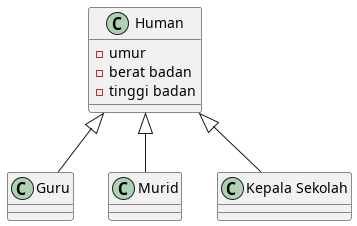
\includegraphics[width=8cm]{inheritance example.png}
              \caption{Contoh dari \textit{inheritance}}
          \end{figure}

    \item \textit{Polymorphism}

          \textit{Child class} adalah sebuah \textit{class} yang akan menuruni semua atribut dan fitur dari \textit{parent class}, tapi apabila dari satu \textit{parent class} memiliki 2 \textit{child class} yang memiliki fitur yang sama tapi cara melakukannya yang berbeda? contoh pisang goreng adalah sebuah makanan, tapi tidak semua makanan adalah pisang goreng, ada perubahan dari cara memasak dan cara penyajian ditiap - tiap makanan, disini konsep \textit{polymorphism} dapat dipakai. Secara definisi \textit{polymorphism} adalah kelakuan dimana \textit{child class} bisa melakukan suatu \textit{task} atau fitur yang sama seperti \textit{parent class} dengan cara yang berbeda\autocite{education-erin-oop-2020}.
\end{enumerate}


% \newpage
\subsubbab{\textit{Functional Programming}}
\textit{Functional Programming} adalah sebuah konsep, paradigma atau sebuah macam \textit{software development} yang menekankan titik beratnya pada penggunaan \textit{functions}, \textit{Functional Programming} sendiri bukan merupakan sebuah alat yang dapat digunakan tetapi merupakan sesuatu pegangan untuk \textit{developers} sebagai sebuah cara menulis kode\autocite{atencio2016functional}.


Tujuan dari \textit{Functional Programming} adalah membuat sebuah \textit{function} yang lebih kecil yang memiliki sifat dapat digunakkan kembali, lebih dapat diandalkan dan mudah dimengerti, lalu \textit{functions} tersebut maka akan dapat membuat sebuah program yang lebih dapat dimengerti \autocite{atencio2016functional}. \textit{Function} yang dibuat mengikuti \textit{Functional Programming} biasa dibuat dengan melakukan parameterisasi pada \textit{function} supaya dalam menggunakannya dengan menggunakkan parameter kode tersebut dapat digunakkan kembali untuk melakukan hal yang lain. \textit{Functional Programming} memiliki empat konsep dasar, yaitu \textit{Declarative programming}, \textit{Pure functions}, \textit{Referential transparency}, dan \textit{Immutability}\autocite{atencio2016functional}.


\begin{itemize}
    \item \textit{Declarative programming} adalah sebuah pendekatan \textit{programming} dimana sebuah kode untuk melakukan sesuatu akan ditulis menggunakan \textit{expressions} yang mendeskripsikan logika dari suatu program. Berbeda dengan Imperatif atau \textit{Procedural Programming} dimana akan ditulis secara detail bagaimana untuk melakukan sesuatu untuk mencapai hasil yang diinginkan\autocite{atencio2016functional}.
    \item \textit{Pure functions} adalah \textit{function} yang memiliki dua sifat, yaitu pertama, sebuah pure function hanya dan hanya bergantung pada input yang diberikan dan tidak dengan \textit{state} yang tersembunyi dan/atau external (diluar function tersebut) dan kedua, tidak merubah apapun yang diluar dari \textit{function} tersebut seperti obyek global atau parameter yang di \textit{pass} ke \textit{function} tersebut \autocite{atencio2016functional}.
    \item \textit{Referential transparency} adalah ketika sebuah \textit{function} menghasilkan hasil yang sama juga diberikan input yang sama \autocite{atencio2016functional}.
    \item \textit{Immutability} adalah dimana dalam \textit{Functional Programming} untuk melestarikan sebuah data supaya \textit{Immutable} tidak bisa diganti setelah di deklarasi. Dalam konsep ini yang perlu diperhatikan adalah object seperti \textit{array} yang dapat berubah konten atau valuenya dalam sebuah function \autocite{atencio2016functional}.
\end{itemize}

\subsubbab{\textit{Architectural Pattern}}
\textit{Architectural Pattern} merupakan seperangkat prinsip dan pola kasar yang menyediakan kerangka kerja abstrak dari sebuah sistem. \textit{Architectural Pattern} menggambarkan struktural fundamental dari suatu organisasi atau skema untuk sebuah sistem yang kompleks. \textit{Architectural Pattern} dapat digunakan sebagai solusi umum yang dapat digunakan kembali \textit{(reusable)} untuk memecahkan permasalahan yang biasa terjadi dalam sebuah \textit{software architecture} di dalam konteks tertentu\autocite{architectural-pattern}. Dalam artian, \textit{Architectural Pattern} mirip dengan \textit{Design Pattern}, tetapi memiliki cakupan yang lebih luas\autocite{archi-pattern}.
\begin{itemize}
    \item \textit{Object-Oriented Architecture (OOA)}\\
          \textit{Object-Oriented Architecture} dapat digunakan jika ingin mengenkapsulasi logika dan data bersama-sama dalam komponen yang dapat digunakan kembali. \textit{Business Logic} yang kompleks yang membutuhkan abstraksi dan \textit{dynamic behaviour} dapat secara efektif menggunakan arsitektur jenis ini juga\autocite{architectural-pattern}.
    \item \textit{Layered/Tiered Architecture}\\
          \textit{Layered/Tiered Architecture} merupakan salah satu jenis \textit{architectural pattern} yang sangat sering digunakan\autocite{architectural-pattern}. Arsitektur jenis ini dapat digunakan untuk menyusun program yang dapat didekomposisikan menjadi beberapa kelompok \textit{subtasks}, yang masing-masing berada pada tingkat abstraksi tertentu. Setiap \textit{layer} menyediakan layanan \textit{(services)} ke \textit{layer} berikutnya yang lebih tinggi. Terdapat empat \textit{layer} utama di dalam arsitektur jenis ini, yakni \textbf{\textit{Presentation Layer}}, \textbf{\textit{Application Layer}}, \textbf{\textit{Business Logic Layer}} dan \textbf{\textit{Data Access Layer}}. Arsitektur jenis ini biasanya digunakan pada aplikasi desktop dan \textit{web e-commerce} pada umumnya\autocite{archi-pattern}.
    \item \textit{Event-Driven Architecture (EDA)}\\
          \textit{Event-Driven Architecture (EDA)} biasanya didasarkan pada \textit{communication model} yang digerakkan oleh pesan asinkron untuk menyebarkan informasi ke seluruh organisasi/perusahaan. \textit{EDA} mendukung \textit{allignment} yang lebih alami dengan model operasional organisasi dengan menggambarkan \textit{business activity} nya sebagai suatu rangkaian \textit{event}/peristiwa\autocite{architectural-pattern}.
    \item \textit{Model-View-Controller Architecture (MVC)}\\
          \textit{Model-View-Controller Architecture} atau biasa juga disebut sebagai \textbf{MVC}, merupakan sebuah jenis \textit{architectural pattern} yang membagi sistem aplikasinya menjadi tiga bagian, yakni \textbf{\textit{Model}}, \textbf{\textit{View}} dan \textbf{\textit{Controller}}. \textbf{\textit{Model}} merupakan fungsi inti dari aplikasi dan menyimpan data, \textbf{\textit{View}} merupakan sebuah \textit{user interface} (\textbf{UI}) yang dapat dilihat atau berinteraksi dengan pengguna secara langsung dan \textbf{\textit{Controller}} sebagai penghubung antara \textit{model} dengan \textit{view} serta yang mengatur \textit{input} dari pengguna. Arsitektur jenis ini paling sering digunakan untuk membuat sebuah aplikasi berbasis web\autocite{archi-pattern}.
\end{itemize}

\subsubbab{\textit{Design Pattern}}
\textit{Design Pattern} secara definisi adalah sesuatu cara komunikasi tiap obyek dan \textit{class} yang dikostumisasi untuk memecahkan masalah desain general di dalam konteks tertentu, \textit{design pattern} membantu untuk membuat \textit{object oriented design} yang dapat digunakan secara berulang, dengan cara memberi nama, mengabstraksi, dna mengidentifikasi kunci aspek dari struktur desain tertentu\autocite{design-pattern-2588942}.
\begin{itemize}
    \item \textit{Facade}\\
          \textit{Facade} adalah sesuatu \textit{class} yang memberikan \textit{interface} yang simpel ke sub-sistem yang kompleks, \textit{design pattern} ini dapat digunakan ketika butuh mengintegrasikan sesuatu \textit{library} dengan fitur yang sangat banyak tapi hanya butuh menggunakan beberapa fiturnya saja\autocite{refactoring-guru}. \textit{Singleton} juga memberikan global \textit{access point} ke instansi \textit{class} tersebut, jadi semua \textit{class} dan \textit{object} dapat membaca \textit{value} yang sama dan merubah \textit{value} tersebut secara keseluruhan\autocite{refactoring-guru}.
    \item \textit{Singleton}\\
          \textit{Singleton} digunakan untuk menjamin bahwa suatu \textit{class} hanya memiliki satu \textit{instance}, \textit{design pattern} ini berguna saat ingin mengontrol sebuah \textit{shared resources} seperti \textit{database}\autocite{refactoring-guru}.
    \item \textit{Builder}\\
          \textit{Design pattern} ini dibuat untuk memecahkan masalah ketika ada sebuah \textit{class} yang saat dibuat menjadi sebuah \textit{object} tidak semua atributnya diisi, tanpa harus membuat \textit{contructor} atau \textit{child class} banyak. \textit{Builder} mengekstrasi \textit{building steps} saat membuat suatu \textit{object} dari sebuah \textit{class} dan memindahkannya ke \textit{class} terpisah\autocite{refactoring-guru}.
    \item \textit{Template Method}\\
          \textit{Template method} digunakan untuk mengurangi redudansi ketika ada beberapa fitur dengan langkah penyelesaian sama tapi dengan cara yang berbeda, \textit{template method} dibuat dengan cara memisahkan logika suatu fitur menjadi beberapa langkah dan saat ingin menambahkan fitur baru, bisa langsung membuat \textit{child class} dari \textit{template method} tersebut dan meng-\textit{override} step yang ingin diganti logikanya\autocite{refactoring-guru}.
\end{itemize}

\subsubbab{\textit{Software Testing}}

Secara general manusia pasti akan melakukan kesalahan, apa lagi di dalam \textit{software development} hal ini sangat kelihatan saat dengan pasti adanya \textit{bug} di dalam \textit{software} yang dikerjakan, ini adalah salah satu alasan kenapa \textit{software testing} itu dibutuhkan, untuk menemukan masalah dan memperbaikinya. Alasan satu lagi \textit{software testing} dilakukan adalah untuk membuat keputusan, apakah \textit{software} yang sedang dibuat ini sudah mempunyai kualitas yang dapat diterima \autocite{jorgensen2018software}.

Secara definisi dasar, \textit{software testing} adalah suatu metode untuk mengecek apakah sebuah produk atau \textit{software} sudah sama dengan kebutuhan - kebutuhan dan memastikan \textit{software} tersebut tidak memiliki kecacatan\autocite{guru99-software-testing}.

\textit{Software testing} bisa digeneralisasikan menjadi 2 tipe, yaitu:
\begin{itemize}
    \item \textit{Blackbox testing}

        \textit{Blackbox testing} atau sering disebut \textit{specification-based testing}, adalah testing yang dilakukan berdasarkan dengan spesifikasi \textit{software} tersebut. Metode testing ini disebut \textit{blackbox testing} karena sebuah sistem atau program itu akan dianggap seperti kotak hitam yang tidak bisa dilihat isinya, tapi diketahui apa saja yang bisa dilakukan oleh kotak hitam tersebut\autocite{jorgensen2018software}.

        Kelebihan dari metode \textit{testing} ini adalah, \textit{unit test} yang dibuat itu berdiri sendiri dari bagaimana implementasi yang ada di dalam \textit{software} tersebut, jadi jika ada perubahan implementasi \textit{test case} yang sebelumnya dibuat akan tetap bisa dipakai dan \textit{testcase} untuk \textit{blackbox testing} dapat dibuat saat masa \textit{development} sedang berjalan, jadi bisa mengurangi masa pengerjaan \textit{project}\autocite{jorgensen2018software}.


    \item \textit{Whitebox testing}

        \textit{Whitebox testing} adalah metode \textit{testing} yang dimana semua struktur internal, desain, dan implementasi dites untuk memperbaiki desain, kegunaan, dan keamanan. Terminologi \textit{whitebox} ini menganggap \textit{software} itu seperti box yang transparan, dimana semua isinya (implementasi dari sebuah fungsi dan pilihan desain yang diambil) akan kelihatan dalam fase pengetesan\autocite{guru99-whitebox-testing}.

        Salah satu tipe \textit{whitebox testing} adalah \textit{unit testing}. \textit{Unit testing} adalah \textit{test case} yang biasanya ditulis oleh \textit{developer} untuk melakukan pengetesan disetiap blok kode yang sedang dikembangkan\autocite{guru99-whitebox-testing}. Ada dua teknik yang bisa diterapkan saat melakukan \textit{whitebox testing}, yaitu:
        \begin{itemize}
            \item \textit{Statement Coverage}

            teknik ini membutuhkan semua \textit{statement} yang ada di dalam \textit{code base} sudah tertutupi oleh \textit{test case} dari \textit{whitebox testing}.
 
            \item \textit{Branch Coverage}

            teknik ini membutuhkan semua \textit{branch} atau \textit{path} yang ada di dalam \textit{code base} sudah tertutupi oleh \textit{test case} dari \textit{whitebox testing}.
        \end{itemize}
\end{itemize}

\subsubbab{Sistem Rekomendasi}
Sistem rekomendasi adalah sistem penyaringan informasi yang menyarankan sebuah produk kepada pengguna berdasarkan preferensi atau perilaku masa lalu. Sistem ini banyak digunakan di pasar \textit{online} untuk meningkatkan pengalaman, keterlibatan pengguna, dan mendorong penjualan. Dengan memberikan rekomendasi yang dipersonalisasi terhadap preferensi, pengguna dapat menemukan sebuah barang yang mungkin tidak bisa ditemukan sendiri dan meningkatkan kepuasan pengguna terhadap pasar \textit{online} yang sedang digunakan \autocite{adiwardana2019}.

Kenapa sistem rekomendasi ini dibutuhkan telah dibuktikan oleh sebuah artikel yang diterbitkan pada tahun 2019 oleh Tian \textit{et al}. yang berjudul "\textit{Exploring the effects of personalized recommendation on users' satisfaction and loyalty in e-commerce}" yang menemukan bahwa pengguna \textit{platform e-commerce}  akan menghabiskan waktu 50\% lebih banyak di \textit{platform} tersebut ketika pengguna diberikan sebuah rekomendasi produk yang dipersonalisasi\autocite{tian2019exploring}. Sistem rekomendasi juga menguntungkan untuk mengurangi terjadinya \textit{information overload} yang akan dialami oleh pengguna, dengan cara hanya menampilkan produk yang ingin dilihat atau yang sesuai dengan preferensi - preferensi pengguna tersebut\autocite{karimi2018news}.

Sistem rekomendasi yang akan dipakai di dalam proyek ini akan berdasarkan pada teori \textit{Knowledge Graph}. \textit{Knowledge Graph} adalah sebuah \textit{graph} heterogen, dimana \textit{nodes} akan merepresentasikan sebuah hubungan antara entitas\autocite{guo2020survey}. Dengan menggunakan teori ini, semua produk dan atribut - atributnya dapat dibuat menjadi sebuah \textit{graph} untuk mempermudah memahami hubungan antara tiap produk, selain itu informasi pengguna dan preferensi mereka-pun bisa diintegrasikan ke-\textit{graph} tersebut untuk membantu prediksi rekomendasi menjadi seakurat mungkin.

\begin{figure}[h]
    \centering
    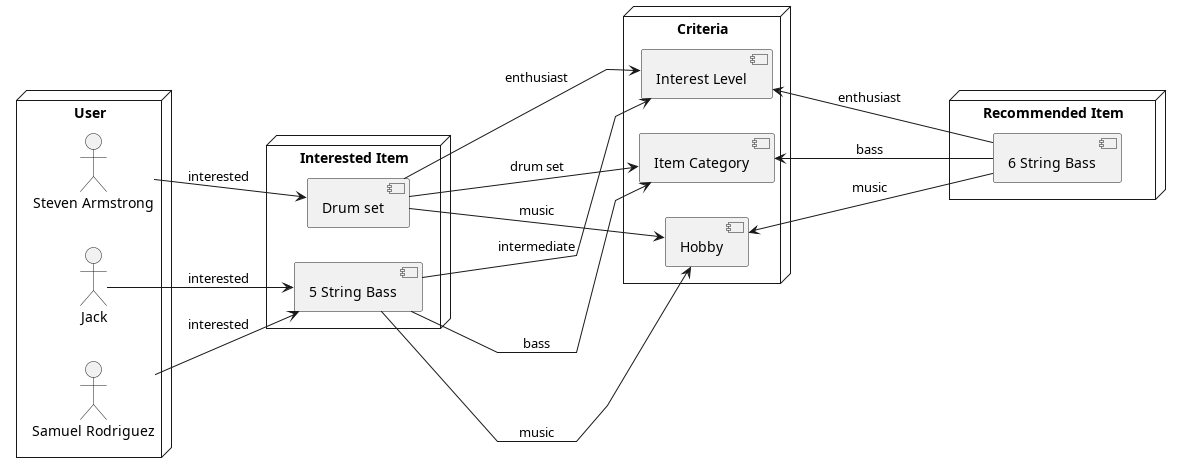
\includegraphics[width=8cm]{recommendation system architecture.png}
    \caption{Contoh simpel dari sistem rekomendasi dengan basis \textit{Knowledge Graph}}
\end{figure}

\subsubbab{\textit{Caching}}
Secara definisi \textit{caching} adalah sebuah \textit{data storage layer} yang bersifat sementara dan digunakan untuk mempercepat permintaan data dibanding mengakses lokasi penyimpanan utama data tersebut. Fungsi utama \textit{cache} adalah menurunkan proses permintaan data ke lokasi penyimpanan utama yang lambat dengan cara menaruh data tersebut ke \textit{storage layer} yang lebih cepat seperti RAM\autocite{AWS-caching}. Berikut adalah kelebihan dari sistem \textit{caching}:

\begin{itemize}
    \item \textit{Cache} membuat semuanya berjalan lebih cepat. Manfaat utama dari cache adalah menurunkan \textit{response time} yang dibutuhkan untuk memproses sebuah \textit{request}. Seperti contoh, dengan menyimpan salinan lokan file dari sebuah \textit{website} saat pertama kali dikunjungi, pada kunjungan berikutnya browser tidak perlu membuang waktu dan sumber daya untuk mengunduh informasi tersebut karena sudah disimpan di penyimpanan lokal\autocite{businessinsider_cache}.

    \item Menghilangi \textit{Database Hotspot}. Dibanyak aplikasi kemungkinan hanya sebagian kecil data yang akan diakses lebih sering dibandingkan dengan data lainnya, seperti \textit{profile} selebriti yang terkenal atau produk yang diminati banyak orang. Hal ini dapat menyebabkan \textit{hot spots} di \textit{database} yang digunakan dan mungkin memerlukan penyediaan \textit{resource database} yang berlebihan berdasarkan \textit{throughput} atau jumlah data yang dapat ditangani\autocite{AWS-caching}. \textit{Cache} mengatasi hal ini dengan memunkinkan \textit{software} untuk mengakses memori lokalnya seperti RAM dibandingkan membuat \textit{request} untuk meng-\textit{query} data dari \textit{database}, yang dapat menjadi operasi yang mahal.

    \item \textit{Cache} juga bisa mengurangi beban di \textit{backend}, dengan cara mengalihkan sebagian besar beban operasi \textit{query} ke memori lokal dari \textit{database backend}, hal ini akan mencegah terjadinya performa yang menurun atau \textit{crashing} ketika ada lonjakan \textit{traffic}.
\end{itemize}



\subsubbab{\textit{Asynchronous Processing}}
\textit{Asynchronous Processing} adalah kebalikan dari \textit{synchronous processing} yang akan mengeksekusi setiap proses secara linear sesuai dengan berjalannya waktu. Sebagai contoh, diberikan dua pemanggilan ke '\textit{request.get}' dalam \textit{synchronous processing} pemanggilan kedua tidak akan dijalankan sebelum pemanggilan pertama sudah selesai. Sedangkan dengan menggunakan model \textit{asynchronous processing} dua pemanggilan tersebut bisa dilakukan secara bersamaan\autocite{Williams_Benfield_Warner_Zadka_Mitchell_Samuel_Tardy_2019}.

\subsubbab{\textit{Agile Scrum}}
\textit{Agile} adalah kumpulan metodologi yang bisa membantu tim yang men-\textit{develop} suatu proyek untuk berfikir dan bekerja lebih efisien dan membantu untuk mengambil keputusan yang lebih baik\autocite{Stellman_Greene_2016}. Salah satu dari metodologi tersebut adalah \textit{scrum}, \textit{scrum} adalah \textit{project management framework} yang membantu tim untuk menyusun dan mengelola \textit{task - task} yang ada dengan serangkaian nilai, prinsi, dan praktik\autocite{atlassian-agile-scrum}.

\begin{figure}[h]
    \centering
    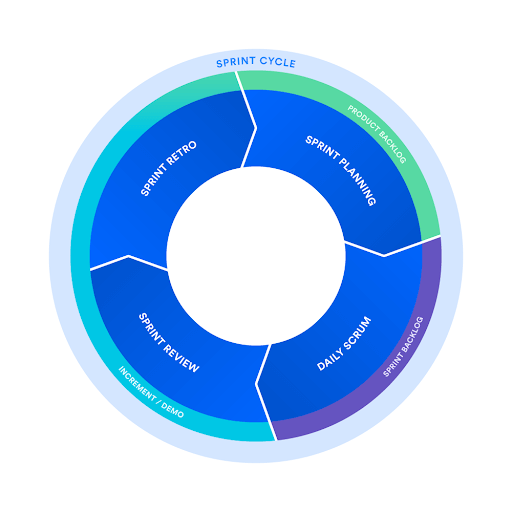
\includegraphics[width=6cm]{images/sprint_cycle-c.png}
    \caption{Contoh dari struktur \textit{scrum}\autocite{atlassian-agile-scrum}}
    \label{fig:strukturagile}
\end{figure}

Walaupun \textit{scrum} itu memiliki struktur, namum implementasi dari \textit{scrum} sendiri dapat disesuaikan dengan kebutuhan organisasi atau tim yang sedang menggunakan \textit{scrum}, secara umum \textit{scrum framework} itu memiliki enam kunci kegiatan yang mungkin diikuti oleh tim \textit{scrum}:
\begin{enumerate}
    \item \textit{Backlog grooming}, kegiatan ini adalah tanggung jawab dari \textit{product owner} yang bertujuan membantu tim \textit{scrum} untuk terus menyempurnakan, memprioritaskan, dan memperjelas \textit{item backlog} dibantu dari masukan \textit{users} dan tim \textit{developement}.

    \item \textit{Sprint planning} adalah kegiatan untuk mendefinisikan '\textit{scope}' atau batasan - batasan yang akan dikerjakan oleh tim \textit{development} di \textit{sprint} yang akan datang dan memastikan \textit{user stories} yang akan dikerjakan itu bisa dikerjakan dan diimplementasikan selama \textit{sprint}.

    \item \textit{Sprint} adalah waktu (biasanya dua minggu) yang dipakai untuk mengerjakan semua \textit{user stories} yang sudah didefinisikan pada fase \textit{sprint planning}. 

    \item \textit{Daily Scrum} adalah sebuah \textit{meeting} yang singkat setiap hari (biasanya pagi hari) yang diadakan untuk tim \textit{development} melakukan diskusi jika ada halangan dalam mengerjakan \textit{task} dan memberikan \textit{update} tentang \textit{task}.

    \item \textit{Sprint Review}, adalah \textit{meeting} yang dilaksanakan setelah sebuah \textit{sprint} selesai, dimana semua tim yang berpartisipasi untuk meminta feedback terhadap semua \textit{user stories} yang berhasil dikerjakan di \textit{sprint} ini.

    \item \textit{Sprint Retro}, adalah \textit{meeting} dimana semua tim yang berpartisipasi berkumpul untuk mendiskusikan apa saja yang bekerja dengan lancar dan apa saja yang tidak bekerja sama sekali atau mengalami kendala. Idenya adalah \textit{meeting} ini akan membuat tim \textit{scrum} tempat untuk berdiskusi apa saja yang perlu diperbaiki di \textit{sprint} kedepannya.
\end{enumerate}

\subsubbab{\textit{Hobby}}
\textit{Hobby} atau hobi secara singkat adalah sebuah kegiatan yang dilakukan oleh seorang dalam waktu luang untuk mendapatkan kesenangan \autocite{Dict_hobi}. Seseorang dapat mengadopsi dan memulai hobi dapat karena untuk mengisi waktu luangnya dan mendapatkan kesenangan dan rasa kepenuhan dari itu \autocite{linkedin_hobi}.

\subsubbab{\textit{Interest Level}}
\textit{Interest Level} adalah suatu pengelompokkan yang dibuat untuk mempermudah memisahkan antara pemilik hobi yang digolongkan dari tingkat kemahiran mereka dalam sebuah hobi tertentu. Ada tiga level yang kami buat, yaitu \textit{BEGINNER}, \textit{INTERMEDIATE}, dan \textit{ENTHUSIAST}. Klasifikasi tersebut akan diberikan kepada barang oleh penjual dan pengguna yang sudah membeli barang bersangkutan. Klasifikasi atau pengelompokan tersebut pada barang bertujuan untuk memisahkan barang yang tepat bagi tingkat kemahiran tertentu dengan yang lain. Sehingga dengan tujuan agar barang yang tergolong \textit{BEGINNER} merupakan barang yang cocok untuk pemula, seseorang yang memulai suatu hobi.

\subsubbab{\textit{E-commerce}}
\textit{E-commerce} merupakan aktivitas jual beli barang atau jasa dan juga pengiriman dana yang dilakukan melewati sebuah jasa \textit{online} atau melalui internet. Cara kerja \textit{e-commerce} adalah dengan pelanggan mengakses sebuah aplikasi toko online dan membuat pesanan dan membayar untuk pesanan tersebut yang prosesnya akan diatasi atau diproses oleh  aplikasi tersebut. \autocite{techtarget_e-commerce}.

\subsubbab{\textit{Online Marketplace}}
\textit{Online Marketplace} adalah sebuah tipe dari \textit{e-commerce} yang dimana  produk atau jasa yang ada di aplikasi berasal dari pihak ketiga yang dapat mendaftarkan diri untuk menjual barang atau jasa di tempat aplikasi \textit{online marketplace}. \autocite{pediaa_marketplace}

\subsubbab{\textit{Marketing}}
\textit{Marketing} adalah sebuah aktivitas yang dilakukan oleh sebuah pihak untuk membuat sebuah dorongan untuk menarik kegiatan membeli atau menjual barang atau jasa \autocite{Twin_2023}. Aktivitas untuk melakukan dorongan tersebut adalah aktivitas yang dapat mengidentifikasikan dan mengantisipasikan kebutuhan pengguna dan mencoba untuk memenuhi kebutuhan tersebut \autocite{openStax}.

\subsubbab{\textit{Responsive Web Design} dan \textit{Mobile-First Design}}
\textit{Responsive Web Design} adalah presentasi dan cara menampilkan isi konten dari sebuah website dengan format yang paling cocok dan relevan dengan perangkat yang mengakses \autocite{Frain_2022}. \textit{Mobile-First Design} adalah konsep yang mengajukan bahwa dalam mendesain dan implementasi aplikasi dimulai dari resolusi layar atau perangkat yang kecil terlebih dahulu dan menambahkan styling dan implementasi untuk resolusi layar yang lebih besar \autocite{Ward_2017}.

\subsubbab{\textit{Five Measurable Human Factor}}
\textit{Five Measurable human factor} adalah sebuah tes yang dapat dilakukan terhadap sebuah aplikasi dengan cara mencatat 5 kriteria bagaimana seorang manusia berinteraksi dengan sistem informasi aplikasi dan menafsirkan sebuah penilaian dari seberapa baik atau lancarnya seseorang dapat menggunakannya sesuai dengan 5 kriteria tersebut \autocite{Shneiderman_Plaisant_Cohen_Jacobs_Elmqvist_2018_5_factors}. Kelima faktor tersebut adalah:
\begin{enumerate}
    \item \textit{Time for users to learn specific functions}\\
    Waktu yang diperlukan oleh pengguna untuk mempelajari cara menggunakan dan menavigasikan sebuah aplikasi.
    \item \textit{Speed of task performance}\\
    Seberapa cepat pengguna melaksanakan suatu fungsi yang ada pada aplikasi hingga selesai
    \item \textit{Rate of errors by users}\\
    Berapa banyaknya \textit{error} yang ditemui, dihadapi oleh pengguna dalam menggunakan aplikasi dan menjalankan sebuah aksi untuk mencapai hasil dari suatu fungsi.
    \item \textit{User retention of commands over time}\\
    Berapa lama pengguna dapat mengingat informasi mengenai aplikasi setelah rentan waktu seperti beberapa hari atau lebih.
    \item \textit{Subjective user satisfaction}\\
    Pengukuran seberapa puas pengguna dari aspek manapun aplikasi.
\end{enumerate}

\subsubbab{\textit{The Eight Golden Rules of Interface Design}}
\textit{The Eight Golden Rules of Interface Design} adalah sebuah lis yang memiliki poin-poin yang dapat menjadi panduan bagi desainer dan murid atas apa yang dapat dites dari sebuah sistem interaktif \autocite{Shneiderman_Plaisant_Cohen_Jacobs_Elmqvist_2018_eight_golden_rules}. Berikut adalah kedelapan \textit{Golden Rules} yang ditulis:
\begin{enumerate}
    \item \textit{Strive for consistency}\\
    Dalam suatu konsistensi adalah hal yang baik di dalam segala hal pada suatu sistem interaksi. Seperti urutan aksi untuk mencapai suatu diusahakan konsisten dan mirip dengan aksi untuk mencapai suatu yang mirip. Contoh lainnya adalah penggunaan kata atau istilah seharusnya konsisten di keseluruhan, sama halnya dengan penggunaan warna, tata letak, bahkan font kata. Dan jika harus ada yang tidak konsisten karena diperlukan, diusahakan sesedikit mungkin.
    \item \textit{Seek universal usability}\\
    Penambahan fitur untuk segala macam pengguna, seperti fitur untuk membantu pemula dalam teknologi seperti penjelasan atau fitur untuk yang ahli supaya mendapatkan \textit{shortcuts} untuk mempercepat penggunaan akan mendorong rasa kualitas.
    \item \textit{Offer informative feedback}\\
    Tiap kali pengguna melakukan suatu hal, ada baiknya dan seharusnya ada respons yang sesuai dari aplikasi.
    \item \textit{Design dialogs to yield closure}\\
    Dalam suatu proses aksi pada aplikasi, informasi status proses aksi seharusnya dikomunikasikan jika sudah selesai atau hasil akhir dari aksi yang dilakukan, seperti jika pengguna ingin memasukan barang ke sebuah \textit{wishlist}, dikomunikasikan jika berhasil atau gagal.
    \item \textit{Prevent errors}\\
    Poin ini berfokus untuk menjaga pengguna dari melakukan sesuatu hal yang dapat menimbulkan sebuah \textit{error}/kerusakan yang serius, dan jika terjadi \textit{error} pada tinggi tingkat manapun harus ada panduan dari aplikasi yang mudah dimengerti, konstruktif dan spesifik untuk membetulkannya.
    \item \textit{Permit easy reversal of actions}\\
    Pada aplikasi sebanyak mungkin mendukung pembalikan atau membatalkan aksi. Seperti jika pengguna menambah barang yang salah ke \textit{cart}, seharusnya untuk menghapus barang tersebut mudah. Ini supaya pengguna tidak merasa takut untuk melakukan eksplorasi dan mengenal aplikasi.
    \item \textit{Keep users in control}\\
    \textit{Rule} ini mendorong agar sebuah aplikasi memberi rasa bahwa pengguna menguasai sebuah aplikasi. Contoh dari rasa ini adalah pengguna dalam menggunakan aplikasi tiap aksi yang dilakukan pengguna ada respons yang cocok, pengguna mengenal dan mengetahui aksi dan karakteristik aplikasi, pengguna mudah untuk melakukan hal apapun, mudah mendapatkan informasi dan juga pengguna dapat mencapai tujuan dan membuat hasil yang mereka inginkan.
    \item \textit{Reduce short-term memory load}\\
    Pentingnya bagi aplikasi tidak meminta pengguna untuk mengingat suatu data dari halaman satu di halaman yang lain. Oleh karena itu data-data yang diperlukan yang dapat diakses oleh aplikasi seperti data pengguna yang sudah tersimpan tidak perlu pengguna yang menulis/mengisi-nya lagi kembali. Dan juga untuk mengisi formulir sebaiknya hanya 1 halaman saja dan tidak terpisah-pisah.
\end{enumerate}

\subsubbab{\textit{Document Object Model}}
\textit{Document Object Model} (\textbf{DOM}) adalah sebuah antarmuka untuk dokumen web yang memungkinkan akses dan manipulasi terhadap dokumen web tersebut. Dengan bahasa pemrograman \textit{scripting} seperti \textit{JavaScript} dapat mengakses melalui antarmuka dari DOM dan melakukan perubahan atau penambahan elemen atau konten pada halaman web \autocite{DOM_teori}.



\subsubbab{Internet}
Internet merupakan sebuah bentuk dari infrastruktur jaringan komunikasi global yang menghubungkan miliaran komputer (ataupun perangkat lainnya) satu sama lain yang tersebar di seluruh dunia\autocite{javatpoint-internet}. Kata "Internet" sendiri berasal dari bahasa latin, yakni dari kata "\textit{inter}" dan "\textit{net}". Kata "\textit{inter}" memiliki arti sebagai "antara" dan kata "\textit{net}" yang berarti "jaringan". Kata "\textit{net}" ini jugalah yang merupakan singkatan dari kata \textit{network}\autocite{arti-kata-internet}. Internet dibangun/di-\textit{setup} dengan menggunakan bantuan transmisi data dari kabel-kabel \textit{fiber optic} atau kabel tembaga dan berbagai macam media jaringan lainnya\autocite{gfg-internet}. Ada beberapa istilah penting yang sangat berhubungan dengan jaringan internet, seperti:
\begin{itemize}
    \item \textit{Client}\\
    \textit{Client} merupakan sebuah istilah yang digunakan untuk mendefinisikan perangkat-perangkat pengguna (\textit{end-user devices}) yang tersambung langsung ke internet dan meminta/me-\textit{request} layanan kepada server. Contoh, sebuah laptop atau \textit{smartphone} yang tersambung ke wifi dan meminta \textit{request} kepada server untuk mengunduh sebuah aplikasi\autocite{arti-client-server}.
    \item \textit{Server}\\
    \textit{Server} merupakan sebuah istilah yang digunakan untuk mendefinisikan perangkat komputer besar yang bertugas untuk memberikan layanan kepada perangkat lain yang tersambung dengan jaringan internet. Contoh, sebuah server yang memberikan layanan kepada \textit{end-user devices} untuk mengunduh suatu aplikasi\autocite{arti-client-server}.
    \item \textit{Internet Service Provider} (ISP)\\
    \textit{Internet Service Provider} atau yang biasa disebut sebagai ISP, merupakan sebuah organisasi yang menyediakan layanan untuk mengakses, menggunakan, mengelola atau ikut berpartisipasi di dalam jaringan internet. ISP dapat berbentuk sebagai organisasi komersial, organisasi milik komunitas, \textit{non-profit} atau bahkan milik pribadi\autocite{what-is-isp}.
    \item \textit{IP Address}\\
    \textit{IP Address} merupakan sebuah alamat unik yang mengidentifikasi sebuah perangkat di dalam jaringan internet, layaknya sebuah alamat rumah yang mengidentifikasi lokasi/tempat rumah tersebut berada. Dalam kata lain, \textit{IP Address} adalah sebuah alat pengidentifikasi yang memungkinkan pengiriman informasi antarperangkat dan berisikan informasi lokasi yang memungkinkan sebuah perangkat dapat diakses untuk komunikasi di dalam jaringan internet\autocite{what-is-ip-address}. \textit{IP Address} terdiri dari sederetan angka yang dipisahkan oleh tanda titik (.). Deretan angka pada \textit{IP Address} itu adalah unik, sehingga bentuk deretannya dapat berbeda-beda dari satu perangkat dengan perangkat lainnya\autocite{javatpoint-internet}. Contoh bentuk dari \textit{IP Address}: 192.168.10.69
    \item \textit{Domain Name System} (DNS)\\
    \textit{Domain Name System} atau biasa disebut sebagai DNS, merupakan sebuah alat yang bertugas untuk menerjemahkan \textit{IP Address} menjadi suatu nama domain (\textit{domain name})\autocite{what-is-dns}. Sedangkan (\textit{Domain name}) atau nama domain itu sendiri adalah sebuah rangkaian teks yang didapat dari pemetaan deretan angka pada \textit{IP Address} yang digunakan untuk mengakses sebuah situs web (\textit{website}). Contoh beberapa nama domain antara lain, 'google.com', 'twitter.com' dan 'binusmaya.binus.ac.id'\autocite{what-is-domain-name}. Pada dasarnya, DNS itu bagaikan sebuah buku telepon untuk internet. Pengguna dapat mengakses segala macam informasi secara \textit{online} melalui \textit{domain name} seperti 'yahoo.com' atau 'youtube.com', yang kemudian diketik melalui sebuah \textit{web browsers} seperti Google Chrome atau Firefox. Lalu \textit{web browser} tersebut berinteraksi melalui \textit{IP Address} yang kemudian \textit{domain name} yang di \textit{request} sebelumnya dapat diterjemahkan oleh DNS menjadi \textit{IP Address} yang sesuai sehingga \textit{web browser} dapat memuat informasi yang diinginkan oleh penggunanya\autocite{what-is-dns}.
    \item \textit{Web Browser, Web Page, Website} dan \textit{Web Server}
    \begin{itemize}
        \item \textit{Web Browser}\\
        \textit{Web Browser} merupakan sebuah aplikasi perangkat lunak yang digunakan untuk menelusuri, mengakses dan memuat berbagai macam \textit{web page} yang tersedia di internet\autocite{web-browsers}.
        \item \textit{Web Page}\\
        \textit{Web Page} merupakan sebuah dokumen/halaman yang dapat ditampilkan pada \textit{web browser}. \textit{Web Page} ini biasa juga disebut sebagai "\textit{pages}"\autocite{webpage-website-webserver}.
        \item \textit{Website}\\
        \textit{Website} adalah sebuah koleksi dari \textit{web page} yang dikelompokkan dalam suatu kelompok bersamaan dan biasanya saling terhubung satu sama lain. \textit{Website} biasanya juga disebut sebagai "\textit{site}"\autocite{webpage-website-webserver}.
        \item \textit{Web Server}\\
        \textit{Web Server} merupakan sebuah aplikasi perangkat lunak yang dihosting pada komputer khusus yang berguna untuk memberikan/menampilkan \textit{website} ketika di-\textit{request} oleh \textit{web browser}\autocite{web-browsers}.
    \end{itemize}
    \item \textit{Internet Connection Protocols}\\
    Saat melintasi di dalam jaringan internet, data yang dikirim tersebut terlebih dahulu dipecah menjadi bagian-bagian yang lebih kecil yang dinamakan sebagai "\textit{packet}". Informasi IP terlampir pada tiap paket yang ada, dan informasi IP inilah yang membantu merutekan jalan agar pengiriman paket tersebut tiba di tempat tujuan yang tepat. Tempat tujuan dari paket-paket ini adalah alamat IP (\textit{IP Address}) dari masing-masing perangkat/domain yang terhubung dengan internet\autocite{what-is-internet-protocol}. Maka dari itu, agar pengiriman paket-paket ini berjalan dengan lancar, maka dibutuhkannya sebuah sistem protokol yang dapat membantu dan menjaga pengiriman paket-paket saat dikirimkan melewati internet.
    \textit{Internet Connection Protocols} (IP) merupakan sebuah protokol atau seperangkat aturan yang digunakan untuk \textit{routing}/perutean dan menangani pengiriman paket data agar dapat berjalan melintasi jaringan internet dan tiba di tempat tujuan yang tepat\autocite{what-is-internet-protocol}. Berikut adalah beberapa macam jenis \textit{Internet Protocols} yang sering digunakan:
    \begin{itemize}
        \item TCP/IP (\textit{Transmission Control Protocol/Internet Protocol})\\
        TCP/IP merupakan salah satu bentuk dari protokol transport, yang berarti protokol ini menentukan cara datanya dikirim dan diterima\autocite{what-is-internet-protocol}. Pada sistem protokol ini, protokol IP memastikan bahwa setiap perangkat yang terhubung dengan internet memiliki nomor seri yang khusus (\textit{IP Address}). Lalu, protokol TCP lah yang menentukan bagaimana data tersebut akan dipertukarkan melalui internet. TCP ini juga yang menentukan bagaimana data tersebut akan dipecah menjadi paket IP dan memastikan bahwa paket tersebut memiliki informasi mengenai sumber pengiriman data, tempat tujuan data yang dikirimkan, urutan pengiriman dari data tersebut serta memeriksa apakah data yang telah dikirim tiba di tempat tujuan yang benar\autocite{types-of-internet-protocols}.
        \item UDP/IP (\textit{User Datagram Protocol/Internet Protocol})\\
        Mirip seperti TCP/IP, UDP/IP juga merupakan sebuah protokol transport. Namun, UDP/IP ini bekerja lebih cepat dibandingkan TCP/IP, tetapi juga kurang dapat diandalkan. Karena, pada proses pengiriman paket datanya, protokol ini tidak memastikan bahwa paket yang terkirim tersebut berurutan/teratur sesuai dengan urutannya dan tidak membuat koneksi sebelum memulai atau menerima transmisi dalam proses pengiriman data\autocite{what-is-internet-protocol}.
        \item FTP (\textit{File Transfer Protocol})\\
        \textit{File Transfer Protocol} (FTP) adalah sebuah sistem protokol internet yang memungkinkan pengguna untuk mentransfer/memindahkan data berupa \textit{file} seperti dokumen, text, \textit{file} multimedia (gambar, video atau audio), sebuah \textit{program file}, dan lain sebagainya\autocite{javatpoint-internet}.
        \item HTTP (\textit{Hyper Text Transfer Protocol})\\
        Protokol jenis ini digunakan untuk mentransfer \textit{hypertext} (format text yang dapat berisi tautan ke text lain) melalui internet dan didefinisikan dengan "www" (\textit{World Wide Web}) untuk mentransfer informasi didalamnya. Protokol ini juga yang menentukan berbagai tindakan/\textit{action} yang harus dilakukan oleh \textit{web browser} sebagai \textit{response} atas panggilan yang dilakukan untuk mengakses \textit{web page} tertentu. HTTP inilah yang digunakan untuk berbagi berbagai macam \textit{file} multimedia di \textit{World Wide Web}\autocite{types-of-internet-protocols}.
    \end{itemize}
\end{itemize}

\subsubbab{\textit{API Call}}
\textit{Application Programming Interface} atau biasa juga disebut sebagai API, merupakan sekumpulan definisi dan protokol yang dapat digunakan untuk membangun dan mengintegrasikan aplikasi perangkat lunak\autocite{whats-api}. Adanya API memungkinkan para \textit{developer} untuk menghindari pekerjaan berulang yang berlebihan, alih-alih membangun dan membangun kembali fungsi aplikasi yang sudah ada, \textit{developer} dapat memasukkan yang sudah ada ke dalam aplikasi baru mereka dengan memformat permintaan sesuai kebutuhan API\autocite{whats-api-2}. \textit{API Calls} merupakan media yang digunakan untuk berinteraksi. Sebuah \textit{API Call} atau juga disebut sebagai \textit{API Request} adalah pesan yang dikirim ke server yang meminta API untuk menyediakan sebuah layanan atau informasi tertentu. \textit{API Calls} berpindah dari \textit{client} menuju ke \textit{API Endpoint} (tempat yang dituju oleh \textit{API Call}). \textit{API Endpoint} biasa berupa sebuah aplikasi web da server. Server tersebut menerima \textit{API Call}, lalu memprosesnya, mengeksekusinya dan mengirimkan respons yang dimana respons ini biasa disebut dengan istilah \textit{API Response}\autocite{whats-api-call}. Salah satu contoh nyatanya kegunaan dari API adalah misal, seseorang sedang mencari tiket hotel pada sebuah situs \textit{travel}. Situs tersebut kemudian mengirimkan \textit{API Call} ke beberapa perusahaan hotel dan menerima balik sebuah respons (\textit{API Response}) berupa informasi mengenai hotel-hotel tersebut, seperti lokasi hotel, jumlah kamar yang tersedia hingga harga penginapan untuk masing-masing jenis kamarnya.

\subsubbab{\textit{Flowchart}}
\textit{Flowchart} adalah sebuah visual representasi dari step-step dan keputusan yang harus dilakukan untuk melakukan sesuatu kegiatan, setiap step dilambangkan sebagai beberapa bentu dan dihubungkan panah terarah, karena itu \textit{flowchart} bisa menjadi alat yang ampuh untuk mengkomunikasikan sebuah proses seara efektif dan efisien\autocite{smartdraw-flowchart}.

Berikut ini adalah komponen-komponen dasar \textit{flowchart}
\begin{enumerate}
    \item Oval\\
    Bentuk ini melambangkan \textit{start} atau \textit{end}-nya dari sebuah proses.\\
    \begin{figure}[h]
        \centering
        \includegraphics*[width=2cm]{./diagram/flowchart/component/oval.png}
        \caption{Contoh bentuk oval dari komponen \textit{flowchart}}
    \end{figure}
    \item Persegi empat\\
    Bentuk ini menggambarkan sebuah proses.\\
    \begin{figure}[h]
        \centering
        \includegraphics*[width=2cm]{./diagram/flowchart/component/rectangle.png}
        \caption{Contoh bentuk segi empat dari komponen \textit{flowchart}}
    \end{figure}
    \newpage
    \item Jajar genjang\\
    Bentuk ini menggambar informasi yang memasuki atau dikeluarkan oleh sistem.\\
    \begin{figure}[h]
        \centering
        \includegraphics*[width=2cm]{./diagram/flowchart/component/jajar genjang.png}
        \caption{Contoh bentuk jajar genjang dari komponen \textit{flowchart}}
    \end{figure}
    \item Belah ketupat\\
        Bentuk ini melambangkan suatu pilihat atau keputusan yang harus diambil.\\
    \begin{figure}[h]
        \centering
        \includegraphics*[width=2cm]{./diagram/flowchart/component/diamond.png}
        \caption{Contoh bentuk belah ketupat dari komponen \textit{flowchart}}
    \end{figure}
    \item Panah\\
        Panah disini berlaku sebagai penanda arah berjalannya proses.
    \begin{figure}[h]
        \centering
        \includegraphics*[width=2cm,height=0.5cm]{./diagram/flowchart/component/arrow.png}
        \caption{Contoh panah dari komponen \textit{flowchart}}
    \end{figure}
\end{enumerate}

\newpage

\subsubbab{\textit{Unified Modeling Languages} (\textbf{UML})}
\textit{Unified Modeling Languages} atau biasa juga disebut sebagai UML merupakan sebuah bahasa pemodelan standar yang terdiri dari satu set diagram. Bahasa pemodelan yang terdiri dari diagram-diagram ini dikembangkan dengan tujuan untuk membantu para \textit{software developers} dan \textit{system developers} untuk membangun dan memvisualisasikan serta mendokumentasikan struktur sistem pada sebuah perangkat lunak (\textit{software}). Bahasa pemodelan ini juga dapat digunakan untuk memodelkan sebuah alur bisnis ataupun sebuah sistem yang bukan merupakan perangkat lunak (\textit{non-software system})\autocite{what-is-UML}.

Untuk sekarang, UML sudah berada di versi 2.5, yang dimana pada versi ini terdapat lima belas teknik diagram yang berbeda yang dapat digunakan untuk memodelkan suatu sistem. Diagram-diagram tersebut dibagi menjadi dua kelompok besar yakni, \textit{Structure Diagrams} yang digunakan untuk memodelkan struktur pada suatu sistem dan \textit{Behavioral Diagrams} yang digunakan untuk memodelkan alur kejadian/perilaku yang akan dijalankan pada sistem tersebut. \textit{Class Diagram} merupakan salah satu contoh diagram yang termasuk ke dalam kelompok \textit{Structure Diagrams}. Sedangkan, \textit{Activity Diagram, Use-Case Diagram} dan \textit{Sequence Diagram} merupakan contoh diagram yang masuk ke dalam kelompok \textit{Behavioral Diagrams}\autocite{systemanalysisdesign-with-uml-5}.

Pada proyek pembuatan aplikasi ShumiShumi ini, terdapat empat jenis diagram UML yang akan digunakan untuk menggambarkan sistem yang dibuat, diagram-diagram tersebut antara lain, \textit{Class Diagram, Activity Diagram, Use-Case Diagram} dan \textit{Sequence Diagram}. Berikut adalah penjelasan lebih detailnya mengenai empat jenis diagram UML tersebut:
\begin{enumerate}
    \item \textit{Class Diagram}\\
    \textit{Class Diagram} merupakan salah satu jenis diagram UML yang masuk ke dalam kelompok \textit{Structure Diagrams}. Diagram ini berupa sebuah model statis yang menunjukkan struktur kelas (\textit{class}) dan hubungan antar kelasnya yang tetap konstan di dalam suatu sistem dari waktu ke waktu. Diagram ini menggambarkan perilaku (\textit{behavior}) dan status\textit{states} dari kelasnya dengan hubungan antar kelasnya\autocite{systemanalysisdesign-class-diagram}. Singkatnya, \textit{class diagram} adalah sebuah jenis diagram berstruktur statis yang menggambarkan struktur sistem dengan menunjukkan kelas-kelas sistemnya, atribut-atributnya, operasi/metode yang berjalan dan hubungan antar kelasnya\autocite{what-is-class-diagram}. Berikut adalah komponen-komponen yang ada pada \textit{class diagram}:
    \begin{itemize}
        \item \textit{Class}\\
        \textit{Class} merupakan komponen utama pada \textit{class diagram}. Pada \textit{class diagram}, \textit{class} itulah yang bertugas untuk menyimpan dan mengelola informasi dalam sistem. Didalam proses analisis, \textit{class} itu mengacu pada orang, tempat dan hal-hal lain yang informasinya akan ditangkap oleh sistem. Sedangkan, selama proses desain dan implementasi, \textit{class} dapat mengacu kepada sebuah objek implementasi yang digunakan untuk membangun sistem tersebut seperti, \textit{windows, forms} dan lain sebagainya. Setiap \textit{class} digambarkan sebagai sebuah persegi atau persegi panjang yang dibagi ke dalam tiga bagian, yaitu nama dari \textit{class} tersebut yang berada di paling atas, \textit{attributes} yang berada di bawah nama \textit{class} (bagian tengah/baris kedua) didalam persegi panjang tersebut. Kemudian pada bagian paling persegi panjang tersebut adalah tempat untuk menginisialisasikan operasi/metode (\textit{operations}) yang digunakan\autocite{systemanalysisdesign-class-diagram}.
        \begin{figure}[h]
            \centering
            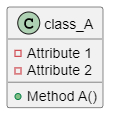
\includegraphics[scale=0.75]{class example from class diagram.png}
            \caption{Contoh dari sebuah \textit{class}}
        \end{figure}
        \item \textit{Attributes}\\
        \textit{Attributes} adalah sebuah properti dari \textit{class} yang berisikan informasi-informasi yang ingin ditangkap. Seperti contoh, nama seseorang beserta dengan umurnya dan alamatnya. \textit{Attributes} ini juga dapat dihitung (\textit{calculated}) ataupun diturunkan (\textit{derived}) ke \textit{attribute} lainnya\autocite{systemanalysisdesign-class-diagram}.
        \textit{Attributes} juga dapat dibagi menjadi tiga jenis berdasarkan visibilitasnya dalam \textit{class diagram}, ketiga jenis tersebut antara lain:
        \begin{itemize}
            \item \textit{Public Attribute}\\
            \textit{Public Attribute} merupakan jenis \textit{attribute} yang tidak disembunyikan dari \textit{class} lainnya (publik). Ini berarti \textit{attribute} jenis ini dapat diakses secara publik dari objek/\textit{class} manapun\autocite{systemanalysisdesign-class-diagram}.
            \item \textit{Protected Atrribute}\\
            \textit{Protected Attribute} merupakan sebuah jenis \textit{attribute} yang disembunyikan dari semua \textit{class} lain kecuali \textit{subclass} dari \textit{class} yang menyimpan attribute tersebut\autocite{systemanalysisdesign-class-diagram}.
            \item \textit{Private Atrribute}\\
            \textit{Private Attribute} merupakan jenis \textit{attribute} yang disembunyikan dari \textit{class} lainnya dan hanya dapat diakses oleh \textit{class} yang menyimpan \textit{attribute} tersebut\autocite{systemanalysisdesign-class-diagram}.
        \end{itemize}
        \item \textit{Operations}\\
        \textit{Operations} atau juga bisa disebut sebagai \textit{method}/(metode), ialah sebuah aksi atau fungsi (\textit{functions}) yang dapat dilakukan oleh \textit{class} tersebut. \textit{Operations} dibagi ke dalam empat jenis yakni, \textit{constructor, query, update} dan \textit{destructor}\autocite{systemanalysisdesign-class-diagram}.
        \begin{itemize}
            \item \textit{Constructor Operation}\\
            \textit{Constructor Operation} merupakan sebuah operasi yang bertugas untuk membuat (\textit{create}) sebuah \textit{instance} dari \textit{class}. Biasanya, \textit{operation} jenis ini tidak secara eksplisit ditampilkan di dalam \textit{class diagram} dikarenakan hanya mengimplementasikan sebuah \textit{function} yang \textit{basic}\autocite{systemanalysisdesign-class-diagram}.
            \item \textit{Query Operation}\\
            \textit{Query Operation} merupakan jenis \textit{operation} yang membuat informasi mengenai \textit{state} (status) dari suatu objek tersedia untuk objek lain tanpa mengubah objek tersebut ke dalam bentuk apapun\autocite{systemanalysisdesign-class-diagram}.
            \item \textit{Update Operation}\\
            \textit{Update Operation} merupakan sebuah jenis operasi yang bertugas untuk mengubah sebuah \textit{value} dari beberapa atau semua atribut objek. Hal ini juga dapat mengakibatkan perubahan dari \textit{state} (status) objek-objek tersebut\autocite{systemanalysisdesign-class-diagram}.
            \item \textit{Destructor Operation}\\
            \textit{Destructor Operation} adalah sebuah jenis \textit{operation} yang bertugas untuk menghapus atau menghilangkan objek dari sistem tersebut\autocite{systemanalysisdesign-class-diagram}.
        \end{itemize}
    \end{itemize}
    Di dalam \textit{class diagram}, sebuah \textit{class} dapat terlibat dalam satu atau lebih hubungan/\textit{relationship} dengan \textit{class} lainnya. Secara garis besar, hubungan-hubungan antarkelas di dalam \textit{class diagram} terbagi sebagai berikut:
    \begin{itemize}
        \item \textit{Association}\\
        \textit{Association} dapat diartikan sebagai hubungan struktural antara dua \textit{class} yang sederajat\autocite{what-is-class-diagram}. Ini menandakan adanya asosiasi/hubungan antara satu \textit{class} dengan satu \textit{class} lain. Salah satu contoh hubungan ini adalah seorang pasien yang menjadwalkan sebuah \textit{appointment}. Hubungan antara \textit{class} 'Pasien' dengan \textit{class} 'Appointment' adalah sebuah \textit{association}\autocite{systemanalysisdesign-class-diagram-relations}.\\
        \textbf{Representasi Grafis}:\\
        \begin{figure}[h]
            \centering
            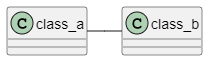
\includegraphics[scale=0.5]{class diagram - association example.png}
            \caption{Contoh dari relasi \textit{Association}}
        \end{figure}
        \item \textit{Generalization (Inheritance)}\\
        \textit{Generalization} merupakan sebuah hubungan yang menggambarkan sebuah \textit{class} yang mewarisi/(\textit{inherit attribute}) atau \textit{operation} dari \textit{class} yang lain\autocite{what-is-class-diagram}. Hubungan jenis ini merepresentasikan sebuah relasi berbentuk \textit{"is-a"} atau \textit{"a-kind-of"} antarkelas. Contoh hubungan ini adalah seperti halnya hubungan antara 'Pelanggan' dan 'Karyawan'. Kedua-duanya merupakan turunan dari \textit{class} 'Orang' atau '\textit{Person}'. \textit{Class} 'Orang' dapat dinamakan sebagai \textit{superclass} karena \textit{class} itulah yang mewarisi kedua \textit{class} lainnya, sedangkan 'Karyawan' dan 'Pelanggan' dapat disebut sebagai sebuah \textit{subclass}, karena kedua \textit{class} tersebut diwarisi oleh sebuah \textit{class} lain\autocite{systemanalysisdesign-class-diagram-relations}.\\
        \textbf{Representasi Grafis}:\\
        \begin{figure}[h]
            \centering
            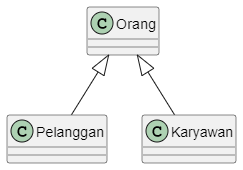
\includegraphics[scale=0.375]{class diagram generalization example.png}
            \caption{Contoh dari relasi \textit{Generalization}}
        \end{figure}
        \item \textit{Aggregation}\\
        \textit{Aggregation} merupakan jenis \textit{association} yang spesial/khusus. Hubungan ini merepresentasikan hubungan \textit{"a-part-of"} atau \textit{"has-parts"}. Contoh nyatanya adalah 'mahasiswa merupakan bagian dari sebuah kelas', 'seorang karyawan merupakan bagian dari sebuah perusahaan' dan 'mesin adalah bagian dari sebuah mobil'. Sama seperti hubungan \textit{Generalization}, hubungan \textit{Aggregation} juga dapat dibentuk menjadi sebuah hirarki\autocite{systemanalysisdesign-class-diagram-relations}.\\
        \textbf{Representasi Grafis}:\\
        \begin{figure}[h]
            \centering
            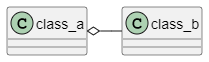
\includegraphics[scale=0.5]{class diagram - aggregation example.png}
            \caption{Contoh dari relasi \textit{Aggregation}}
        \end{figure}

        \item \textit{Composition}

        \textit{Composition} merupakan sebuah hubungan yang mirip dengan \textit{aggregation}. Namun yang membedakannya adalah apabila \textit{superclass}-nya dihancurkan, maka bagian-bagiannya atau dalam kata lain (\textit{subclass}) dari \textit{superclass} itu juga akan hancur. Contohnya adalah kepala, tangan dan kaki merupakan bagian tubuh dari seseorang, apabila orangnya tidak ada, maka kepala, tangan dan kaki orang tersebut juga tidak ada\autocite{what-is-class-diagram}.

        \textbf{Representasi Grafis}:\\
        \begin{figure}[h]
            \centering
            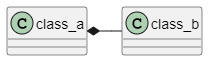
\includegraphics[scale=0.5]{class diagram composition example.png}
            \caption{Contoh dari relasi \textit{Composition}}
        \end{figure}
    \end{itemize}
    \textit{Relationship} juga dapat memiliki \textit{multiplicity}. \textit{Multiplicity} inilah yang mendokumentasikan bagaimana sebuah \textit{instance} dari sebuah objek dapat diasosiasikan dengan \textit{instance} lainnya. \textit{Multiplicity} biasanya dituliskan sebagai angka dalam bentuk format "angka minimum.. angka maksimum"\autocite{systemanalysisdesign-class-diagram}. Berapa banyak objek dari setiap \textit{class} yang mengambil bagian dalam \textit{relationship} dan \textit{multiplicity} dapat dinyatakan sebagai berikut:
    \begin{itemize}
        \item \textit{Exactly One} (1)\\
        \begin{figure}[h]
            \centering
            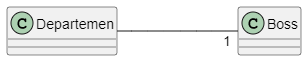
\includegraphics[scale=0.475]{multiplicity exactly one.png}\\
            % Departemen hanya memiliki satu dan hanya satu bos saja.
            \caption{Departemen hanya memiliki satu dan hanya satu bos saja.}
        \end{figure}
        \item \textit{Zero or One} (0.. 1)\\
        \begin{figure}[h]
            \centering
            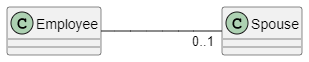
\includegraphics[scale=0.475]{multiplicity zero to one example.png}\\
            % Seorang karyawan dapat menikahi dengan nol atau satu pasangan.
            \caption{Seorang karyawan dapat menikahi dengan nol atau satu pasangan.}
        \end{figure}
        \item \textit{Many} atau \textit{Zero or More} (* atau 0.. *)\\
        \begin{figure}[h]
            \centering
            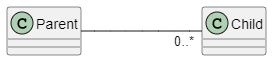
\includegraphics[scale=0.475]{multiplicity many example.png}\\
            % Orang tua dapat memiliki nol hingga banyak anak.
            \caption{Orang tua dapat memiliki nol hingga banyak anak.}
        \end{figure}
        \item \textit{One or More} (1.. *)\\
        \begin{figure}[h]
            \centering
            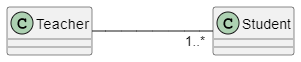
\includegraphics[scale=0.475]{multiplicity one or more example.png}\\
            % Seorang guru dapat memiliki satu atau lebih murid.
            \caption{Seorang guru dapat memiliki satu atau lebih murid.}
        \end{figure}
        \newpage
        \item \textit{Exact Number} atau \textit{Specified Range} (8 atau 2.. 5)\\
        \begin{figure}[h]
            \centering
            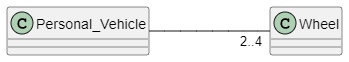
\includegraphics[scale=0.475]{multiplicity specified range example.png}\\
            % Sebuah kendaraan pribadi biasanya hanya memiliki sebanyak dua roda (motor) hingga empat roda (mobil).
            \caption{Sebuah kendaraan pribadi biasanya hanya memiliki sebanyak dua roda (motor) hingga empat roda (mobil).}
        \end{figure}
        \item \textit{Multiple, Disjoint Ranges} (1.. 4, 7)\\
        \begin{figure}[h]
            \centering
            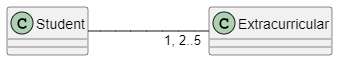
\includegraphics[scale=0.475]{multiplicity multiple disjoint ranges example.png}\\
            % Seorang murid dapat mengikuti satu atau dua hingga lima kegiatan ekstrakulikuler.
            \caption{Seorang murid dapat mengikuti satu atau dua hingga lima kegiatan ekstrakulikuler.}
        \end{figure}
    \end{itemize}
    
    \item \textit{Activity Diagram}\\
    \textit{Acticity Diagram} merupakan salah satu jenis diagram UML yang termasuk ke dalam kelompok \textit{Behavioral Diagrams}. Diagram ini digunakan untuk memodelkan perilaku (\textit{behavior}) di dalam suatu proses bisnis yang tidak tergantung oleh objek. \textit{Activity Diagram} dapat digunakan untuk memodelkan semua jenis proses, dimulai dari alur kerja pada sebuah proses \textit{high-level business} yang melibatkan banyak kasus (\textit{use case}) yang berbeda-beda hingga ke detail dari tiap individual kasus yang ada dan detail yang lebih spesifik pada masing-masing metode yang digunakan\autocite{systemanalysisdesign-activity-diagram}. Berikut adalah notasi-notasi yang digunakan di dalam \textit{activity diagram}:
    \begin{itemize}
        \item \textit{Activity}
        \begin{itemize}
            \item Digunakan sebagai representasi dari serangkian \textit{action}
            \item Dilabelkan sesuai dengan namanya
            \item Digambarkan sebagai sebuah persegi panjang bersudut tumpul\autocite{systemanalysisdesign-activity-diagram}\\
                  Contoh gambar:\\
                  \begin{figure}[h]
                    \centering
                    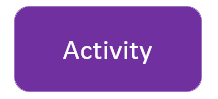
\includegraphics[scale=0.5]{Activity_transparent.png}
                    \caption{Notasi \textit{Activity}}
                  \end{figure}
        \end{itemize}
        \item \textit{Action}
        \begin{itemize}
            \item Merupakan sebuah \textit{behavior} yang sederhana dan tidak dapat diuraikan lagi
            \item Menggambarkan sebuah \textit{task}/tugas yang harus dilakukan\autocite{systemanalysisdesign-activity-diagram}\\
                  Contoh gambar:\\
                  \begin{figure}[h]
                    \centering
                    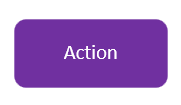
\includegraphics[scale=0.35]{Action_transparent.png}
                    \caption{Notasi \textit{Action}}
                  \end{figure}
        \end{itemize}
        \item \textit{Object Node}
        \begin{itemize}
            \item Digunakan untuk merepresentasikan objek yang terhubung ke sekumpulan aliran objek\autocite{systemanalysisdesign-activity-diagram}\\
                  Contoh gambar:\\
                  \begin{figure}[h]
                    \centering
                    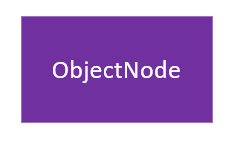
\includegraphics[scale=0.45]{ObjectNode_transparent.png}
                    \caption{Notasi \textit{Object Node}}
                  \end{figure}
        \end{itemize}
        \item \textit{Control Flow}
        \begin{itemize}
            \item Menunjukkan urutan eksekusi di dalam \textit{activity diagram}
            \item Biasanya digambarkan sebagai arah panah\autocite{systemanalysisdesign-activity-diagram}\\
                  Contoh gambar:\\
                  \begin{figure}[h]
                    \centering
                    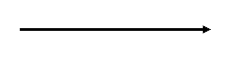
\includegraphics[scale=0.5]{Control Flow_transparent.png}
                    \caption{Notasi \textit{Control Flow}}
                  \end{figure}
        \end{itemize}
        \item \textit{Object Flow}
        \begin{itemize}
            \item Menunjukkan aliran objek dari satu \textit{activity} (atau \textit{action}) ke \textit{activity} (atau \textit{action}) lainnya
            \item Biasanya digambarkan sebagai arah panah dengan garis yang putus-putus\autocite{systemanalysisdesign-activity-diagram}\\
                  Contoh gambar:\\
                  \begin{figure}[h]
                    \centering
                    
\includegraphics[scale=0.5]{Object Flow_transparent.png}
                    \caption{Notasi \textit{Object Flow}}
                  \end{figure}
        \end{itemize}
        \item \textit{Initial Node}
        \begin{itemize}
            \item Menggambarkan awal dari serangkain \textit{activity} atau \textit{action} pada \textit{activity diagram}\autocite{systemanalysisdesign-activity-diagram}\\
                  Contoh gambar:\\
                  \begin{figure}[h]
                    \centering
                    
\includegraphics[scale=0.45]{Initial Node_transparent.png}
                    \caption{Notasi \textit{Initial Node}}
                  \end{figure}
        \end{itemize}
        \newpage
        \item \textit{Final Activity Node}
        \begin{itemize}
            \item Digunakan sebagai tanda untuk memberhentikan semua aliran kontrol dan aliran objek dalam suatu \textit{activity} atau \textit{action}\autocite{systemanalysisdesign-activity-diagram}\\
                  Contoh gambar:\\
                  \begin{figure}[h]
                    \centering
                    
\includegraphics[scale=0.45]{Final Activity Node_transparent.png}
                    \caption{Notasi \textit{Final Activity Node}}
                  \end{figure}
        \end{itemize}
        \item \textit{Final Flow Node}
        \begin{itemize}
            \item Digunakan untuk menghentikan aliran kontrol atau aliran objek tertentu\autocite{systemanalysisdesign-activity-diagram}\\
                  Contoh gambar:\\
                  \begin{figure}[h]
                    \centering
                    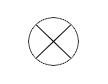
\includegraphics[scale=0.45]{Final flow node_transparent.png}
                    \caption{Notasi \textit{Final Flow Node}}
                  \end{figure}
        \end{itemize}
        \item \textit{Decision Node}
        \begin{itemize}
            \item Digunakan untuk menggambarkan sebuah \textit{test condition} untuk memastikan aliran kontrol atau objek tersebut hanya berjalan pada satu jalur saja
            \item Biasanya diberikan label sesuai dengan kriteria dari keputusan yang dibutuhkan untuk lanjut melewati jalur tertentu\autocite{systemanalysisdesign-activity-diagram}\\
                  Contoh gambar:\\
                  \begin{figure}[h]
                    \centering
                    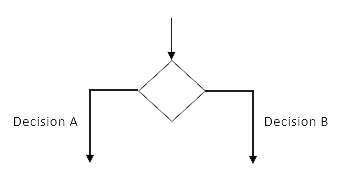
\includegraphics[scale=0.5]{Decision Node_transparent.png}
                    \caption{Notasi \textit{Decision Node}}
                  \end{figure}
        \end{itemize}
        \newpage
        \item \textit{Merge Node}
        \begin{itemize}
            \item Digunakan untuk menyatukan kembali jalur \textit{decision} berbeda yang sebelumnya sudah dibuat menggunakan \textit{Decision Node}\autocite{systemanalysisdesign-activity-diagram}\\
                  Contoh gambar:\\
                  \begin{figure}[h]
                    \centering
                    \includegraphics*[width=4cm]{Merge Node_transparent.png}
                    \caption{Notasi \textit{Merge Node}}
                  \end{figure}
        \end{itemize}
        \item \textit{Fork Node}
        \begin{itemize}
            \item Digunakan untuk membagi \textit{behavior} menjadi sebuah serangkaian \textit{activity} atau \textit{action} yang berjalan secara bersamaan/paralel\autocite{systemanalysisdesign-activity-diagram}\\
                  Contoh gambar:\\
                  \begin{figure}[h]
                    \centering
                    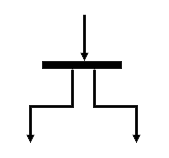
\includegraphics[scale=0.5]{Fork Node_transparent.png}
                    \caption{Notasi \textit{Fork Node}}
                  \end{figure}
        \end{itemize}
        \item \textit{Join Node}
        \begin{itemize}
            \item Digunakan untuk menggabungkan kembali serangkaian \textit{activity} atau \textit{action} yang paralel tersebut\autocite{systemanalysisdesign-activity-diagram}\\
                  Contoh gambar:\\
                  \begin{figure}[h]
                    \centering
                    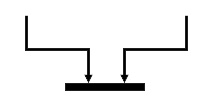
\includegraphics[scale=0.5]{Join Node_transparent.png}
                    \caption{Notasi \textit{Join Node}}
                  \end{figure}
        \end{itemize}
        \item \textit{Swimlane}
        \begin{itemize}
            \item Digunakan untuk memecah \textit{activity diagram} menjadi beberapa baris dan kolom dengan tujuan untuk menentukan masing-masing \textit{activity} atau \textit{action} ke individu atau objek yang bertanggung jawab untuk menjalankan \textit{activity} atau \textit{action}
            \item Biasanya diberikan label yang berisikan nama dari individu atau objek yang bertanggung jawab\autocite{systemanalysisdesign-activity-diagram}\\
                  Contoh gambar:\\
                  \begin{figure}[h]
                    \centering
                    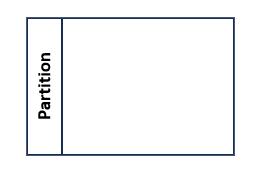
\includegraphics[scale=0.5]{Swimlane_transparent.png}
                    \caption{Notasi \textit{Swimlane}}
                  \end{figure}
        \end{itemize}
    \end{itemize}
    \item \textit{Use-Case Diagram}\\
    \textit{Use-Case Diagram} merupakan salah satu jenis diagram UML yang digunakan untuk menentukan konteks dan \textit{requirements} dari sebuah sistem serta memvalidasi bentuk arsitektur dari sebuah sistem yang digambarkan dengan mengimplementasikan satu atau beberapa \textit{test case}/\textit{use case}\autocite{systemanalysisdesign-use-case-diagram}.
    \begin{figure}[h]
        \centering
        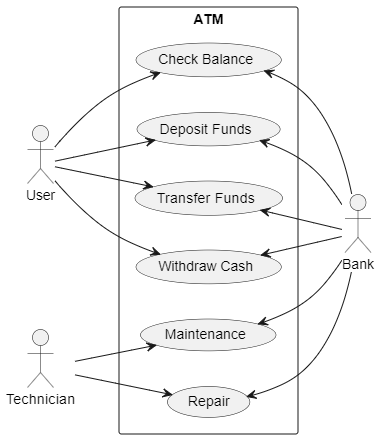
\includegraphics[scale=0.5]{use case diagram simple example.png}
        \caption{Contoh bentuk dari \textit{use-case diagram}}
    \end{figure}\\
    \textit{Use-Case Diagram} biasanya dibuat dan digunakan pada tahap awal \textit{development} suatu aplikasi. Tujuan dari dibuatnya \textit{use-case diagram} antara lain, menentukan konteks pada sebuah sistem, memvalidasi arsitektur dari suatu sistem, menetapkan \textit{requirements} yang dibutuhkan oleh sebuah sistem dan mendorong adanya implementasi dan menghasilkan \textit{test case}/\textit{use case} pada sistem tersebut. Berikut adalah komponen-komponen yang ada pada \textit{Use-Case Diagram}:
    \begin{itemize}
        \item \textit{Actor}\\
        Merupakan sebuah komponen yang menggambarkan 'seseorang' atau sebuah 'sistem' yang memperoleh \textit{benefit} dari \textit{subject} dan berada di luar \textit{subject boundary}. Biasanya digambarkan sebagai sebuah \textit{stick figure} atau sebuah figur bukan manusia lainnya dan diberi label sesuai dengan \textit{role}-nya. \textit{Actor} ini juga dapat di asosiasikan dengan \textit{actor} lainnya melalui asosiasi \textit{specialization/superclass} yang ditandai dengan arah panah dengan mata panah yang berongga (\textit{hollow})\autocite{systemanalysisdesign-use-case-diagram}.
        \begin{figure}[h]
            \centering
            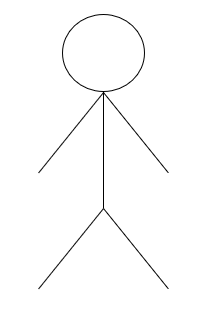
\includegraphics[scale=0.5]{use case - actor.png}
            \caption{Bentuk dari \textit{actor}}
        \end{figure}
        \newpage
        \item \textit{Use Case}\\
        Merupakan sebuah komponen yang menggambarkan bagian utama dari fungsionalitas sistem. \textit{Use Case} ini dapat \textit{extend} ke \textit{use case} lain dan juga dapat \textit{include} \textit{use case} lain. Komponen ini berada di dalam \textit{subject boundary} dan biasanya diberi label sesuai dengan fungsi/\textit{use case} yang ingin di tampilkan\autocite{systemanalysisdesign-use-case-diagram}.
        \begin{figure}[h]
            \centering
            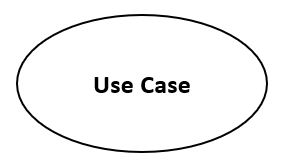
\includegraphics[scale=0.5]{use case - use case.png}
            \caption{Bentuk dari \textit{use case}}
        \end{figure}
        \item \textit{Subject Boundary}\\
        Komponen inilah yang merepresentasikan ruang lingkup \textit{subject} yang ingin ditampilkan (sebuah sistem atau proses bisnis individu)\autocite{systemanalysisdesign-use-case-diagram}.
        \begin{figure}[h]
            \centering
            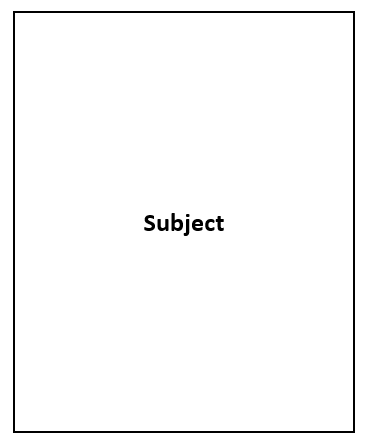
\includegraphics[scale=0.5]{use case - subject boundary.png}
            \caption{Bentuk dari \textit{subject boundary}}
        \end{figure}
        \newpage
        \item \textit{Association Relationship}\\
        Komponen inilah yang menghubungkan \textit{actor} dengan \textit{use case} yang berinteraksi dengannya\autocite{systemanalysisdesign-use-case-diagram}.
        \begin{figure}[h]
            \centering
            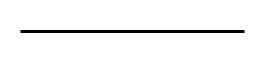
\includegraphics[scale=0.5]{use case - association.png}
            \caption{Bentuk dari \textit{Association Relationship}}
        \end{figure}
        \item \textit{'Include' Relationship}\\
        Merupakan penyertaan fungsionalitas dari satu \textit{use case} di dalam \textit{use case} lainnya\autocite{systemanalysisdesign-use-case-diagram}. Ini menandakan bahwa \textit{use case} yang di-\textit{include}  tersebut bersifat wajib dan merupakan bagian dari \textit{use case} dasarnya. Salah satu contoh kasusnya adalah apabila seseorang ingin membaca buku, maka orang tersebut harus membuka bukunya terlebih dahulu. Ini menandakan bahwa \textit{use case} 'Membaca Buku' meng-\textit{include} \textit{use case} 'Membuka Buku', karena, apabila seseorang ingin membaca buku, maka sudah pasti buku tersebut harus dibuka terlebih dahulu\autocite{educativeio-include-extend-usecase}.
        \begin{figure}[h]
            \centering
            
\includegraphics[scale=0.5]{use case - include.png}
            \caption{Bentuk dari \textit{Include Relationship}}
        \end{figure}
        \newpage
        \item \textit{'Extends' Relationship}\\
        Merupakan sebuah ekstensi dari use case untuk menyertakan suatu \textit{behavior} yang opsional\autocite{systemanalysisdesign-use-case-diagram}.
        \begin{figure}[h]
            \centering
            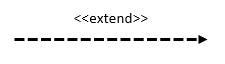
\includegraphics[scale=0.5]{use case - extend.png}
            \caption{Bentuk dari \textit{Extend Relationship}}
        \end{figure}
        \item \textit{Generalization Relationship}\\
        Mewakili sebuah penggunaan \textit{use case} khusus ke \textit{use case} yang lebih umum\autocite{systemanalysisdesign-use-case-diagram}. Relasi \textit{generalization} adalah hubungan \textit{parent-child} antar-\textit{use case}\autocite{what-is-usecase-diagram}.
        \begin{figure}[h]
            \centering
            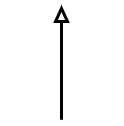
\includegraphics[scale=0.5]{use case - generalization.png}
            \caption{Bentuk dari \textit{Generalization Relationship}}
        \end{figure}
    \end{itemize}
    \item \textit{Sequence Diagram}\\
    \textit{Sequence Diagram} merupakan sebuah jenis \textit{interaction diagram} yang menjelaskan detail bagaimana sebuah operasi dilakukan. Diagram ini menangkap interaksi antar objek dalam konteks kolaborasi. \textit{Sequence Diagram} berfokus pada waktu dan menunjukkan urutan interaksi secara visual dengan menggunakan sumbu vertikal diagram untuk merepresentasikan waktu, pesan apa yang dikirim dan kapan\autocite{what-is-sequence-diagram}.
    
    \begin{figure}[h]
        \centering
        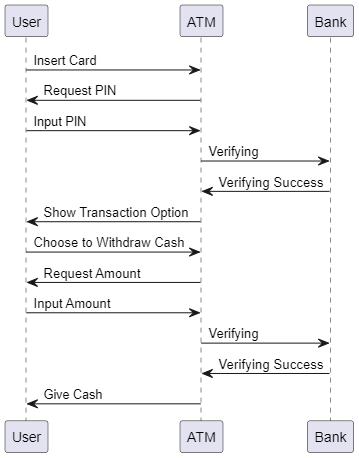
\includegraphics[width=6cm,height=4cm]{sequence diagram simple example.png}
        \caption{Contoh sederhana dari \textit{Sequence Diagram} dalam kasus penarikan tunai di ATM}
    \end{figure}
    \newpage
    Berikut adalah komponen-komponen yang ada pada \textit{Sequence Diagram}:
    
    \begin{itemize}
        \item \textit{Actor}\\
        Merupakan komponen yang menggambarkan 'seseorang' atau 'sistem' memperoleh \textit{benefit} dari dan berada di luar sistem tersebut. \textit{Actor} ini ikut berpartisipasi dalam \textit{sequence} dengan mengirim dan/atau menerima \textit{message} dan biasanya \textit{actor} tersebut diletakkan di bagian teratas pada diagram\autocite{systemanalysisdesign-sequence-diagram}.
        \begin{figure}[h]
            \centering
            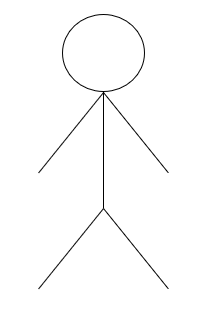
\includegraphics[scale=0.5]{use case - actor.png}
            \caption{Bentuk dari \textit{actor}}
        \end{figure}
        \item \textit{Object}\\
        Merupakan sebuah objek yang ikut berpartisipasi di dalam \textit{sequence} dengan mengirim dan/atau menerima \textit{message}. Biasanya juga diletakkan di bagian teratas diagram seperti layaknya \textit{actor}\autocite{systemanalysisdesign-sequence-diagram}.
        \begin{figure}[h]
            \centering
            
\includegraphics[scale=0.5]{sequence - object.png}
            \caption{Bentuk dari \textit{object}}
        \end{figure}
        \item \textit{Lifeline}\\
        Komponen yang menunjukkan masa waktu hidup suatu objek di dalam \textit{sequence}\autocite{systemanalysisdesign-sequence-diagram}.
        \begin{figure}[h]
            \centering
            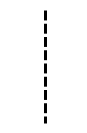
\includegraphics[scale=0.5]{sequence - lifeline.png}
            \caption{Bentuk dari \textit{lifeline}}
        \end{figure}
        \item \textit{Execution Occurrence}\\
        Merupakan sebuah persegi panjang yang ditempatkan di atas sejajar dengan \textit{lifeline} yang menandakan kapan suatu objek mengirim atau menerima \textit{message}\autocite{systemanalysisdesign-sequence-diagram}.
        \begin{figure}[h]
            \centering
            
\includegraphics[scale=0.5]{sequence - execution occurrence.png}
            \caption{Bentuk dari \textit{execution occurrence}}
        \end{figure}
        \item \textit{Message}\\
        Berguna untuk menyampaikan informasi dari satu objek ke objek lainnya\autocite{systemanalysisdesign-sequence-diagram}.
        \begin{figure}[h]
            \centering
            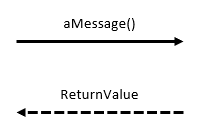
\includegraphics[scale=0.5]{sequence - message.png}
            \caption{Bentuk dari \textit{message}}
        \end{figure}
        \item \textit{Guard Condition}\\
        Komponen ini yang mewakili pengujian yang harus dipenuhi agar pesan dapat dikirim\autocite{systemanalysisdesign-sequence-diagram}.
        \begin{figure}[h]
            \centering
            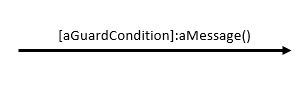
\includegraphics[width=6cm,height=1cm]{sequence - guard condition.png}
            \caption{Bentuk dari \textit{guard condition}}
        \end{figure}
        \newpage
        \item \textit{Object Destruction}\\
        Sebuah tanda "X" ditempatkan di akhir \textit{lifeline} suatu objek untuk menunjukkan bahwa objek tersebut akan hilang\autocite{systemanalysisdesign-sequence-diagram}.
        \begin{figure}[h]
            \centering
            
\includegraphics[width=1cm,height=1cm]{sequence - object destruction.png}
            \caption{Bentuk dari \textit{object destruction}}
        \end{figure}
        \item \textit{Frame}\\
        Menunjukkan konteks \textit{sequence diagram}\autocite{systemanalysisdesign-sequence-diagram}.
        \begin{figure}[h]
            \centering
            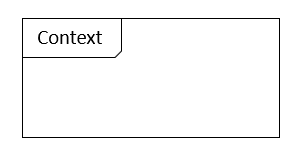
\includegraphics[scale=0.45]{sequence - frame.png}
            \caption{Bentuk dari \textit{frame}}
        \end{figure}
    \end{itemize}
\end{enumerate}
\subbab{Aplikasi Serupa}
Berikut adalah beberapa aplikasi sejenis yang sudah pernah dikembangkan atau dibuat oleh beberapa penelitian terdahulu:

\begin{itemize}
    \item Aplikasi \textit{marketplace} untuk produk agrikultural
    
    Sebuah aplikasi berbasis \textit{mobile} yang dikembangkan oleh Heru Nugroho, Robbi Hendriyanto dan Kautsar Tisamawi. Aplikasi ini dibuat dengan tujuan untuk membantu para petani di Indonesia memperdagangkan produk-produk agrikultur yang telah mereka panen ke masyarakat dengan harga yang sewajarnya\autocite{agriculture-marketplace}. 

    \item Aplikasi bernama e-Nelayan yang menjual ikan
    
    Aplikasi berbasis \textit{mobile} yang dikembangkan untuk membantu para nelayan di Kota Samarahan, Malaysia untuk memperdagangkan hasil tangkapan ikan mereka ke para pedagang/pasar dan/atau kepada warga secara langsung. Aplikasi ini dikembangkan oleh Mohammad Nazrul Mornie, Nurfauza Jali, Kartinah Zen dan Suriati Khartini Jali\autocite{fishes-marketplace}.

    \item Aplikasi perdagangan ikan C2C menggunakan metode \textit{SMS Gateway}
    
    Sebuah aplikasi berbasis \textit{mobile} dan web yang dikembangkan untuk membantu para nelayan di wilayah pedalaman Pulau Batam untuk mendagangkan ikan-ikan mereka kepada masyarakat dengan menggunakan metode \textit{SMS Gateway}. Aplikasi ini dikembangkan oleh Dwi Ely Kurniawan, Nur Zahrati Janah, Ari Wibowo, Mir'atul Khusna Mufida dan Purwono Prasetyawan\autocite{c2c-fish-marketplace}.

    \item Aplikasi rental mobil bernama LIDI
    
    Aplikasi berbasis web yang dikembangkan dengan tujuan untuk membantu para usaha penyewa mobil untuk menyewakan mobil-mobil mereka kepada warga di wilayah Sidoarjo secara \textit{online}. Aplikasi ini dikembangkan oleh N F Rozi, M Ruswiansari, A Rachman, S R Wardhana dan L Istiyanto\autocite{lidi-car-rental}. 

    \item Aplikasi \textit{e-marketplace} untuk badan usaha kecil, mikro dan menengah milik desa
    
    Aplikasi berbasis web yang ditujukan kepada Badan Usaha Milik (BUM) Desa Pakis Sabilulungan di wilayah Mekarsari, Bandung, Indonesia. Aplikasi ini dikembangkan oleh Rachmadita Andreswari bersama dengan Nia Ambarsari, Alvi Syahrina, Warih Puspitasari, Atik Novianti dan Irfan Darmawan\autocite{bum-mekarsari}.

\end{itemize}

\newpage
\bab{Bab 3. Metode Penelitian}
\subbab{Metode Penelitian}
Metode penelitian yang digunakan dalam penulisan penelitian ini terfokus pada pengumpulan data yang diperlukan. Data tersebut dikumpulkan dengan cara melakukan survei yang dibuka ke publik yang diisi oleh 122 orang, selain itu juga dilakukan studi pustaka menggunakan \textit{paper} yang berusia dibawah lima tahun, buku yang dibawah 10 tahun dan dokumen-dokumen yang ditemukan di internet. Adapula tahapan kerangka berfikir yang dilakukan dalam penelitian ini yang dapat dilihat pada gambar \ref{fig:KerangkaBerfikir}.

\begin{figure}[h]
    \centering
    \includegraphics*[width=10cm]{./images/Kerangka Berfikir.png}
    \caption{Kerangka Berfikir}
    \label{fig:KerangkaBerfikir}
\end{figure}

Pengembangan \textit{website shumishumi} ini menggunakan metode \textit{agile scrum}, metode pengembangan \textit{software} ini sudah diejlaskan dengan detail di Bab 2. Sedangkan struktur \textit{scrum} yang dilakukan saat mengembangkan \textit{website} ini adalah
\begin{enumerate}
    \item \textit{Backlog Grooming}
    Tahapan \textit{backlog grooming} atau \textit{Backlog refinement} dilakukan untuk memastikan semua \textit{stories} yang ada didalam \textit{backlog} sesuai dengan \textit{requirement} yang didapat dan dalam tahapan ini juga \textit{user stories} akan dipecah menjadi \textit{task-task} yang lebih kecil dan diberi \textit{story points}(satu \textit{story point} sama dengan tiga jam) berdasarkan \textit{effort} yang dibutuhkan untuk mengerjakan \textit{task} tersebut.

\begin{longtable}{@{}|l|l|l|l|@{}}
\toprule
\textit{User Stories} & \textit{Task} & \textit{Priority} & \textit{Story Point} \\* \midrule
\endfirsthead
\centering
%
\endhead
%
\multirow{5}{*}{\textit{Project Initialization}} & \textit{Initialize NextJS FrontEnd Project} & \textit{P0} & \textit{5 SP} \\* \cmidrule(l){2-4}
 & \textit{Initialize Springboot BackEnd Project} & \textit{P0} & \textit{5 SP} \\* \cmidrule(l){2-4}
 & \textit{Create Database Structure} & \textit{P0} & \textit{3 SP} \\* \cmidrule(l){2-4}
 & \textit{Connect BE to Database} & \textit{P0} & \textit{2 SP} \\* \cmidrule(l){2-4}
 & \textit{Create CORS Configuration for BE} & \textit{P0} & \textit{2 SP} \\* \midrule
\multirow{2}{*}{\textit{\begin{tabular}[c]{@{}l@{}}User can upload \\ and download image\end{tabular}}} & \textit{{[}BE{]} Create image download API} & \textit{P0} & \textit{3 SP} \\* \cmidrule(l){2-4}
 & \textit{{[}BE{]} Create image upload API} & \textit{P0} & \textit{3 SP} \\* \midrule
\multirow{9}{*}{\textit{User can manage account}} & \textit{{[}BE{]} Create register API} & \textit{P0} & \textit{3 SP} \\* \cmidrule(l){2-4}
 & \textit{{[}BE{]} Create user info API} & \textit{P0} & \textit{3 SP} \\* \cmidrule(l){2-4}
 & \textit{{[}BE{]} Create user update API} & \textit{P1} & \textit{3 SP} \\* \cmidrule(l){2-4}
 & \textit{{[}BE{]} Create merchant apply API} & \textit{P1} & \textit{3 SP} \\* \cmidrule(l){2-4}
 & \textit{{[}FE{]} Create register page} & \textit{P0} & \textit{3 SP} \\* \cmidrule(l){2-4}
 & \textit{{[}FE{]} Create home page} & \textit{P0} & \textit{5 SP} \\* \cmidrule(l){2-4}
 & \textit{{[}FE{]} Create User Info page} & \textit{P1} & \textit{3 SP} \\* \cmidrule(l){2-4}
 & \textit{{[}FE{]} Create User update page} & \textit{P1} & \textit{5 SP} \\* \cmidrule(l){2-4}
 & \textit{{[}FE{]} Create apply to merchant button} & \textit{P1} & \textit{1 SP} \\* \midrule
\multirow{4}{*}{\textit{User can manage session}} & \textit{{[}FE{]} Create login page} & \textit{P0} & \textit{4 SP} \\* \cmidrule(l){2-4}
 & \textit{{[}FE{]} Create logout button} & \textit{P0} & \textit{2 SP} \\* \cmidrule(l){2-4}
 & \textit{{[}BE{]} Create login API} & \textit{P0} & \textit{3 SP} \\* \cmidrule(l){2-4}
 & \textit{{[}BE{]} Create logout API} & \textit{P0} & \textit{3 SP} \\* \midrule
\multirow{8}{*}{\textit{\begin{tabular}[c]{@{}l@{}}User can browse item and \\ Get recommendation \\ base on their activities\end{tabular}}} & \textit{{[}BE{]} Create item query list API} & \textit{P0} & \textit{3 SP} \\* \cmidrule(l){2-4}
 & \textit{{[}BE{]} Create item filter API} & \textit{P0} & \textit{3 SP} \\* \cmidrule(l){2-4}
 & \textit{{[}BE{]} Create item info API} & \textit{P0} & \textit{3 SP} \\* \cmidrule(l){2-4}
 & \textit{\begin{tabular}[c]{@{}l@{}}{[}BE{]} Create new table for \\ knowledge graph calculation\end{tabular}} & \textit{P0} & \textit{2 SP} \\* \cmidrule(l){2-4}
 & \textit{{[}BE{]} Create GetRecommendation API} & \textit{P0} & \textit{5 SP} \\* \cmidrule(l){2-4}
 & \textit{\begin{tabular}[c]{@{}l@{}}{[}FE{]} Add recommendation \\ widget in homepage\end{tabular}} & \textit{P0} & \textit{3 SP} \\* \cmidrule(l){2-4}
 & \textit{{[}FE{]} Create search page} & \textit{P0} & \textit{5 SP} \\* \cmidrule(l){2-4}
 & \textit{{[}FE{]} Create item detail page} & \textit{P0} & \textit{3 SP} \\* \midrule
\multirow{4}{*}{\textit{\begin{tabular}[c]{@{}l@{}}User can discuss with \\ other user and merchant\end{tabular}}} & \textit{{[}BE{]} Create discussion create API} & \textit{P2} & \textit{3 SP} \\* \cmidrule(l){2-4}
 & \textit{{[}BE{]} Create edit discussion API} & \textit{P2} & \textit{3 SP} \\* \cmidrule(l){2-4}
 & \textit{{[}BE{]} Create delete discussion API} & \textit{P2} & \textit{3 SP} \\* \cmidrule(l){2-4}
 & \textit{\begin{tabular}[c]{@{}l@{}}{[}FE{]} Add widget for discussion \\ in item detail page\end{tabular}} & \textit{P2} & \textit{2 SP} \\* \midrule
\multirow{5}{*}{\textit{User can manage wishlist}} & \textit{{[}BE{]} Create add to wishlist API} & \textit{P1} & \textit{2 SP} \\* \cmidrule(l){2-4}
 & \textit{{[}BE{]} Create remove from wishlist API} & \textit{P1} & \textit{2 SP} \\* \cmidrule(l){2-4}
 & \textit{{[}BE{]} Create query wishlist API} & \textit{P1} & \textit{3 SP} \\* \cmidrule(l){2-4}
 & \textit{\begin{tabular}[c]{@{}l@{}}{[}FE{]} Create add to wishlist button in \\ Item widget and item detail page\end{tabular}} & \textit{P1} & \textit{1 SP} \\* \cmidrule(l){2-4}
 & \textit{{[}FE{]} Create wishlist page} & \textit{P1} & \textit{3 SP} \\* \midrule
\multirow{5}{*}{\textit{User can manage cart}} & \textit{{[}BE{]} Create add to cart API} & \textit{P0} & \textit{2 SP} \\* \cmidrule(l){2-4}
 & \textit{{[}BE{]} Create update cart API} & \textit{P0} & \textit{2 SP} \\* \cmidrule(l){2-4}
 & \textit{{[}BE{]} Create query cart API} & \textit{P0} & \textit{2 SP} \\* \cmidrule(l){2-4}
 & \textit{\begin{tabular}[c]{@{}l@{}}{[}FE{]} Create add to cart \\ button in item detail page\end{tabular}} & \textit{P1} & \textit{1 SP} \\* \cmidrule(l){2-4}
 & \textit{{[}FE{]} Create cart page} & \textit{P1} & \textit{3 SP} \\* \midrule
\multirow{9}{*}{\textit{User can do transaction}} & \textit{{[}BE{]} Integrate with midtrans for payment} & \textit{P0} & \textit{2 SP} \\* \cmidrule(l){2-4}
 & \textit{{[}BE{]} Create Transaction Create API} & \textit{P1} & \textit{2 SP} \\* \cmidrule(l){2-4}
 & \textit{{[}BE{]} Create Transaction Cancel API} & \textit{P1} & \textit{1 SP} \\* \cmidrule(l){2-4}
 & \textit{{[}BE{]} Create Transaction Finish API} & \textit{P1} & \textit{1 SP} \\* \cmidrule(l){2-4}
 & \textit{{[}BE{]} Create Transaction Query API} & \textit{P1} & \textit{2 SP} \\* \cmidrule(l){2-4}
 & \textit{{[}FE{]} Create Transaction list page} & \textit{P1} & \textit{2 SP} \\* \cmidrule(l){2-4}
 & \textit{{[}FE{]} Create Transaction pay page} & \textit{P1} & \textit{2 SP} \\* \cmidrule(l){2-4}
 & \textit{{[}FE{]} Create Transaction detail page} & \textit{P1} & \textit{2 SP} \\* \cmidrule(l){2-4}
 & \textit{{[}FE{]} Add “Pay” Button in cart page} & \textit{P1} & \textit{1 SP} \\* \midrule
\multirow{5}{*}{\textit{\begin{tabular}[c]{@{}l@{}}User can create review \\ and view existing review\end{tabular}}} & \textit{{[}BE{]} Create API for creating review} & \textit{P2} & \textit{2 SP} \\* \cmidrule(l){2-4}
 & \textit{{[}BE{]} Create API for query review} & \textit{P2} & \textit{2 SP} \\* \cmidrule(l){2-4}
 & \textit{{[}FE{]} Create page for create review} & \textit{P2} & \textit{3 SP} \\* \cmidrule(l){2-4}
 & \textit{{[}FE{]} Create page for merchant review} & \textit{P2} & \textit{2 SP} \\* \cmidrule(l){2-4}
 & \textit{{[}FE{]} Create page for existing user review} & \textit{P2} & \textit{2 SP} \\* \midrule
\multirow{8}{*}{\textit{\begin{tabular}[c]{@{}l@{}}Merchant can \\ manage their item\end{tabular}}} & \textit{{[}BE{]} Create API for create new item} & \textit{P1} & \textit{3 SP} \\* \cmidrule(l){2-4}
 & \textit{{[}BE{]} Create API for update item information} & \textit{P1} & \textit{3 SP} \\* \cmidrule(l){2-4}
 & \textit{{[}BE{]} Create API for delete item} & \textit{P1} & \textit{3 SP} \\* \cmidrule(l){2-4}
 & \textit{{[}FE{]} Create page for create item} & \textit{P1} & \textit{3 SP} \\* \cmidrule(l){2-4}
 & \textit{{[}FE{]} Create page for update item} & \textit{P1} & \textit{3 SP} \\* \cmidrule(l){2-4}
 & \textit{\begin{tabular}[c]{@{}l@{}}{[}FE{]} Create button for create \\ item in merchant page\end{tabular}} & \textit{P2} & \textit{1 SP} \\* \cmidrule(l){2-4}
 & \textit{\begin{tabular}[c]{@{}l@{}}{[}FE{]} Create button for edit item \\ in item detail page\end{tabular}} & \textit{P2} & \textit{1 SP} \\* \cmidrule(l){2-4}
 & \textit{\begin{tabular}[c]{@{}l@{}}{[}FE{]} Create button for delete item \\ in item detail page\end{tabular}} & \textit{P2} & \textit{1 SP} \\* \bottomrule
\caption{\textit{Table backlog}}
\label{tab:my-table}\\
\end{longtable}

    \newpage
    \item \textit{Sprint Planning}

    Kegiatan ini dilakukan untuk mendefinisikan "\textit{scope}" atau batasan-batasan \textit{user stories} yang akan dikerjakan oleh tim \textit{development} di \textit{sprint} yang akan datang, hal ini dilakukan agar semua \textit{task} dapat diselesaikan dalam jangka \textit{sprint} yang telah ditentukan yaitu dua minggu.
    \item \textit{Sprint}

    Pada tahapan ini tim \textit{development} akan mengerjakan sprint backlog seperti yang telah direncanakan di fase sebelumnya, dalam tahmtahapan ini juga dilaksanakan \textit{daily scrum} atau \textit{meeting} yang dilaksanakan untuk mengetahui apakah ada \textit{blocker} atau masalah yangterjadi saat masa \textit{development}.

    \item \textit{Testing}

    Setelah \textit{sprint} selesai, fase \textit{testing} akan dilakukan, \textit{testing} ini akan dilakukan menggunakan \textit{testcase}-\textit{testcase} yang sesuai dengan \textit{task-task} yang dikerjakan di fase \textit{sprint}.

    \item \textit{Sprint Review}

    \textit{Sprint review} ini dilakukan pada akhir \textit{sprint} untuk melaporkan \textit{task-task} atau \textit{user stories} yang sudah dikerjakan di-\textit{sprint} tersebut.
\end{enumerate}

\begin{figure}[h]
    \centering
    \includegraphics*[width=10cm]{./images/gantt1/sprint timeline.png}
    \includegraphics*[width=10cm]{./images/gantt1/sprint timeline 2.png}
    \caption{\textit{Gantt Diagram}}
\end{figure}

\subbab{Analisis}
\subsubbab{Analisis sistem yang sudah berjalan atau perbandingan aplikasi sejenis}

Konsep pengembangan aplikasi \textit{online marketplace} seperti ShumiShumi ini bukanlah yang pertama kali dibuat ataupun dikembangkan. Sebelumnya, sudah ada beberapa penelitian yang serupa yang telah mencoba untuk membuat dan mengembangkan sebuah aplikasi yang sejenis. Berikut adalah perbandingan antara aplikasi ShumiShumi dengan lima penelitian terdahulu yang telah mencoba untuk mengembangkan aplikasi \textit{online marketplace} yang sejenis.

\begin{enumerate}
    \item Aplikasi \textit{marketplace} berbasis \textit{mobile} untuk produk-produk agrikultur

    Penelitian pertama yang akan dibahas adalah sebuah penelitian yang mengembangkan aplikasi \textit{marketplace} berbasis \textit{mobile} untuk produk-produk agrikultur yang dikembangkan oleh Heru Nugroho, Robbi Hendriyanto dan Kautsar Tisamawi. Aplikasi ini merupakan sebuah aplikasi berbasis \textit{mobile} yang dipergunakan untuk menjualbelikan produk-produk yang berhubungan dengan agrikultur seperti padi, jagung, singkong, kentang, buah-buahan, sayur-sayuran dan masih banyak lagi. Aplikasi ini dibuat dengan tujuan untuk membantu para petani di Indonesia untuk menjualbelikan produk-produk agrikultur yang telah mereka panen ke masyarakat dengan harga yang sepadan atau sewajarnya. Dikarenakan sebelumnya, para petani harus melewati rantai perdagangan penjualan produk yang cukup panjang agar produk agrikultur mereka bisa sampai ke masyarakat\autocite{agriculture-marketplace}.

    Rantai perdagangan tersebut dapat meliputi petani itu sendiri, pedagang grosir kecil, pedagang grosir besar, pasar induk, pasar tradisional, dan seterusnya hingga baru sampai ke tangan masyarakat. Hal ini juga menyebabkan harga produk-produk agrikultur yang terjual ke masyarakat menjadi cukup tinggi, sedangkan harga awal yang diberikan oleh petani kepada para pedagang tersebut jauh lebih rendah. Untuk itu, dibuatlah aplikasi \textit{marketplace} agrikultur ini supaya dapat membantu para petani menjualbelikan produk mereka ke masyarakat dengan lebih mudah\autocite{agriculture-marketplace}.

    Aplikasi ini dikembangkan menggunakan \textit{Android Studio} versi 2.2.3 bersama dengan bahasa pemrograman Java dan XML serta menggunakan \textit{framework} bernama CodeIgniter untuk bisa menghubungkan antara \textit{Android} dengan database MySQL yang mereka gunakan\autocite{agriculture-marketplace}.

    \newpage
    Berikut adalah beberapa \textit{screenshot} untuk tampilan UI (\textit{user interface}) dari aplikasi ini:
    \begin{figure}[h]
        \centering
        \includegraphics*[height=6cm,width=0.27\textwidth]{ui app sejenis/Agrikultur Cart - USER.png}\hfill
        \includegraphics*[height=6cm,width=0.27\textwidth]{ui app sejenis/Agrikultur Home Page - USER.png}\hfill
        \includegraphics*[height=6cm,width=0.27\textwidth]{ui app sejenis/Agrikultur Transaksi - USER.png}
        \caption{Beberapa tampilan UI dari sudut pandang pengguna pada aplikasi agrikultur}
    \end{figure}

    Ada beberapa perbedaan yang dapat diamati antara aplikasi \textit{ShumiShumi} dengan aplikasi jual beli produk agrikultur tersebut, walaupun kedua-duanya sama berupaka sebuah aplikasi \textit{maeketplace}. Perbedaan-perbedaan tersebut antara lain sebagai berikut:

    \begin{itemize}
        \item \textit{Platform}

        Perbedaan pertama dapat dilihat dari \textit{platform} tempat aplikasi tersebut ditujukan. Aplikasi penjualan produk agrikultur ini merupakan aplikasi \textit{marketplace} berbasis \textit{mobile}. Yang berarti hanya dapat digunakan pada perangkat berupa \textit{smartphone}. Terlebih lagi aplikasi ini hanya dapat berjalan pada \textit{smartphone} yang memiliki sistem operasi berupa \textit{Android} dikarenakan proses pengembangan sistemnya yang menggunakan \textit{Android Studio}\autocite{agriculture-marketplace}.

        Sedangkan, aplikasi \textit{ShumiShumi} merupakan aplikasi berbasis web, yang berarti perangkat apapun bisa menjalankan aplikasi ini, selama perangkat-perangkat tersebut mempunyai akses untuk internet dan memiliki \textit{web browser}.

        \item Kegunaan dan Ruang Lingkup Aplikasi

        Kegunaan dari aplikasi \textit{ShumiShumi} adalah untuk menjual belikan berbagai macam produk yang berhubungan dengan hobi. Sedangkan aplikasi agrikultur ini, sesuai dengan namanya, yakni menjual berbagai macam barang-barang kebutuhan agrikultur seperti padi, jangung, kentang, dan produk-produk sejenis lainnya\autocite{agriculture-marketplace}.

        \item Fitur-fitur implementasi

        Dari segi fitur implementasi, ternyata kedua aplikasi ini memiliki banyak persamaan. Mulai dari fitur untuk merubah peran/\textit{role} pengguna menjadi penjual apabila pengguna juga ingin menjual produk-produk yang mereka miliki, fitur pencarian hingga fitur pembayaran yang sudah terintegrasi dengan bank-bank lokal.

        Tetapi, banyak juga perbedaan yang dapat diamati dari kedua aplikasi ini antara lain:

        \begin{itemize}
            \item Adanya fitur rekomendasi yang hanya dimiliki oleh aplikasi \textit{ShumiShumi} yang tidak dimiliki oleh aplikasi jual-beli agrikultur tersebut
            \item Fitur \textit{request} yang hanya imiliki oleh aplikasi agrikultur yang dapat membantu pengguna untuk meminta kepada penjual untuk menjual produk-produk yang diinginkan oleh pengguna yang belum ada di dalam aplikasi\autocite{agriculture-marketplace}
            \item Fitur \textit{offer} yang hanya dimiliki aplikasi jual-beli produk agrikultur yang dapat membantu para penjual mempromosikan barang-barang dagangannya secara langsung kepada penggunanya masing-masing. Para pengguna dapat menerima penawaran yang ditawarkan oleh penjual tersebut ataupun menolak tawaran tersebut\autocite{agriculture-marketplace}.
            \item Fitur percakapan diskusi yang hanya dimiliki oleh aplikasi \textit{ShumiShumi} yang dapat membantu penggunanya untuk berdiskusi dengan pengguna lain ataupun dengan penjualnya mengenai barang kebutuhan hobi yang diinginkannya.
        \end{itemize}
    \end{itemize}

    \item Aplikasi bernama \textbf{e-Nelayan} yang menjual produk-produk berupa ikan

    Penelitian kedua merupakan penelitian yang mengembangkan sebuah aplikasi \textit{marketplace} berbasis \textit{mobile} yang menjual belikan produk-produk berupa ikan. Aplikasi ini dikembangkan oleh Mohammad Nazrul Mornie, Nurfauza Jali, Kartinah Zen dan Suriati Khartini Jali. Aplikasi ini berfokus untuk membantu para nelayan terutama di Kota Samarahan, Malaysia untuk menjual ikan-ikan mereka kepada masyarakat dan kepada para pedagang pasar atau penjual ikan\autocite{fishes-marketplace}.

    Aplikasi ini berperan sebagai sebuah \textit{marketplace} bagi komunitas pengguna nelayan, pedagang dan konsumen. Di aplikasi e-Nelayan ini, para nelayan dapat menampilkan hasil tangkapan mereka dan menetapkan harga ikan yang berbeda-beda sesuai dengan hasil tangkapannya. Untuk para pedagang atau penjual ikan yang telah membeli ikan tersebut dari nelayan, mereka dapat memberikan dua opsi pembelian untuk para konsumennya, yakni \textit{self pick-up} (ambil sendiri) atau \textit{cash on delivery} (pembayaran langsung setelah produk dikirim ke konsumen). Terakhir, para konsumen juga dapat meminta \textit{request} kepada pedagang atau nelayan untuk membeli jenis ikan tertentu, yang kemudian dapat dikomentari oleh penjual atau nelayan itu sendiri\autocite{fishes-marketplace}.

    Aplikasi ini dikembangkan menggunakan \textit{Android Studio} dan untuk sistem \textit{database} yang digunakan adalah \textit{Firebase}. Lebih tepatnya adalah \textit{Firebase Realtime Database}, \textit{Firebase Storage}, dan \textit{Firebase Authentication}. \textit{Firebase Realtime Database} digunakan untuk menyimpan semua jenis data yang aplikasi tersebut butuhkan, \textit{Firebase Storage} digunakan untuk menyimpan data yang berupa gambar (terutama gambar profil dan gambar produk), sedangkan \textit{Firebase Authentication} digunakan untuk menyimpan kredensial pengguna bergantung pada jenis autentikasi yang dipilih. Pada aplikasi ini, mereka menggunakan sistem autentikasi berupa \textit{email} dan \textit{password}\autocite{fishes-marketplace}.

    Berikut adalah beberapa \textit{screenshot} untuk tampilan UI (\textit{user interface}) dari aplikasi ini:
    \begin{figure}[h]
        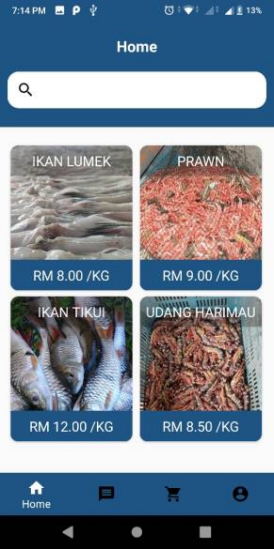
\includegraphics[width=0.27\textwidth]{ui app sejenis/e-Nelayan Home Page.png}\hfill
        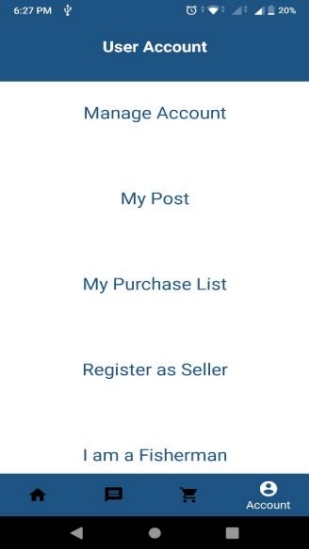
\includegraphics[width=0.27\textwidth]{ui app sejenis/e-Nelayan Account Page.png}\hfill
        \includegraphics[width=0.27\textwidth]{ui app sejenis/e-Nelayan Customer Purchase List.png}
        \caption{Beberapa tampilan UI pada aplikasi e-Nelayan}
    \end{figure}

    Berikut adalah perbedaan-perbedaan yang dimiliki antara aplikasi e-Nelayan dengan aplikasi \textit{ShumiShumi}:

    \begin{itemize}
        \item \textit{Platform}

        Perbedaan pertama dapat dlihat dari \textit{platform} tempat aplikasi ini akan berjalan. Aplikasi e-Nelayahn tersebut merupakan aplikasi berbasis \textit{mobile}, yang berarti hanya dapat berjalan pada perangkat seluler seperti \textit{smartphone}. Terlebih lagi, hanya \textit{smartphone} yang memiliki sistem operasi \textit{Android} saja yang bisa menjalankannya. Dikarenakan pengembangan sistem ini yang hanya menggunakan \textit{Android Studio}\autocite{fishes-marketplace}.

        Sedangkan aplikasi \textit{ShumiShumi} merupakan sebuah aplikasi berbasis web. Yang artinya, dapat digunakan pada perangkat apa saja denagn jenis sistem operasi apa saja selama perangkat-perangkat tersebut memiliki konekasi internet dan \textit{web browser}.

        \item Kegunaan dan Ruang Lingkup Aplikasi

        Perbedaan kedua adalah pada kegunaan dan ruan lingkup aplikasinya. Aplikasi e-Nelayan hanya digunakan untuk membantu proses jual-beli produk-produk berupa ikan dari nelayan ke masyarakat dan hanya diperuntukkan kepada para nelayan, pedagang atau penjual ikan dan para konsumen di wilayah Kota Samarahan, Malaysia\autocite{fishes-marketplace}.

        Sedangkan aplikasi \textit{ShumiShumi} dipergunakan untuk membantu proses jual-beli barang-barang kebutuhan hobi. Mulai dari hobi berolahraga, bermain \textit{game}, bermain musik, dan lain sebagainya. Untuk jangkauan wilayah aplikasi ShumiShumi sendiri, dapat digunakan untuk semua pengguna yang berada di Indonesia.

        \item Fitur-fitur Implementasi

        \begin{itemize}
            \item Diskusi atau komentar

            Kedua aplikasi e-Nelayan dan \textit{ShumiShumi} sama-sama memiliki sistem diskusi. Yang membedakannya adalah pada aplikasi e-Nelayan, para pengguna termasuk konsumen, pedagang dan nelayan dapat membuat sebuah postingan atau sebuah komentar mengenai produk ikan apa yang ingin mereka tampilkan di aplikasi tersebut. Seperti halnya seorang konsumen dapat membuat postingan mengenai produk ikan yang diingikan agar dapat dikomentari langsung oleh pedagang ataupun nelayannya\autocite{fishes-marketplace}.

            Sedangkan untuk aplikasi \textit{ShumiShumi}, para pengguna termasuk penjual maupun pembeli, hanya bisa bersikusi dalam bentuk komentar pada masing-masing halaman produk yang sedang dijual.

            \item Rekomendasi

            Perbedaan ketiga adalah sistem rekomendasi, aplikasi \textit{ShumiShumi} memiliki mengimplementasikan sistem rekomendasi pada halaman utama aplikasinya. Sistem rekomendasi ini bekerja bersasarkan jenis-jenis barang kebutuhan hobi tertentu yang telah pengguna tersebut cari atau lihat selama menggunakan aplikasi web ini.

            Sedangkan aplikasi e-Nelayan tidak memiliki sistem rekomendasi sama sekali pada halaman utama aplikasinya\autocite{fishes-marketplace}.

            \item Pergantian \textit{role}/peran untuk penggunanya

            Kedua aplikasi ini sama-sama memiliki fitur untuk merubah peran penggunanya sebagai konsumen menjadi yang lain. Pada aplikasi e-Nelayan, pengguna dapat berperan sebagai konsumen biasa yang ingin membeli ikan atau dapat juga membuat \textit{request} untuk menjadi pedagang ataupun nelayan apabila telah disetujui oleh pihak \textit{Admin} dari aplikasi tersebut\autocite{fishes-marketplace}. Lalu, pada aplikasi \textit{ShumiShumi}, para pengguna yang awalnya hanya berperan sebagai pembeli biasa juga dapat merubah \textit{role}/peran mereka menjadi seorang penjual/\textit{merchant}.

            Yang membedakannya kedua aplikasi ini adalah dari jumlah peran yang dapat diambil, pada aplikasi e-Nelayan, dapat berpedan sebagai konsumen biasa, pedagang/penjual ikan ataupun sebagai nelayan\autocite{fishes-marketplace}. Sedangkan untuk aplikasi \textit{ShumiShumi}, para pengguna hanya dapat beperan sebagai pembeli atau penjual/\textit{merchant}.

        \end{itemize}

    \end{itemize}

    \item Aplikasi perdagangan produk ikan menggunakan metode \textit{SMS Gateway}

    Penelitian ketiga ini merupakan penelitian yang mengembangkan sebuah aplikasi perdagangan ikan berbasis \textit{mobile} dan web yang dikembangkan oleh Dwi Ely Kurniawan, Nur Zahrati Janah, Ari Wibowo, Mir'atul Khusna Mufida dan Purwono Prasetyawan. Aplikasi ini bertujuan untuk membantu serta mempermudah sebagian besar masyarakat di pedalaman Pulau Batam yang bekerja sebagai nelayan untuk melakukan perdagangan jual-beli ikannya\autocite{c2c-fish-marketplace}.

    Aplikasi ini berupaya untuk memfasilitasi transaksi \textit{customer to customer} (C2C) dengan memberikan informasi produk perikanan melalui pesan teks. Mereka menggunakan sistem \textit{SMS Gateway} dikarenakan menurut mereka, sistem inilah yang paling cocok digunakan pada wilayah-wilayah pedesaan dengan infrastruktur yang masih kurang\autocite{c2c-fish-marketplace}. Bentuk implementasi sistem \textit{SMS Gateway} dari aplikasi tersebut adalah, sebagai berikut:

    \begin{enumerate}
        \item Pertama, para nelayan harus mendaftarkan diri terlebih dahulu ke \textit{website} perdagangan ikan yang telah disediakan\autocite{c2c-fish-marketplace};
        \item Setelah mendaftar, para nelayan baru dapat memulai mengirimkan informasi-informasi mengenai tangkapan ikan mereka melalui pesan teks pada \textit{handphone}-nya masing-masing\autocite{c2c-fish-marketplace};
        \item Para pembeli dapat melihat, mencari dan memilih hasil tangkapan ikan yang telah disediakan oleh nelayan. Informasi-informasi mengenai produk ikan yang ditampilkan akan diperbarui saat nelayan mengirim pesan ke server \textit{SMS Gateway}\autocite{c2c-fish-marketplace};
        \item Semua pesan akan ditampilkan secara instan di halaman utama \textit{website} perdagangan tersebut yang kemudian akan di verifikasi oleh pihak \textit{admin} untuk memastikan bahwa tidak ada kesalahan atau ketidakcocokan pada produk ikan tersebut\autocite{c2c-fish-marketplace};
        \item Data yang berisikan informasi penawaran produk ikan tersebut akan diperbarui setelah nelayan mengirimkan pesan teks dalam format yang telah ditentukan\autocite{c2c-fish-marketplace}. Format penambahan, penghapusan, dan pengeditan data produk ikan yang ingin dijual adalah sebagai berikut:

        \begin{itemize}
            \item Penambahan jumlah data

            Formatnya adalah "Tambah-kemudian diikuti dengan informasi ikannya yaitu nama, berat dan harganya". Contoh, Tambah\#ikan gurami\#5\#55000. Yang merupakan sebuah \textit{request} untuk menambahkan produk berupa ikan gurami dengan berat 5 kg dengan harga 55.000 rupiah.

            \item Pengurangan jumlah data

            Formatnya adalah "Ubah-kemudian diikuti dengan informasi ikannya yaitu nama, berat dan harganya". Contoh, Ubah\#ikan gurami\#3\#25500. Yang merupakan sebuah \textit{request} untuk merubah produk berupa ikan gurami dengan berat menjadi 3 kg dengan harga 25.500 rupiah.

            \item Penghapusan data yang ingin dijual

            Formatnya adalah "Hapus-kemudian diikuti dengan nama ikannya". Contoh, Hapus\#ikan gurami.
        \end{itemize}

        \item Pesan tersebut dapat dikirimkan oleh nelayan dari mana saja asalkan terkoneksi dengan internet atau GSM (\textit{Global System for Mobile Communication})/paket internet data dari \textit{provider} masing-masing\autocite{c2c-fish-marketplace};
        \item Pembeli dapat melihat produk-produk yang dijual melalui website perdagangan ikan yang telah disediakan. Kemudian, pembeli dapat mengontak langsung nelayan tersebut dengan cara melihat nomor telepon nelayan yang ingin dikontaknya melalui \textit{website} perdagangan yang telah disediakan. Pada \textit{website} itu juga, pembeli juga dapat melihat nama nelayan serta produk-produk apa saja yang tersedia untuk dijual\autocite{c2c-fish-marketplace};
        \item Proses pembayaran berlangsung saat nelayan dan pembeli setuju untuk bertemu di tempat tertentu\autocite{c2c-fish-marketplace};

    \end{enumerate}

    Server situs web pada aplikasi ini mengimplementasikan MySQL sebagai sistem \textit{database}-nya dan \textit{Gammu} sebagai sistem yang menangani implementasi dari \textit{SMS Gateway} yang digunakan\autocite{c2c-fish-marketplace}.


    Berikut adalah beberapa \textit{screenshot} dari bentuk tampilan UI (\textit{User Interface}) pada aplikasi C2C \textit{Marketplace} perikanan ini:

    \begin{figure}[h]
        \centering
        \includegraphics[scale=0.425]{ui app sejenis/C2C - Page Produk Nelayan.png}
        \caption{Tampilan dari \textit{dashboard} nelayan pada web C2C \textit{marketplace} perikanan}
    \end{figure}

    \begin{figure}[h]
        \centering
        \includegraphics[scale=0.45]{ui app sejenis/C2C - Pesan Teks.png}
        \caption{Contoh proses perbaruan data ikan yang dijual melalui pesan teks}
    \end{figure}

    Berikut adalah perbedaan-perbedaan yang dimiliki antara aplikasi C2C \textit{Marketplace} perikanan tersebut dengan aplikasi \textit{ShumiShumi} pada penelitian ini:

    \begin{itemize}
        \item \textit{Platform}

        Aplikasi C2C \textit{marketplace} perikanan ini merupakan mengkombinasikan dua jenis basis aplikasi yang berbeda yakni, \textit{mobile} dan web aplikasi. Aplikasi \textit{mobile} digunakan oleh nelayan untuk bisa menjual produk-produknya melalui pesan teks, sedangkan aplikasi web digunakan untuk membantu para pembeli melihat produk-produk ikan yang dijual oleh para nelayan serta membantu para pembeli mengontak para nelayan terkait dengan ikan yang ingin dibeli\autocite{c2c-fish-marketplace}. Sedangkan, untuk aplikasi \textit{ShumiShumi} sendiri, hanya berbasis pada aplikasi web saja.

        \item Kegunaan dan ruang lingkup aplikasi

        Kegunaan dari aplikasi perdagangan ikan menggunakan \textit{SMS Gateway} ini adalah sebagai sarana untuk menjual-belikan produk-produk berupa ikan dari nelayan langsung kepada pembelinya tanpa harus melewati perantara orang ketiga seperti pedagang ataupun pasar. Ruang lingkup aplikasi tersebut juga hanya berlaku untuk wilayah Pulau Batam saja\autocite{c2c-fish-marketplace}.

        Sedangkan aplikasi \textit{ShumiShumi} dipergunakan untuk membantu proses jual-beli barang-barang kebutuhan hobi. Mulai dari hobi berolahraga, bermain game, bermain musik, dan lain sebagainya. Untuk jangkauan wilayahnya sendiri, aplikasi \textit{ShumiShumi} dapat digunakan untuk semua pengguna yang berada di Indonesia.

        \item Fitur-fitur implementasi

        \begin{itemize}
            \item Sistem diskusi

            Para nelayan dan pembeli berdiskusi langsung melalui telepon ataupun aplikasi pesan teks pada \textit{handphone} masing-masing\autocite{c2c-fish-marketplace}. Sedangkan proses diskusi pada aplikasi \textit{ShumiShumi} dilakukan melalui fitur komentar pada masing-masing produk kebutuhan hobi yang dijual.

            \item Sistem pembayaran

            Aplikasi C2C \textit{marketplace} perikanan ini berlangsung apabila nelayan dan pembeli setuju dengan harga yang telah disepakati dan proses pembayaran berlangsung pada saat mereka sudah bertemu langung antarmuka di suatu tempat yang telah disetujui\autocite{c2c-fish-marketplace}.

            Sedangkan proses pembayaran pada aplikasi ShumiShumi menggunakan \textit{payment gateway} yang disediakan oleh \textit{Midtrans} dan \textit{Xendit} yang sudah terintegrasi dengan bank lokal yang ada di Indonesia.

            \item Cara penjual memasarkan produknya

            Pada aplikasi C2C \textit{marketplace} perikanan ini, para nelayan memasarkan produk-produk tangkapan ikannya menggunakan aplikasi pesan teks\autocite{c2c-fish-marketplace}. Sedangkan, proses pemasaran produk-produk hobi pada aplikasi ShumiShumi ditampilkan langsung pada halaman \textit{website} ShumiShumi.

        \end{itemize}

    \end{itemize}

    \item Aplikasi bernama \textbf{LIDI} yang merupakan sebuah aplikasi rental mobil berbasis web

    Penelitian keempat mengembangkan sebuah prototipe aplikasi berbasis web yang digunakan untuk perentalan mobil di wilayah Sidoarjo, Indonesia. Aplikasi ini dikembangkan oleh N F Rozi, M Ruswiansari, A Rachman, S R Wardhana dan L Istiyanto\autocite{lidi-car-rental}.

    Aplikasi ini bertujuan untuk membantu perusahaan-perusahaan jasa persewaan mobil di daerah Sidoarjo untuk menawarkan jasa-jasa mereka secara \textit{online}. Aplikasi ini akan menampilkan mobil-mobil apa saja yang dapat disewa dari berbagai macam jasa rental mobil yang ada di wilayah Sidoarjo. Pembeli dapat melihat berbagai macam informasi mengenai tempat rental mobil yang ada, jumlah ketersediaan mobil pada tempat rental tersebut hingga harga dari jasa sewa mobil tersebut. Aplikasi ini mengimplementasikan sistem \textit{Model-View-Controller framework} (MVC) pada proses pengembangan sistemnya\autocite{lidi-car-rental}.

    Berikut adalah beberapa \textit{screenshot} untuk tampilan UI (\textit{user interface}) dari aplikasi rental mobil ini:

    \begin{figure}[h]
        \centering
        \includegraphics[scale=0.5]{ui app sejenis/LIDI - Home Page.png}
        \caption{Tampilan halaman utama pada aplikasi LIDI}
    \end{figure}
    \newpage
    \begin{figure}[h]
        \centering
        \includegraphics[scale=0.5]{ui app sejenis/LIDI - Car Details.png}
        \caption{Salah satu tampilan detail dari mobil yang ingin disewakan}
    \end{figure}

    \begin{figure}[h]
        \centering
        \includegraphics[scale=0.5]{ui app sejenis/LIDI - Transaction Page.png}
        \caption{Tampilan dari proses transaksi penyewaan mobil}
    \end{figure}

    Aplikasi LIDI ini memiliki beberapa kesamaan dengan aplikasi ShumiShumi yang dikembangkan pada penelitian ini, seperti sama-sama merupakan aplikasi berbasis web, sama-sama memiliki sistem pembayaran yang sudah terintegrasi dengan bank-bank lokal dan sama-sama memiliki sistem penyaringan berdasarkan kategori. Namun, kedua aplikasi ini juga memiliki beberapa perbedaan yang cukup signifikan. Berikut adalah perbedaan-perbedaan yang dimiliki antara aplikasi penyewaan mobil bernama LIDI dengan aplikasi ShumiShumi yang dibuat pada penelitian ini:

    \begin{itemize}
        \item Kegunaan dan ruang lingkup aplikasi

        Perbedaan pertama ada pada kegunaan dari masing-masing aplikasi. Aplikasi LIDI dipergunakan sebagai sarana antara perusahaan penyewa mobil dengan konsumennya yang dapat membantu perusahaan-perusahaan tersebut memasarkan mobil-mobil yang akan mereka sewa.

        Sedangkan, aplikasi \textit{ShumiShumi} adalah sebuah \textit{online marketplace} yang menjual-belikan barang-barang khusus kebutuhan hobi. Mulai dari hobi bermain bola, bermain musik, memasak dan lain-lain.

        Untuk ruang lingkup dari kedua aplikasi ini, aplikasi LIDI hanya diperuntukkan untuk perusahaan jasa sewa mobil dan masyarakat di wilayah Sidoarjo. Sedangkan, aplikasi \textit{ShumiShumi} dapat digunakan oleh semua pengguna yang ada di Indonesia.

        \item Fitur-fitur implementasi

        \begin{itemize}
            \item Fitur Rekomendasi

            Aplikasi LIDI ini tidak memiliki fitur rekomendasi sama sekali, sedangkan aplikasi \textit{ShumiShumi} memiliki fitur tersebut pada halaman utamanya.

            \item Fitur Diskusi

            Proses diskusi antara konsumen dengan penyewa mobil adalah melalui telepon atau datang langsung ke tempat dimana perusahaan jasa sewa mobil tersebut berada. Sedangkan proses diskusi pada aplikasi \textit{ShumiShumi} dapat dilakukan penuh secara \textit{online}.

        \end{itemize}

    \end{itemize}

    \item Aplikasi \textit{e-marketplace} untuk usaha kecil, mikro dan menengah milik desa

    Penelitian kelima ini mengembangkan sebuah prototipe aplikasi \textit{online marketplace} berbasis web yang ditujukan kepada Badan Usaha Milik Desa (BUM) Pakis Sabilulungan di wilayah Mekarsari, Pasirjambu, Bandung, Indonesia. Aplikasi ini bertujuan untuk membantu BUM Desa pakis tersebut memperluas wilayah pemasaran produk-produk yang mereka jual. Karena pada awalnya, produk-produk yang dijual hanya berfokus pada wilayah sekitar desa tersebut, untuk itu, Rachmadita Andreswari bersama dengan Nia Ambarsari, Alvi Syahrina, Warih Puspitasari, Atik Novianti dan Irfan Darmawan bersama-sama mengembangkan aplikasi ini agar dapat membantu BUM Desa Pakis untuk bisa memperluas wilayah pemasaran produk mereka yang ujungnya dapat meningkatkan tingkat penjualan dan keuntungan bagi BUM Desa Pakis tersebut\autocite{bum-mekarsari}.

    \newpage
    Berikut adalah beberapa \textit{screenshot} yang menunjukkan beberapa tampilan halaman dari prototipe aplikasi untuk BUM Desa Pakis tersebut:

    \begin{figure}[h]
        \centering
        \includegraphics[scale=0.35]{ui app sejenis/BUM - Home Page.png}
        \caption{Tampilan untuk halaman utama aplikasi BUM Desa Pakis}
    \end{figure}

    \begin{figure}[h]
        \centering
        \includegraphics[scale=0.35]{ui app sejenis/BUM - Products Detail.png}
        \caption{Tampilan untuk halaman detail produk aplikasi BUM Desa Pakis}
    \end{figure}
    \begin{figure}[h]
        \centering
        \includegraphics[scale=0.35]{ui app sejenis/BUM - Transaction Page.png}
        \caption{Tampilan untuk halaman transaksi aplikasi BUM Desa Pakis}
    \end{figure}

    Prototipe aplikasi BUM Desa Pakis ini memiliki beberapa kemiripan dengan aplikasi \textit{ShumiShumi}, yakni sama-sama merupakan aplikasi berbasis web, sama-sama memiliki sistem pembayaran yang terintegrasi dengan bank-bank lokal dan sama-sama memiliki sistem pencarian dan penyaringan produk berdasarkan kateogori dari produk tersebut. Kedua aplikasi ini juga memiliki beberapa perbedaan yang cukup signifikan. Perbedaan-perbedaan tersebut antara lain:

    \begin{itemize}
        \item Kegunaan dan ruang lingkup aplikasi

        Prototipe aplikasi BUM Desa Pakis hanya diperuntukkan untuk badan-badan usaha kecil, mikro dan menengah yang berada di wilayah Mekarsari, Bandung, Indonesia. Produk-produk yang akan diperjual belikan cukup beragam, mulai dari cemilan, makanan dan minuman, hasil kerajinan tangan dan lain sebagainya\autocite{bum-mekarsari}.

        Sedangkan aplikasi \textit{ShumiShumi} hanya menual belikan produk-produk kebutuhan hobi. Dimulai dari yang hobi bermain olahraga, bermain musik hingga bermain \textit{video game}.

        \item Fitur-fitur implementasi

        \begin{itemize}
            \item Fitur Rekomendasi

            Prototipe aplikasi BUM Desa Pakis ini tidak memiliki sistem rekomendasi sama sekali seperti yang ada pada aplikasi \textit{ShumiShumi}\autocite{bum-mekarsari}.

            \item Fitur Diskusi

            Prototipe aplikasi BUM Desa Pakis ini juga tidak memiliki sebuah fitur untuk bersikusi secara \textit{online} seperti yang ada pada aplikasi \textit{ShumiShumi}\autocite{bum-mekarsari}.

        \end{itemize}

    \end{itemize}

\end{enumerate}

Berikut adalah tabel perbandingan antara kelima aplikasi pada penelitan terdahulu apaila dibandingkan satu sama lain:

\begin{longtable}{|p{3cm}|p{5cm}|p{5cm}|}
    \hline
    Aplikasi & Kelebihan                                                                                                                 & Kekurangan \\
    \hline
    Application for Marketplace Agricultural Product
             & + Mempermudah para petani/pekebun untuk menjual belikan produk agrikulturnya \newline
    + User dapat me-\textit{request} produk yang belum ada agar bisa dijual di app tersebut \newline
             & - Hanya terfokus terhadap satu sektor saja yaitu agrikultur \newline
    - Tidak bisa berdiskusi langsung dengan penjual mengenai produk yg dijual \newline
    - Bukan \textit{marketplace} untuk hobi \newline
    - Hanya tersedia di satu kota saja \newline
    - Hanya bisa berjalan di Android saja, tidak bisa di IOS                                                                                     \\
    \hline
    e-Nelayan the Fishery Marketplace App
             & + Mempermudah para nelayan dan penjual ikan untuk menjual belikan ikan-ikannya \newline
    + User dapat me-\textit{request} ikan yang belum tersedia dengan membuat post agar bisa dilihat langsung oleh nelayan atau penjual ikan \newline
    + App ini dapat menghubungankan pihak user, penjual hingga nelayan melalui sistem comment pada postingan user \newline
             & - Hanya terfokus pada sektor perikanan saja \newline
    - Bukan \textit{marketplace} untuk hobi \newline
    - Hanya bisa berjalan di Android saja, tidak bisa di IOS                                                                                     \\
    \hline
    LIDI: A Web-Based Car Rent Marketplace Application
             & + Mempermudah user yang ingin menyewa mobil secara online \newline
    + Menampilkan informasi lengkap mengenai mobil yang disewakan \newline
             & - Hanya terfokus pada jasa sewa mobil \newline
    - Proses \textit{order} masih menggunakan antrian \textit{via} nomor telepon user \newline
    - User harus secara manual mengecek sendiri kondisi mobil yang ingin disewa \newline
    - Hanya tersedia di satu kota saja \newline
    - Bukan \textit{marketplace} khusus untuk hobi                                                                                               \\
    \hline
    e-Marketplace for Village-owned Small, Micro and Medium Enterprise
             & + Mempermudah user untuk mencari produk yang hanya dijual oleh bisnis-bisnis kecil \newline
    + Memepersatukan bisnis-bisnis kecil kedalam satu \textit{platform} online jual beli yang sama \newline
             & - \textit{User Interface} yang masih minim penjelasannya yang dapat membuat user kebingungan \newline
    - Hanya tersedia di satu lokasi saja \newline
    - Bukan \textit{marketplace} khusus untuk hobi                                                                                               \\
    \hline
    C2C marketplace model in fishery product trading application
             & + User dan nelayan dapat dengan mudah berinteraksi walaupun berada di pedesaan dengan infrastruktur yang jelek \newline
    + Sistem yang relatif simpel \newline
             & - Hanya terfokus pada sektor perikanan saja \newline
    - Hanya tersedia di satu lokasi saja \newline
    - Bukan \textit{marketplace} khusus untuk keperluan hobi                                                                                     \\
    \hline
    \caption{Aplikasi-aplikasi berdasarkan penelitian terdahulu}
\end{longtable}

Berikut pula adalah salah satu aplikasi sejenis yang juga menjadi salah satu latar belakang dibuatnya aplikasi \textit{ShumiShumi} ini:

\begin{longtable}{|m{3cm}|p{5cm}|p{5cm}|}
    \hline
    Aplikasi & Kelebihan                                                  & Kekurangan                \\
    \hline
    KyouId
             & + Bisa membeli barang dari negara lain (Jepang) \newline
    + Sudah integrasi langsung dengan banyak \textit{shipment service} yang ada di Indonesia \newline
             & - Hanya terfokus kesatu jenis hobi \newline
    - Tidak memiliki filter untuk \textit{interest level}                                        \\
    \hline
    % Reddit
    %          & + \textit{community} yang sudah besar \newline
    % + System handling \textit{post} dan komen sudah \textit{robust} \newline
    % + Interaksi antara user sudah bagus
    %          & - Bukan marketplace \newline
    % - Tidak cocok untuk memberi rating konkrit kepada barang \newline
    % - Tidak ada gambar atau suatu panel untuk menampilkan informasi item tersebut secara singkat \\
    % \hline

    \caption{Aplikasi pasaran yang serupa dengan proyek ini}
\end{longtable}
\newpage
Berikut dibawah ini adalah tabel perbandingan antara aplikasi \textit{ShumiShumi} dengan aplikasi bernama LIDI\autocite{lidi-car-rental}, e-Nelayan Kota Samarahan\autocite{fishes-marketplace} dan aplikasi BUM Desa Pakis\autocite{bum-mekarsari}.

\begin{longtable}{|p{3cm}|p{2cm}|p{2cm}|p{3cm}|p{2cm}|}
    \hline
    Fitur & ShumiShumi & LIDI & e-Nelayan Kota Samarahan & BUM Desa Pakis\\
    \hline
    Register dan Login & Y & Y & Y & Y\\
    \hline
    Sistem Rekomendasi & Y & N & N & N\\
    \hline
    Sistem Pencarian & Y & Y & Y & Y\\
    \hline
    Filter Pencarian & Y & Y & Y & Y\\
    \hline
    \textit{Wishlist} & Y & N & N & N\\
    \hline
    Memperbarui Data Profil & Y & N & Y & Y\\
    \hline
    Sarana Berdiskusi & Berdiskusi di halaman produk & Melalui telepon & Berdiskusi via post & N\\
    \hline
    Merubah \textit{Role} Pengguna & Y & N & Y & N\\
    \hline
    Fitur Pembelian (\textit{Cart}) & Y & Y & Y & Y\\
    \hline
    Sistem Pembayaran & Terintegrasi dengan bank & Terintegrasi dengan bank & \textit{Cash on delivery} & Transfer melalui bank\\
    \hline
    Sarana Ulasan & Y & N & N & N\\
    \hline
    \caption{Tabel perbandingan fitur antara \textit{ShumiShumi} dengan aplikasi pada penelitian terdahulu (1)}
\end{longtable}

\textbf{Keterangan}: Y = \textit{YES} (Iya) dan N = \textit{NO} (Tidak).
\newpage
Berikut dibawah ini adalah tabel perbandingan antara aplikasi \textit{ShumiShumi} dengan aplikasi \textit{marketplace} agrikultur\autocite{agriculture-marketplace} dan aplikasi C2C \textit{marketplace} produk perikanan menggunakan metode \textit{SMS Gateway}\autocite{c2c-fish-marketplace}.

\begin{longtable}{|p{3cm}|p{2cm}|p{3cm}|p{4cm}|}
    \hline
    Fitur & ShumiShumi & \textit{Marketplace} Agrikultur & C2C \textit{Marketplace} Perikanan\\
    \hline
    Register dan Login & Y & Y & Y\\
    \hline
    Sistem Rekomendasi & Y & N & N\\
    \hline
    Sistem Pencarian & Y & Y & Y\\
    \hline
    Filter Pencarian & Y & N & N\\
    \hline
    \textit{Wishlist} & Y & N & N\\
    \hline
    Memperbarui Data Profil & Y & N & Y\\
    \hline
    Sarana Berdiskusi & Berdiskusi di halaman produk & N & Melalui pesan teks/telepon\\
    \hline
    Merubah \textit{Role} Pengguna & Y & N & N\\
    \hline
    Fitur Pembelian (\textit{Cart}) & Y & Y & Y\\
    \hline
    Sistem Pembayaran & Terintegrasi dengan bank & Transfer & \textit{Cash on delivery}\\
    \hline
    Sarana Ulasan & Y & N & N\\
    \hline
    \caption{Tabel perbandingan fitur antara \textit{ShumiShumi} dengan aplikasi pada penelitian terdahulu (2)}
\end{longtable}

\textbf{Keterangan}: Y = \textit{YES} (Iya) dan N = \textit{NO} (Tidak).

\subsubbab{Analisis Permasalahan/Kebutuhan}
Berdasarkan rumusan masalah yang telah dikaji di bab pertama, pengembangan aplikasi \textit{marketplace hobby} \textit{ShumiShumi} ini membutuhkan berbagai macam data atau masukan dari para calon penggunanya demi menyelesaikan permasalahan yang dihadapi. Maka dari itu, penelitian ini telah mengadakan survei yang dilakukan menggunakan aplikasi \textit{Google Form}.

Survei ini bertujuan untuk membantu penelitian ini mendapatkan informasi yang dibutuhkan sebagai fondasi dasar untuk membuat dan mengembangkan aplikasi \textit{ShumiShumi} ini. Informasi-informasi yang ingin dicari tahu terlebih dahulu melalui survei ini antara lain sebagai berikut:

\begin{itemize}
    \item Sebarapa tingginya tingkat kesulitan untuk memulai hobi baru
    \item Mencari tahu tingkat kesulitan untuk mencari barang-barang kebutuhan hobi untuk yang baru menjalankan hobi tersebut
    \item Apakah sama-sama sulit untuk mencari barang-barang kebutuhan hobi bagi orang-orang yang sudah lama menjalani/mendalamai suatu hobi
    \item Mencari tahu apakah sistem rekomendasi akan membantu para pengguna mencari barang-barang kebutuhan hobi yang diinginkan
    \item Mencari tahu apakah melabelkan atau menandakan produk-produk kebutuhan hobi sesuai dengan tingkat minat atau tingkat kemampuan penggunanya dapat membantu para pengguna untuk mencari barang-barang hobi yang diinginkan
\end{itemize}

Survei ini berisikan sembilan pertanyaan. Delapan dari sembilan pertanyaan tersebut adalah pertanyaan dengan tipe jawaban 'iya' atau 'tidak'. Untuk jumlah total responden yang telah menjawab survei ini adalah sebanyak 123 orang.

Pertanyaan pertama yang diajukan di dalam survei adalah \textit{"Berapa banyak hobi yang anda miliki?"}. Pertanyaan ini mendapatkan jawaban yang cukup bervariasi. Visualisasi dari jawaban-jawaban tersebut dapat dilihat pada gambar berikut:

\begin{figure}[h]
    \centering
    \includegraphics[scale=0.65]{hasil survei pertama/Survei 1 - Pertanyaan 1.png}
    \caption{Visualisasi dari jawaban pada pertanyaan pertama}
\end{figure}

Dapat dilihat pada gambar diatas bahwa, sebanyak 41 dan 59 responden secara berurutan menjawab bahwa mereka memiliki satu dan dua hobi saja. Untuk total jumlah responden yang menjawab lebih dari dua hobi ada sebanyak dua puluh tiga orang. Pertanyaan ini menunjukkan bahwa rata-rata dari responden/calon pengguna sebenarnya tidak memiliki hobi yang banyak atau bermacam-macam.

Pertanyaan kedua, ketiga dan keempat memiliki hubungan yang cukup dekat, ketiga pertanyaan ini sama-sama menanyakan permasalahan yang dihadapi saat ingin memulai kegiatan hobi yang baru. Untuk pertanyaan kedua yang bertulis, \textit{"Menurut anda, apakah mencari hobi baru itu sangat sulit?"}, mendapatkan jawaban dengan selisih yang cukup tinggi, yakni sebanyak 90 responden atau sebanyak 73.2\% menjawab \textit{"Iya"} dan sebanyak 33 responden (26.8\%) menjawab \textit{"Tidak"}. Begitu juga dengan pertanyaan ketiga dan keempat yang masing-masing bertulis, \textit{"Pernahkah anda takut mengambil hobi baru karena tidak tau mulai dari mana?"} dan \textit{"Pernahkah anda, saat memasuki suatu hobi baru bingung apa saja barang yang perlu dibeli?"}. Jawaban \textit{"Iya"} yang didapat dari kedua pertanyaan tersebut adalah sebanyak 72.4\% dan 62.6\%, serta sebanyak 27.6\% dan 37.4\% untuk yang menjawab \textit{"Tidak"} pada kedua pertanyaan tersebut. Berikut adalah hasil visualisasi dari ketiga pertanyaan tersebut:
\begin{figure}[h]
    \centering
    \includegraphics[scale=0.4]{hasil survei pertama/Survei 1 - Pertanyaan 2.png}
    \caption{Visualisasi hasil jawaban untuk pertanyaan kedua}
\end{figure}

\begin{figure}[h]
    \centering
    \includegraphics[scale=0.4]{hasil survei pertama/Survei 1 - Pertanyaan 3.png}
    \caption{Visualisasi hasil jawaban untuk pertanyaan ketiga}
\end{figure}

\begin{figure}[h]
    \centering
    \includegraphics[scale=0.4]{hasil survei pertama/Survei 1 - Pertanyaan 4.png}
    \caption{Visualisasi hasil jawaban untuk pertanyaan keempat}
\end{figure}
\newpage

Banyaknya responden yang menjawab \textit{"Iya"} dari ketiga pertanyaan tersebut membuktikan bahwa cukup banyak orang di luar sana yang kebingungan untuk memulai kegiatan hobi baru karena tidak tahu untuk menentukan titik mulainya dari mana dan juga banyak diantara mereka yang kesulitan untuk mencari barang-barang kebutuhan hobi yang cocok dengan kegiatan hobi baru yang ingin mereka lakukan.

Pertanyaan survei yang kelima adalah \textit{"Apakah anda merasa terbantu oleh review - review yang telah diberikan oleh pembeli - pembeli sebelumnya saat ingin membeli barang tertentu?"}. Jawaban \textit{"Iya"} yang diterima untuk pertanyaan kelima ini adalah sebanyak 56.9\% atau sebanyak 70 responden. Ini membuktikan bahwa ulasan-ulasan dari para pembeli terdahulu cukup berpengaruh untuk menentukan seberapa layakkah produk-produk tersebut untuk dibeli, bagaikan sebuah tanda kelayakan dan tingkat kualitas dari produk tersebut. Hal Ini juga membuktikan bahwa para pembeli baru cukup merasa terbantu dari adanya ulasan-ulasan yang diberikan oleh pembeli-pembeli terdahulu pada produk yang ingin dibeli. Berikut adalah bukti hasil jawaban dari pertanyaan kelima pada survei ini:

\begin{figure}[h]
    \centering
    \includegraphics[scale=0.65]{hasil survei pertama/Survei 1 - Pertanyaan 5.png}
    \caption{Visualisasi dari hasil jawaban untuk pertanyaan survei yang kelima}
\end{figure}

Pertanyaan survei keenam yang diajukan adalah \textit{"Menurut anda, apakah dengan menandakan sebuah produk itu 'beginner friendly' atau tidak akan membantu anda untuk memasuki hobi baru?"}. Dari pertanyaan keenam ini, sebanyak 67.5\% atau sebanyak 83 responden menjawab \textit{"Iya"}. Ini menandakan bahwa dengan melabelkan atau menandai produk-produk kebutuhan hobi tersebut berdasarkan tingkat minat atau tingkat kemampuan penggunanya dapat membantu para pembeli untuk membeli barang-barang kebutuhan hobi tersebut. Berdasarkan kasus di pertanyaan keenam ini, dengan menandai produk-produk tersebut dengan penilaian tingkat pemula atau \textit{beginner friendly} dapat membantu para penggunanya untuk mencari barang-barang kebutuhan hobi sebagai titik awal untuk memulai kegiatan hobi baru. Berikut adalah bukti visualisasi jawaban pada pertanyaan keenam ini:
\begin{figure}[h]
    \centering
    \includegraphics[scale=0.65]{hasil survei pertama/Survei 1 - Pertanyaan 6.png}
    \caption{Visualisasi dari hasil jawaban untuk pertanyaan survei yang keenam}
\end{figure}

Kemudian, untuk pertanyaan ketujuh dan kedelapan, kedua pertanyaan tersebut sama-sama bertanya kepada para calon pembeli/pengguna yang sudah menjalani atau mendalami hobi-hobi tertentu. Pertanyaan-pertanyaan yang diajukan adalah antara lain, \textit{"Apakah anda pernah mengalami kesulitan saat mencari barang yang mau dibeli untuk hobi yang anda sudah dalami?"} dan \textit{"Menurut anda, apakah dengan menandakan sebuah produk itu 'profesional grade' atau tidak akan membantu anda saat mencari barang untuk hobi yang anda sudah dalami?"}. Jumlah total responden yang menjwab \textit{"Iya"} untuk masing-masing pertanyaan tersebut adalah sebanyak 51.2\% dan 54.5\% atau sebanyak 63 responden untuk pertanyaan ketujuh dan 67 responden untuk pertanyaan kedelapan. Berikut adalah hasil visualisasi dari kedua jawabannnya:

\begin{figure}[h]
    \centering
    \includegraphics[scale=0.6]{hasil survei pertama/Survei 1 - Pertanyaan 7.png}
    \caption{Hasil visualisasi jawaban untuk pertanyaan ketujuh}
\end{figure}
\newpage
\begin{figure}[h]
    \centering
    \includegraphics[scale=0.6]{hasil survei pertama/Survei 1 - Pertanyaan 8.png}
    \caption{Hasil visualisasi jawaban untuk pertanyaan kedelapan}
\end{figure}

Dari hasil jawaban kedua pertanyaan diatas, dapat dilihat bahwa selisih antara jawaban \textit{"Iya"} dan \textit{"Tidak"} tidak begitu jauh. Walaupun begitu, tetap saja hasil dari jawaban yang memilih \textit{"Iya"} masih lebih tinggi dibanding yang memilih \textit{"Tidak"}. Pertanyaan ketujuh tersebut tersebut membuktikan bahwa masih ada kesulitan yang dihadapi oleh para calon pembeli dalam memilih barang-barang kebutuhan hobi untuk hobi yang telah lama mereka jalani walaupun tidak sesulit dengan mencari barang untuk kebutuhan hobi yang baru dijalani. Sedangkan pertanyaan kedelapan juga menunjukkan bahwa dengan melabelkan atau menandai produk-produk kebutuhan hobi berdasarkan tingkat minat atau tingkat kemampuan penggunanya dapat membantu para pembeli untuk membeli barang-barang kebutuhan hobi yang mereka inginkan. Dalam kasus pertanyaan kedelapan ini, dengan menandai produk-produk tersebut dengan penilaian tingkat lebih tinggi atau seperti \textit{professional grade} dapat membantu para penggunanya untuk mencari barang-barang kebutuhan hobi yang sudah mereka jalani sejak lama tersebut.

Kemudian, untuk pertanyaan terakhir yang diajukan pada survei ini adalah, \textit{"Sebagai pembeli, menurut anda apakah sistem rekomendasi itu membantu anda untuk menemukan barang yang ingin dibeli?"}. Hasil jawaban dari pertanyaan ini memiliki selisih yang sanagat signifikan, yakni sebanyak 88.6\% atau sebanyak 109 responden menjawab \textit{"Iya"} dan hanyak sebanyak 14 responden atau sekitar 11.4\%-nya yang menjawab \textit{"Tidak"}. Ini membuktikan banyaknya responden yang setuju bahwa implementasi sistem rekomendasi pada sebuah aplikasi (khususnya disini aplikasi \textit{marketplace}) sangatlah penting. Dalam konteks ini, sistem rekomendasi dapat membantu para penggunanya untuk menemukan barang-barang yang ingin dibeli. Berikut adalah hasil visualisasi dari jawaban untuk pertanyaan terakhir ini:

\begin{figure}[h]
    \centering
    \includegraphics[scale=0.65]{hasil survei pertama/Survei 1 - Pertanyaan 8.png}
    \caption{Hasil visualisasi jawaban untuk pertanyaan kesembilan}
\end{figure}
\newpage
Kesimpulan yang didapat dari survei yang telah dilakukan tersebut adalah pertama, terbuktinya tingkat kesulitan yang tinggi untuk memulai suatu hobi baru dan untuk mencari barang-barang kebutuhan hobi yang cocok sebagai titik awal memulainya. Kedua, tingkat kesulitan untuk mencari barang-barang kebutuhan hobi bagi para pengguna yang sudah lama menjalaninya tidak setinggi seperti ingin mencari hobi yang baru. Ketiga, pemberian label atau tanda pada produk-produk kebutuhan hobi sesuai dengan tingkat minat atau tingkat kemampuan dari penggunanya dapat membantu mereka untuk mencari barang-barang kebutuhan hobi yang cocok. Terakhir, mengimplementasikan sebuah sistem rekomendasi merupakan salah satu cara yang banyak diminati oleh para pengguna agar dapat membantu mereka menemukan barang atau produk yang sesuai dengan keinginan mereka.

\subsubbab{Usulan Pemecahan Masalah}

\textit{Shumishumi} adalah aplikasi \textit{website} yang dapat digunakan sebagai tempat berjual-belinya barang kebutuhan hobi, untuk memenuhi fungsi ini \textit{website Shumishumi} mempunya fitur utama seperti pengelompokkan bedasarkan \textit{Interest level} dan sistem rekomendasi yang menggunakan implenetasi dari \textit{Knowledge graph}, selain itu \textit{Shumishumi} juga mempunyai fitur lain untuk membantu fitur utama melaksanakan tugasnya seperti,
\begin{enumerate}
    \item \textit{Account management} (\textit{register, update profile, apply to merchant})
    \item \textit{Session management} (\textit{login, logout})
    \item Pencaharian produk dan melihat detail produk
    \item Diskusi antara \textit{user} dan \textit{merchant}
    \item \textit{Wishlist}
    \item \textit{Shopping Cart}
    \item melakukan transaksi
    \item Membuat \textit{review} dan melihat \textit{review}
    \item \textit{Product management} untuk \textit{merchant}
\end{enumerate}


\subbab{Metode Pengembangan Sistem}
\subsubbab{\textit{Software Design Document}}
\begin{enumerate}[label=\alph*. ]
    \item Deskripsi \textit{software}

        \textit{Shumishumi} adalah sebuah marketplace dimana user bisa membeli suatu barang sesuai dengan hobi dan setinggi apa \textit{interest level} mereka. Tujuan dari aplikasi ini adalah mempermudah pengguna pembeli untuk mencari barang hobi yang cocok, mempermudah penjual dalam mempromosikan barang-nya kepada pelanggan dengan fitur filter \textit{Interest Level}. \textit{Shumishumi} juga bisa menjadi sarana untuk berdiskusi mengenai topik dan hobi yang diminati, dengan fitur ini \textit{user} diharapkan dapat mencari hobi baru dengan mudah.

    \item Fungsi-fungsi \textit{software}
        \textit{Shumishumi} merupakan sebuah aplikasi \textit{website} yang fungsi utamanya sebagai \textit{marketplace} yang digunakan untuk berjual-beli barang, berikut adalah daftar fitur yang ada di\textit{website shumishumi}:
        \begin{itemize}
            \item \textit{Account management}, fitur ini terdiri dari beberapa fungsi, yaitu:
            \begin{itemize}
                \item \textit{Register}

                Dimana \textit{user} bisa mengisi form untuk membuat akun \textit{shumishumi} baru.
                \begin{figure}[h]
                    \centering
                    \includegraphics*[height=4cm]{./diagram/flowchart/chart/register.png}
                    \caption{\textit{Flowchart} untuk proses \textit{register}}
                \end{figure}
                \newpage

                \item \textit{Update user info}

                Fitur ini memungkinkan \textit{user} untuk merubah informasi yang mereka masukkan saat pembuatan akun pertama.
                \begin{figure}[h]
                    \centering
                    \includegraphics*[height=6cm]{./diagram/flowchart/chart/update user info.png}
                    \caption{\textit{Flowchart} untuk proses \textit{update user info}}
                \end{figure}

                \item \textit{Forgot password}
                
                Fitur ini dibuat untuk membantu \textit{user} jika terjadi kelupaan \textit{password} atau kata sandi akun \textit{shumishumi}
                \begin{figure}[h]
                    \centering
                    \includegraphics*[height=6cm]{./diagram/flowchart/chart/forgot password.png}
                    \caption{\textit{Flowchart} untuk proses \textit{update user info}}
                \end{figure}

                \newpage
                \item \textit{Merchant apply}

                Fitur ini digunakkan untuk \textit{user} bisa mendaftar menjadi \textit{merchant}, fitur ini akan berhasil dengan syarat \textit{user} sudah melakukan \textit{update user info} dan mengisi \textit{location}.
                \begin{figure}[h]
                    \centering
                    \includegraphics*[height=6cm]{./diagram/flowchart/chart/become a merchant.png}
                    \caption{\textit{Flowchart} untuk proses \textit{update user info}}
                \end{figure}
            \end{itemize}

            \item \textit{Session management}, fitur ini terdiri dari beberapa fungsi, yaitu:
            \begin{itemize}
                \item \textit{Login}

                Fitur ini dipakai untuk \textit{user} masuk ke \textit{website shumishumi} dengan akun yang dibuat sebelumnya.
                \begin{figure}[h]
                    \centering
                    \includegraphics*[height=6cm]{./diagram/flowchart/chart/login.png}
                    \caption{\textit{Flowchart} untuk fitur \textit{login}}
                \end{figure}
                \newpage

                \item \textit{logout}
                
                Fitur ini memungkinkan user untuk keluar dari \textit{website shumishumi} saat sudah \textit{logged-in}.
                \begin{figure}[h]
                    \centering
                    \includegraphics*[height=6cm]{./diagram/flowchart/chart/logout.png}
                    \caption{\textit{Flowchart} untuk fitur \textit{logout}}
                \end{figure}

            \end{itemize}

            \item \textit{search item}, fitur ini bisa diakses \textit{user} saat meng-\textit{click} \textit{search bar} yang ada di\textit{navbar}, dengan fitur ini \textit{user} bisa mencari produk yang diinginkan.
            \begin{figure}[h]
                \centering
                \includegraphics*[height=7cm]{./diagram/flowchart/chart/search item.png}
                \caption{\textit{Flowchart} untuk fitur \textit{search item}}
            \end{figure}
            \newpage

            \item Lihat detail produk, fitur ini digunakan untuk melihat detail produk, seperti deskripsi, info \textit{merchant}, dll.
            \begin{figure}[h]
                \centering
                \includegraphics*[height=6cm]{./diagram/flowchart/chart/open detail item.png}
                \caption{\textit{Flowchart} untuk melihat detail suatu produk}
            \end{figure}

            \item Lihat \textit{merchant page}, fitur ini digunakan untuk melihat halaman \textit{merchant} agar \textit{user} memiliki kemampuan untuk melihat apa saja barang yang dijual \textit{merchant} tertentu.
            \begin{figure}[h]
                \centering
                \includegraphics*[height=7cm]{./diagram/flowchart/chart/view merchant page.png}
                \caption{\textit{Flowchart} untuk fitur \textit{view merchant page}}
            \end{figure}
            
            \newpage
            \item \textit{Wishlist management}, fitur ini memungkinkan user menghapus dan memasukkan produk ke \textit{wishlist}
            \begin{figure}[h]
                \centering
                \includegraphics*[height=7cm]{./diagram/flowchart/chart/Wishlist management.png}
                \caption{\textit{Flowchart} untuk fitur \textit{wishlist management}}
            \end{figure}

            \item \textit{Discussion management}, fitur ini memungkinkan \textit{user} untuk berdiskusi dengan \textit{user} lain atau \textit{merchant} mengenai sesuatu produk.
            \begin{figure}[h]
                \centering
                \includegraphics*[height=6cm]{./diagram/flowchart/chart/manage discussion.png}
                \caption{\textit{Flowchart} untuk fitur \textit{discussion management}}
            \end{figure}
            \newpage

            \item \textit{Cart management}, fitur ini memungkinkan \textit{user} untuk memasukkan produk ke \textit{shopping cart}, mengatur berapa banyak yang ingin dibeli, ataupun menghapus produk tertentu dari \textit{shopping cart}, fitur ini diakses saat \textit{user} telah \textit{logged-in} dan menekan tombol \textit{cart} di\textit{navbar}.
            \begin{figure}[h]
                \centering
                \includegraphics*[height=6cm]{./diagram/flowchart/chart/Cart management.png}
                \caption{\textit{Flowchart} untuk fitur \textit{cart management}}
            \end{figure}

            \item \textit{Review management}, fitur ini juga salah satu yang paling penting, karena \textit{website shumishumi} sangat bergantung dari \textit{feedback-feedback} dari komunitas, setelah transaksi \textit{user}.
            \begin{figure}[h]
                \centering
                \includegraphics*[height=7cm]{./diagram/flowchart/chart/manage and view review.png}
                \caption{\textit{Flowchart} untuk fitur \textit{review}}
            \end{figure}

            \newpage
            \item \textit{Do transaction}, fitur ini adalah salah satu fitur yang paling penting, karena fitur ini yang memungkinkan untuk \textit{user} membeli sesuatu di \textit{website shumishumi}, transaksi ini memiliki empat langkah, yaitu:
            \begin{itemize}
                \item \textit{Create transaction}
                \item \textit{Pay transaction}
                \item \textit{Cancel transaction}
                \item \textit{Finish transaction}
            \end{itemize}
            \begin{figure}[h]
                \centering
                \includegraphics*[height=7cm]{./diagram/flowchart/chart/do transaction.png}
                \caption{\textit{Flowchart} untuk fitur \textit{transaction}}
            \end{figure}

        \end{itemize}


    \item Kebutuhan teknologi

          \begin{enumerate}
              \item \textit{Back end}

                    \textit{Back end} atau bisa disebut juga \textit{developer's end} adalah sebuah layer yang memproses semuanya dibelakang layar dan tempat terjadinya sesuatu yang tidak bisa dilihat oleh \textit{user}\autocite{letsgodojo-frontend-backend}. Analogy yang bisa digunakan adalah saat disebuah restoran ada pelanggan yang memesan sesuatu yang spesifik ke pelayan, ini adalah bagian \textit{front end} dari restoran tersebut, setelah itu pelayan memberikan pesanan tersebut ke koki, yang akan mengambil bahan masak, momotong semua bahan - bahan tersebut, dan memasaknya sesuai resep yang sudah dibuat, koki ini yang merepresentasikan bagian \textit{backend} dari restoran tersebut\autocite{codecademy-backend}.

                    \textit{Back end} terdiri dari dua hal, \textit{servers} yang akan meproses data dan \textit{request} dari sebuah user dan \textit{database} yang akan menyimpan data yang sudah atau yang akan mau diproses\autocite{codecademy-backend}. Proyek ini akan menggunakan \textit{springboot} sebagai \textit{framework} yang digunakan untuk membuat \textit{software back end}-nya dan \textit{\textbf{MySQL}} sebagai database yang digunakan.

                    \textit{Springboot} adalah \textit{java back end framework} yang paling populer didunia, \textit{springboot} membuat menulis \textit{software back end} menjadi lebih mudah dan lebih cepat\autocite{spring-framework}, alasan kenapa proyek ini menggunakan \textit{springboot} adalah sebagai berikut:
                    \begin{itemize}
                        \item \textit{Springboot} mempunyai banyak \textit{plugin} yang dapat di\textit{install};
                        \item komunitas \textit{springboot} itu sangat besar;
                        \item dan yang terakhir \textit{springboot} memiliki fitur \textit{Inversion of Control} dan \textit{Dependency Injection}.
                    \end{itemize}

                    Didalam \textit{springboot} sendiri ada beberapa \textit{extension} yang dipakai, seperti:
                    \begin{enumerate}
                        \item \textit{Spring JPA}

                        \textit{Spring jpa} adalah \textit{library} untuk \textit{database management}, \textit{library} ini memudahkan dan memperbaiki \textit{spring} untuk membuat implementasi dari lapisan data dan \textit{spring jpa} ini juga bertujuan untuk mengurangi \textit{boilerplate code} yang diperlukan untuk membuat \textit{class data access}\autocite{spring-jpa}.

                        \item \textit{Logback}

                        \textit{Logback} adalah \textit{project successor} ke \textit{logging project log4j}, \textit{logback} adalah \textit{logging framework} yang cepat, simpel dan kapabel sebagai \textit{logging framework} untuk aplikasi \textit{enterprise}\autocite{logback}.

                        \item \textit{JUnit}

                        \textit{JUnit} adalah \textit{open-source testing framework} yang banyak digunakan dengan proyek \textit{spring}. \textit{JUnit} menyediakan anotasi, pernyataan, dan \textit{unit testing} secara efektif. \textit{JUnit} memungkinkan \textit{developer} untuk melakukan \textit{whitebox testing} secara otomatis dan dapat diulang\autocite{junit-documentation}.
                    \end{enumerate}

                    Untuk \textit{deployment} sendiri, proyek ini menggunakan \textit{Google cloud platform} (\textbf{GCP}) sebagai jasa \textit{hosting}, GCP sendiri terdiri dari aset fisik yang berada didalam \textit{data center google} yang tersebar diseluruh dunia, diproyek ini GCP digunakan untuk meng-\textit{host} \textit{instance database} dan \textit{instance backend} dengan spesifikasi:
                    \begin{enumerate}
                        \item \textit{instance backend}
                        \begin{itemize}
                            \item CPU: \textit{dual core}
                            \item RAM: 6 GB
                            \item \textit{instance location}: SEA-Jakarta
                        \end{itemize}
                        \item \textit{instance database}
                        \begin{itemize}
                            \item CPU: \textit{dual core}
                            \item RAM: 7.5 GB
                            \item \textit{instance location}: SEA-Jakarta
                        \end{itemize}

                    \end{enumerate}

              \item \textit{Front end}

                    \textit{Front End} adalah sebuah bagian dari halaman web yang dimana merupakan tempat interaksi pengguna, \textit{Front End} sebagai tempat interaksi pengguna maka merupakan bagian dari sebuah halaman yang sangat sering dilihat oleh pengguna kebalikan dari \textit{Back End}\autocite{codecademy-frontend}.

                    \begin{itemize}
                        \item \textit{JavaScript}

                        \textit{Programming Language} yang digunakkan adalah bahasa yang sesuai dengan framework untuk FrontEnd yang dipilih, dimana yang digunakkan dalam proyek ini adalah \textit{NextJs} yaitu \textit{framework} yang berbasis dari \textit{React Library} sehingga bahasa pemogramman yang digunakkan adalah \textit{JavaScript}.

                        Dimana \textit{JavaScript} sendiri adalah bahasa pemrograman yang banyak digunakkan dan dapat berkerja di kebanyakan \textit{web browser} dan juga \textit{browser} pada perangkat-perangkat lain seperti tablet, ponsel. \textit{JavaScript} sendiri memiliki karakteristik atau ciri-ciri sebagai sebuah bahasa pemrograman yang \textit{high-level}, \textit{dynamic}, dan \textit{interpreted} yang dalam implementasi dan penggunaanya cocok untuk gaya pemrograman \textit{object-oriented} dan juga \textit{functional programming} . Selain itu karakteristik yang signifikan adalah bahwa \textit{variable} dari JavaScript ini bersifat tidak memiliki tipe (\textit{untyped}). Dengan penggunaan \textit{NodeJs} kode \textit{JavaScript} sekarang juga dapat digunakkan diluar dari \textit{web browsers} \autocite{Js_book_Flanagan_2020}.

                        \item \textit{Typescript}

                        Teknologi yang digunakkan juga pada proyek ini sebagai pendukung dari \textit{JavaScript} adalah \textit{Typescript}. \textit{Typescript} sendiri adalah bahasa pemrograman yang dibangun diatas \textit{JavaScript} dimana fitur-fitur dan fungsionalitas \textit{JavaScript} masih ada tetapi ditambah fitur baru dialam \textit{Typescript} sehingga bisa dibilang \textit{Typescript} merupakan \textit{superset} dari \textit{JavaScript}.

                        Alasan dari penggunaan \textit{Typescript} adalah untuk menyelesaikan masalah dimana salah satu sifat atau karakteristik jadi \textit{JavaScript} adalah dimana \textit{variable} yang bersifat \textit{untyped}. \textit{Typescript} menyelesaikan masalah ini dengan mengimplementasikan \textit{strongly-typed} pada \textit{JavaScript} dengan menggunakan fitur seperti \textit{Interface}, \textit{Type}, \textit{Type Annotation} dan lain-lain. Dengan menggunakan \textit{Typescript} dan ekstensi yang benar maka saat melakukan \textit{development} dapat fitur type \textit{inference} yang dapat membantu mengecek \textit{bug} yang mungkin terjadi disaat \textit{run-time} \autocite{TypeScript_official}.

                        \item \textit{React}

                        \textit{React} adalah sebuah Library untuk bahasa pemrograman \textit{Javascript} (\textit{Typescript} juga bisa) untuk membuat UI. Fitur dari \textit{React} adalah \textit{React} menganut \textit{Declarative Programming} dan juga \textit{Functional Programming},\textit{Component Based}, \textit{Hooks} dan \textit{Lifecycle Hooks}\autocite{react-general}. \textit{Hooks} dan \textit{Lifecycle Hooks} adalah sebuah fitur yang diimplementasikan pada \textit{React v16.8} yang memberi alternatif dari menggunakkan \textit{class} untuk komponen\autocite{react-hooks, react-hooks-lifecycle}.

                        \item \textit{Virtual DOM}

                        \textit{Virtual DOM} (\textbf{VDOM}) disebut juga sebagai \textit{React} \textit{DOM} adalah konsep yang dibuat untuk memudahkan \textit{developer} dengan menghilangkan kebutuhan untuk manipulasi \textit{DOM} secara manual. \textit{VDOM} adalah sebuah representasi UI dari browser yang disinkronkan dengan \textit{DOM} yang asli, \textit{developer} ketika melakukan perubahan UI dalam \textit{React} pertama yang dilakukan adalah merubah \textit{VDOM} lalu dilakukan perubahan di \textit{DOM} yang asli \autocite{React_VDOM_DOM}. Dengan \textit{Virtual DOM} \textit{React} dapat melakukan perubahan dengan efisien dengan melakukan komparasi element yang baru dengan yang sebelumnya dan hanya melakukan \textit{update} yang diperlukan \autocite{React_rendering_needed}.

                        \item Arkitektur berbasis komponen

                        Dalam \textit{React} mendukung membuat dan juga membangun komponen/\textit{component}, dimana komponen tersebut bisa dibilang sebagai \textit{function} yang terpisah yang dapat menerima data, melakukan manipulasi data dan menggunakannya untuk membuat UI dan sama seperti \textit{Function} komponen ini dapat digunakan berulang kali dan dengan data-data yang berbeda sesuai dengan kebutuhan dari yang memanggil komponen tersebut \autocite{React_official}.

                        \item Bersifat Deklaratif dalam Membangun UI

                        Deklaratif dimana di \textit{React} untuk melakukan perubahan pada \textit{UI} yang kita hanya perlu lakukan adalah memberi bagaimana keadaan dan tampilan \textit{UI} yang baru dan maka \textit{React} akan melakukan \textit{update} untuk menampilkan yang baru, pengguna tidak perlu secara \textit{Imperative} menangani transisi dari keadaan \textit{UI} yang lama ke yang baru \autocite{React_official}.

                        \item \textit{State} Dan \textit{Props} Sebuah Komponen

                        \textit{State} dan \textit{Props} adalah \textit{JavaScript} \textit{Objects} yang menyimpan dan memiliki informasi yang akan digunakkan oleh komponen untuk diproses dan merubah sebuah hasil \textit{render} dari sebuah komponen \autocite{React_state_props}.

                        State adalah variabel yang dikelola oleh komponen yang membuat dan menggunakannya sendiri, dan \textit{Props} adalah variabel data/informasi yang diberikan kepada komponen dari luar mirip seperti parameter yang diberikan sebuah \textit{Function} \autocite{React_state_props}.

                        \item Fitur Functional Komponen

                        Fitur untuk mendukung membangun komponen dengan \textit{Function} di mulai dengan \textit{React} versi 16.8 yang memperkenalkan fitur baru yaitu \textit{Hooks} dimana dalam \textit{React} ditambahkan cara baru untuk membuat komponen yang dapat menggunakkan fitur \textit{State} dan \textit{Props} tanpa harus membuatnya menggunakkan class \autocite{React_functional_components_hooks}.

                        Banyak alasan terhadap cara membuat komponen baru dengan \textit{Function} sehingga membuat Functional Component, yaitu bagaimana komponen dengan \textit{class} memiliki masalah dimana \textit{logic} susah digunakan ulang diantara komponen, menggunakan komponen fungsional untuk mencapai implementasi yang kompleks tergolong lebih simpel dibanding implementasi menggunakan class dan juga dengan menggunakan komponen fungsional, dalam menulis kode untuk membangun di \textit{React} bisa terlepas dari kata kunci \textit{this} milik \textit{JavaScript} yang tertulis di blog \textit{update} \textit{React} 16.8 memiliki cara kerja yang berbeda dengan kata kunci this di bahasa pemrograman yang berbeda \autocite{React_functional_components_hooks}.

                        \textit{React} \textit{Hooks} sendiri adalah fitur yang disediakan supaya dapat menggunakan fitur lain dari \textit{React} dalam komponen. \textit{Hooks} dapat memiliki macam dan dapat di gabungkan berbagai tipe untuk membuat Hook baru \autocite{React_general_hooks} \textit{Hooks} yang dipakai dalam proyek ini adalah Hook \textit{useEffect} dan useState.

                        \item \textit{useEffect}

                        Hook \textit{useEffect} digunakkan untuk melakukan sinkronisasi dengan sistem eksternal, \textit{useEffect} ini berjalan setelah dalam 2 situasi, pertama ketika sebuah komponen selesai \textit{render} dan kedua setiap kali dibutuhkan dijalankan lagi yang dimana dapat diatur di dependency dari sebuah \textit{useEffect}. Contoh yang diberikan oleh dokumentasi di web resmi \textit{React} adalah membuat koneksi server, melakukan \textit{logging} ketika sebuah komponen muncul di layar. Dalam proyek ini contoh penggunaan \textit{Hook} \textit{useEffect} adalah untuk melakukan pengambilan data dari \textit{database} setelah sebuah page atau komponen sudah selesai ditampilkan atau di \textit{render} oleh \textit{React} \autocite{React_useEffect}.

                        \begin{figure}[h]
                            \centering
                            \begin{lstlisting}[language=HTML]
useEffect(() => {
    console.log("mounted");
} , []);
                            \end{lstlisting}
                            \caption{Contoh penggunaan \textit{useEffect}}
                        \end{figure}

                        Dari kutipan kode diatas adalah penggunaan dari \textit{useEffect}, dimana akan dilakukan console log ketika dan hanya ketika komponen yang memanggil \textit{useEffect} tersebut selelai melakukan render.

                        \begin{figure}[h]
                            \centering
                            \begin{lstlisting}[language=HTML]
useEffect(() => {
    console.log("mounted");
} , [count]);
                            \end{lstlisting}
                            \caption{Contoh penggunaan \textit{useEffect} dengan \textit{dependency}}
                        \end{figure}

                        Kutipan kode diatas adalah penggunaan \textit{useEffect} yang mirip dengan yang sebelumnya tetapi dengan mengunakkan fitur \textit{dependencies} yang ada, dimana \textit{useEffect} akan berjalan ketika komponen yang memanggil selesai melakukan \textit{render} dan juga berjalan lagi ketika terjadi \textit{re-render} dan nilai dari variabel \textit{count} terjadi perubahan di \textit{re-render} yang terjadi.

                        \item \textit{useState}

                        Hook \textit{useState} tergolong dalam \textit{State} \textit{Hooks} yang dideskripsikan sebagai fitur yang memberi fungsionalitas kepada komponen sehingga dapat mengingat informasi seperti input user \autocite{Banks_Porcello_2020}. Hook \textit{useState} memiliki dua fungsionalitas yang penting, yaitu mengingat data diantara \textit{render} dan juga dapat melakukan perubahan pada data tersebut. Dalam \textit{React} ketika ada perubahan maka komponen yang bersangkutan di \textit{VDOM} akan diubah dan perubahan itu direfleksikan di \textit{DOM} yang sesungguhnya dengan melakukan rerender, dengan menggunakkan \textit{useState} maka data sebelum terjadinya \textit{render} lagi akan tersimpan atau “diingat”, dan dengan \textit{useState} data tersebut dapat diubah sesuai dengan kebutuhan sehingga melakukan perubahan \textit{VDOM} dan DOM, rerender dilaksanakan \autocite{React_useState}.

                        Cara deklarasi Hook \textit{useState} adalah sebagai berikut:

                        \begin{figure}[h]
                            \centering
                            \begin{lstlisting}[language=HTML]
const [name, setName] = useState("initialValues");
                            \end{lstlisting}
                            \caption{Contoh deklarasi penggunaan \textit{useState}}
                        \end{figure}

                        \textit{Hook} \textit{useState} dipanggil seperti \textit{Function} yang menerima parameter sebuah nilai awalan (dikutipan kode bernilai \textit{initialValues}) dan mengembalikan/\textit{return} \textit{array} dengan dua \textit{value} di elemen pertama \textit{array} adalah \textit{value} untuk mengakses data (dikutipan kode bernama \textit{name}) dan elemen kedua adalah sebuah \textit{Function} cara melakukan perubahan dari value (dikutipan kode bernama \textit{setName}).

                        Data yang disimpan oleh \textit{name} pada awalnya akan beruba \textit{initialValues} sesuai dengan nilai yang diberikan pada \textit{useState} dan akan berubah ketika \textit{setName} dipanggil dan diberikan nilai baru, dimana \textit{name} akan mengikuti nilai yang baru \autocite{React_useState}.

                        \item \textit{Node.js} dan \textit{NPM}

                        \textit{Node.js} adalah sebuah \textit{JavaScript} runtime environment yang memungkinkan menjalankan diluar browser web dan biasa digunakkan untuk membangun sebuah BackEnd menggunakkan \textit{JavaScript}. Dikarenakan \textit{backend} dalam proyek ini menggunakkan teknologi yang berbeda, \textit{Node.js} disini digunakan oleh \textit{NextJs} \autocite{Nextjs_use_webpack}.

	                    Selain dari \textit{Node.js} untuk \textit{NextJs}, \textit{Node.js} digunakkan untuk mengutilisasikan \textit{Node Package Manager} (\textbf{NPM}). NPM adalah sebuah sebuah \textit{Command-Line Tool} yang diinstal bersamaan dengan \textit{Node.js} dan membawa fungsionalitas untuk melakukan instalasi kode yang sudah di-\textit{publish} oleh \textit{developer} lain yang dapat membantu dalam membangun sebuah aplikasi tanpa harus membuat ulang seluruh hal yang dibutuhkan \autocite{Banks_Porcello_2020_npm}.

                        \item \textit{NextJs}

                        \textit{React} hanyalah sebuah \textit{Library} yang dapat digunakkan untuk membantu membuat sebuah aplikasi web dan masih banyak hal yang tidak di tangani atau diselesaikan oleh \textit{React}, seperti \textit{bundling} kode. Dikarenakan hal ini dalam menggunakkan \textit{React} banyak solusi yang berbagai macam untuk banyak hal dan juga karena itu banyak sumber daya pihak ketiga yang dapat dicari dan digunakkan \autocite{Nextjs_general}.

	                    Aspek dari \textit{React} diatas menjadi hal yang bagus bagi \textit{developer} yang ingin mengendalikan banyak hal dalam aplikasinya, tetapi oleh karena aspek tersebut upaya yang diperlukan untuk membuat aplikasi \textit{React} sangatlah besar untuk konfigurasi banyak hal. Oleh karena itu dalam proyek ini melakukan adopsi \textit{Framework} yang berbasis \textit{React} yaitu Next.js yang dapat mengatasi upaya besar yang dibutuhkan dalam konfigurasi dan memulai sebuah aplikasi dan juga memiliki fitur-fitur optimisasi yang sudah \textit{built-in} disediakan dan aktif ketika menggunakkan \textit{NextJs} \autocite{Nextjs_general}.

	                    Salah satu konfigurasi yang ditangani oleh \textit{NextJs} dalam \textit{code transformation}, yaitu \textit{compilation}, \textit{minification}, \textit{bundling} dan \textit{code splitting}, yang sudah ditangani oleh \textit{compiler} yang dibuat oleh \textit{NextJs} untuk menangani hal tersebut \autocite{Nextjs_compiler}.

                        \item \textit{code transformation} \textit{Compiling}

                        \textit{Nextjs} sudah dikonfigurasikan untuk menangani proses translasi kode menjadi versi kode yang dapat dibaca oleh \textit{browser} \autocite{Nextjs_compiling}. Dari kecepatan kompilasi sendiri, \textit{compiler} yang default oleh \textit{NextJs} itu 17 kali lebih cepat dari \textit{Babel} (\textit{compiler} lain yang biasa digunakkan di \textit{Create-React-App}), dan sudah menjadi \textit{compiler} bawaan/\textit{default} ketika menggunakkan \textit{NextJs} diatas versi 12 \autocite{Nextjs_depth_compiler}.

                        \item \textit{code transformation} \textit{Minifying}

                        \textit{Minifying} adalah proses dimana terjadi proses penghapusan \textit{formatting}, \textit{comments} dari kode, sehingga hasil akhir ukuran \textit{file} menjadi lebih kecil \autocite{Nextjs_minifiying}.

                        \item \textit{code transformation} \textit{Bundling}

                        \textit{Bundling} adalah proses dimana dilakukan penggabungan \textit{Merging} \textit{file-file} dan yang ada menjadi \textit{bundles} yang teroptimisasi untuk digunakkan oleh \textit{browser} \autocite{Nextjs_bundling}.

                        \item \textit{code transformation} \textit{Code splitting}

                        Dalam sebuah aplikasi yang memiliki beberapa halaman, halaman-halaman tersebut memiliki \textit{entry point} yang berbeda, berarti tiap halaman membutuhkan kode-kode yang berbeda yang dibutuhkan untuk menjalankan halaman tersebut. \textit{code splitting} adalah proses dimana \textit{bundle} yang sudah dibuat di pisah-pisah tergantung dengan kebutuhan tiap \textit{entry point} dari halaman-halaman \autocite{Nextjs_code_splitting}.

                        Dengan tiap halaman dan \textit{entry point} memiliki bagian dari kode yang sudah di \textit{bundling}, maka tiap halaman akan hanya memuat dan memproses kode yang diperlukan halaman yang bersangkutan sehingga terjadi peningkatan waktu untuk membuka halaman \autocite{Nextjs_code_splitting}.

                        \item \textit{Vercel}

                        Dalam \textit{Deploying} aplikasi web untuk \textit{FrontEnd} digunakkan \textit{Vercel platform}, yang dimana pencipta \textit{Vercel} adalah sama dengan \textit{NextJs} dan oleh karena itu \textit{Vercel} merupakan \textit{platform/tool} yang didesain secara utama untuk melakukan \textit{deployment} aplikasi \textit{NextJs}. Fitur utama dari \textit{Vercel} ini adalah kemudahan dalam melakukan \textit{deployment} aplikasi web yang sangat simpel dan juga sangat cepat untuk langsung dapat diakses \autocite{Nextjs_vercel}.

                        \item \textit{Library NPM}

                        Dalam membangun aplikasi proyek ini, ada beberapa \textit{Library} yang kami instalasi dan gunakkan untuk mempermudah \textit{development} dan untuk menghindari melakukan penulisan kode ulang untuk masalah yang bukan menjadi topik.

                        \item \textit{Axios}

                        \textit{Axios} adalah sebuah \textit{Library/Package} untuk melakukan \textit{request} yang memiliki banyak fitur yang sangat berguna dalam melakukan \textit{API Call} di aplikasi kami. Fitur yang menjadi sorotan adalah \textit{Axios} cocok atau kompatibel dengan \textit{Promise} yang ada di \textit{JavaScript} dan fitur transformasi otomatis untuk data \textit{JSON} \autocite{axios_github_general}.

                        \item \textit{Formik}

                        \textit{Formik} adalah \textit{Library} berukuran kecil yang bertujuan untuk memudahkan proses membuat dan manipulasi data dalam segala hal mengenai formulir atau \textit{form}. Hal yang \textit{Formik} bantu adalah ketiga hal yang setiap formulir perlukan, yaitu mengambil atau memasukan data dari atau ke formulir, validasi input, pesan error yang ada dan untuk proses ketika formulir dikumpulkan \autocite{formik_overview}.

                        \item \textit{react-infinite-scroll}

                        \textit{react-infinite-scroll} adalah \textit{Library kecil} untuk sebuah data atau konten yang dapat tergulir secara terus-menerus sampai data habis. \textit{Library} ini dipilih karena ukurannya yang kecil dan fitur yang lengkap. Ketika dideteksi pengguna sudah di data paling akhir maka akan ada sebuah aksi yang dijalankan untuk mengambil data yang baru untuk ditampilkan selanjutnya \autocite{infinite_scroll_overview}.

                        \item \textit{react-paginate}

                        \textit{react-paginate} adalah \textit{Library} untuk fitur paginasi konten atau data yang tidak muat di satu halaman. Cara menggunakannya adalah dengan spesifikasi \textit{styling} untuk komponen paginasi, halaman pertama, apa yang terjadi jika di klik, dan jangkauan dari halaman yang ditampilkan \autocite{react-paginate}.

                    \end{itemize}



          \end{enumerate}

\end{enumerate}


\subsubbab{Perancangan Sistem}
Pengembangan \textit{website Shumishumi} ini menggunakan pendekatan \textbf{OOAD} (\textit{Object Oriented Analysis and Design}), yang dijelaskan lebih detail oleh diagram-diagram berikut:
\newpage
\begin{enumerate}
    \item \textit{Usecase diagram}
    \begin{figure}[h]
        \centering
        \includegraphics*[height=12cm]{diagram/usecase diagram/usecase diagram.png}
        \caption{\textit{Usecase diagram}}
    \end{figure}
    \newpage
    \textit{Usecase Description}
    \begin{enumerate}
        \item \textit{Register}\\
        \begin{table}[h]
            \centering
            \begin{tabular}{|lll}
            \hline
            \multicolumn{1}{|l|}{\textit{Use Case Name}: \textit{Register}}             & \multicolumn{2}{l|}{\textit{Importance}: \textit{High}}   \\ \hline
            \multicolumn{1}{|l|}{\textit{Primary Actor}: \textit{User} dan \textit{merchant}}             & \multicolumn{2}{l|}{\textit{Use case Type}: \textit{Essential}} \\ \hline
            \multicolumn{1}{|l|}{\textit{Stake Holders and Interest}} &                               &                               \\ \cline{1-1}
            \multicolumn{1}{|l|}{\textit{User, merchant}: untuk membuat akun \textit{shumishumi} baru. }                                                     &                               &                               \\ \hline
            \multicolumn{3}{|l|}{\textit{Brief Description}: \textit{Usecase} untuk membuat akun baru.}                                                                         \\ \hline
            \multicolumn{3}{|l|}{\textit{Trigger}: Membuka\textit{ register page}}                                                                                   \\ \hline
            \multicolumn{3}{|l|}{\textit{Relationship:}}                                                                              \\ \hline
            \multicolumn{3}{|l|}{- \textit{Include}: \textit{Activate}}                                                                                                                     \\ \hline
            \multicolumn{3}{|l|}{\textit{Sub Flows}: -}                                                                                 \\ \hline
            \multicolumn{3}{|l|}{\textit{Alternate/Exceptional Flow}: -}                                                                \\ \hline
            \end{tabular}
            \caption{\textit{Usecase} untuk \textit{register}}
        \end{table}

        \item \textit{Activate}
            \begin{table}[h]
                \centering
                \begin{tabular}{|lll}
                \hline
                \multicolumn{1}{|l|}{\textit{Use Case Name}: \textit{Activate}}             & \multicolumn{2}{l|}{\textit{Importance}: \textit{High}}   \\ \hline
                \multicolumn{1}{|l|}{\textit{Primary Actor}: \textit{User} dan \textit{Merchant}}             & \multicolumn{2}{l|}{\textit{Use case Type}:} \\ \hline
                \multicolumn{1}{|l|}{\textit{Stake Holders and Interest}} &                               &                               \\ \cline{1-1}
                \multicolumn{1}{|l|}{\textit{User, merchant}  untuk mengaktivasi akun.}                                                     &                               &                               \\ \hline
                \multicolumn{3}{|l|}{\textit{Brief Description}: \textit{Usecase} untuk mengaktivasi akun yang baru dibuat.}                                                                         \\ \hline
                \multicolumn{3}{|l|}{\textit{Trigger}: Setelah \textit{register}}                                                                                   \\ \hline
                \multicolumn{3}{|l|}{\textit{Relationship:}}                                                                              \\ \hline
                \multicolumn{3}{|l|}{- \textit{include}: \textit{Register}}                                                                                                                     \\ \hline
                \multicolumn{3}{|l|}{\textit{Sub Flows}: -}                                                                                 \\ \hline
                \multicolumn{3}{|l|}{\textit{Alternate/Exceptional Flow}: -}                                                                \\ \hline
                \end{tabular}
                \caption{\textit{usecase} untuk \textit{activate}}
            \end{table}

        \newpage
        \item \textit{Search item}
            \begin{table}[h]
            \centering
            \begin{tabular}{|lll}
            \hline
            \multicolumn{1}{|l|}{\textit{Use Case Name}: \textit{Seach item}}             & \multicolumn{2}{l|}{\textit{Importance}: \textit{High}}   \\ \hline
            \multicolumn{1}{|l|}{\textit{Primary Actor}: \textit{User} dan \textit{Merchant}}             & \multicolumn{2}{l|}{\textit{Use case Type}: \textit{Essential}} \\ \hline
            \multicolumn{1}{|l|}{\textit{Stake Holders and Interest}} &                               &                               \\ \cline{1-1}
            \multicolumn{1}{|l|}{\textit{User, merchant} untuk mencari dan men-\textit{filter} produk}                                                     &                               &                               \\ \hline
            \multicolumn{3}{|l|}{\textit{Brief Description}: \textit{usecase} untuk mencari dan men-\textit{filter} produk.}                                                                         \\ \hline
            \multicolumn{3}{|l|}{\textit{Trigger}: \textit{click searchbar}}                                                                                   \\ \hline
            \multicolumn{3}{|l|}{\textit{Relationship:}}                                                                              \\ \hline
            \multicolumn{3}{|l|}{- \textit{Extends}: \textit{Open item detail}}                                                                                                                     \\ \hline
            \multicolumn{3}{|l|}{\textit{Sub Flows}: -}                                                                                 \\ \hline
            \multicolumn{3}{|l|}{\textit{Alternate/Exceptional Flow}: -}                                                                \\ \hline
            \end{tabular}
            \caption{\textit{usecase search item} }
            \end{table}

        \item \textit{Open Detail Item}
        \begin{table}[h]
            \centering
            \begin{tabular}{|lll}
            \hline
            \multicolumn{1}{|l|}{\textit{Use Case Name}: \textit{Open Detail Item}}             & \multicolumn{2}{l|}{\textit{Importance}: \textit{Low}}   \\ \hline
            \multicolumn{1}{|l|}{\textit{Primary Actor}: \textit{Merchant, User}}             & \multicolumn{2}{l|}{\textit{Use case Type}: \textit{Essential}} \\ \hline
            \multicolumn{1}{|l|}{\textit{Stake Holders and Interest}} &                               &                               \\ \cline{1-1}
            \multicolumn{1}{|l|}{\textit{User, Merchant} untuk melihat detail dari item}                                                     &                               &                               \\ \hline
            \multicolumn{3}{|l|}{\textit{Brief Description}: \textit{usecase} untuk melihat detail dari sebuah produk}                                                                         \\ \hline
            \multicolumn{3}{|l|}{\textit{Trigger}: \textit{click product widget} }                                                                                   \\ \hline
            \multicolumn{3}{|l|}{\textit{Relationship:}}                                                                              \\ \hline
            \multicolumn{3}{|l|}{- \textit{Extend}: \textit{search item}}                                                                                                                     \\ \hline
            \multicolumn{3}{|l|}{\textit{Sub Flows}: -}                                                                                 \\ \hline
            \multicolumn{3}{|l|}{\textit{Alternate/Exceptional Flow}: -}                                                                \\ \hline
            \end{tabular}
            \caption{\textit{usecase open detail item}}
        \end{table}

        \newpage
        \item \textit{See user info}
        \begin{table}[h]
            \centering
            \begin{tabular}{|lll}
            \hline
            \multicolumn{1}{|l|}{\textit{Use Case Name}: \textit{See user info}}             & \multicolumn{2}{l|}{\textit{Importance}: \textit{Low}}   \\ \hline
            \multicolumn{1}{|l|}{\textit{Primary Actor}: \textit{User, merchant}}             & \multicolumn{2}{l|}{\textit{Use case Type}: \textit{Essential}} \\ \hline
            \multicolumn{1}{|l|}{\textit{Stake Holders and Interest}} &                               &                               \\ \cline{1-1}
            \multicolumn{1}{|l|}{\textit{User, Merchant}: melihat informasi detail tentang \textit{user}}                                                     &                               &                               \\ \hline
            \multicolumn{3}{|l|}{\textit{Brief Description}: \textit{Usecase} untuk melihat informasi detail tentang \textit{user}}                                                                         \\ \hline
            \multicolumn{3}{|l|}{\textit{Trigger}: \textit{Open profile page}}                                                                                   \\ \hline
            \multicolumn{3}{|l|}{\textit{Relationship:}}                                                                              \\ \hline
            \multicolumn{3}{|l|}{- \textit{Extends}: \textit{Update user info}}                                                                                                                     \\ \hline
            \multicolumn{3}{|l|}{\textit{Sub Flows}: -}                                                                                 \\ \hline
            \multicolumn{3}{|l|}{\textit{Alternate/Exceptional Flow}: -}                                                                \\ \hline
            \end{tabular}
            \caption{\textit{usecase see user info} }
        \end{table}


        \item \textit{Update user info}
        \begin{table}[h]
            \centering
            \begin{tabular}{|lll}
            \hline
            \multicolumn{1}{|l|}{\textit{Use Case Name}: \textit{Update user info}}             & \multicolumn{2}{l|}{\textit{Importance}: \textit{Low}}   \\ \hline
            \multicolumn{1}{|l|}{\textit{Primary Actor}: \textit{User, Merchant}}             & \multicolumn{2}{l|}{\textit{Use case Type}: \textit{Essential}} \\ \hline
            \multicolumn{1}{|l|}{\textit{Stake Holders and Interest}} &                               &                               \\ \cline{1-1}
            \multicolumn{1}{|l|}{\textit{User, Merchant}: untuk merubah informasi detail \textit{user}.}                                                     &                               &                               \\ \hline
            \multicolumn{3}{|l|}{\textit{Brief Description}: \textit{usecase} untuk merubah informasi detail \textit{user}.}                                                                         \\ \hline
            \multicolumn{3}{|l|}{\textit{Trigger}: \textit{click update button}}                                                                                   \\ \hline
            \multicolumn{3}{|l|}{\textit{Relationship:}}                                                                              \\ \hline
            \multicolumn{3}{|l|}{- \textit{Extend}: \textit{see user info}}                                                                                                                     \\ \hline
            \multicolumn{3}{|l|}{\textit{Sub Flows}: -}                                                                                 \\ \hline
            \multicolumn{3}{|l|}{\textit{Alternate/Exceptional Flow}: -}                                                                \\ \hline
            \end{tabular}
            \caption{\textit{usecase update user info} }
        \end{table}

        \newpage
        \item \textit{Manage Item}
\begin{table}[h]
    \centering
    \begin{tabular}{|lll}
    \hline
    \multicolumn{1}{|l|}{\textit{Use Case Name}: \textit{Manage Item}}             & \multicolumn{2}{l|}{\textit{Importance}: \textit{High}}   \\ \hline
    \multicolumn{1}{|l|}{\textit{Primary Actor}: \textit{Merchant}}             & \multicolumn{2}{l|}{\textit{Use case Type}: \textit{Essential}} \\ \hline
    \multicolumn{1}{|l|}{\textit{Stake Holders and Interest}} &                               &                               \\ \cline{1-1}
    \multicolumn{1}{|l|}{\textit{Merchant}: untuk mengelola produk}                                                     &                               &                               \\ \hline
    \multicolumn{3}{|l|}{\textit{Brief Description}: \makecell[l]{Untuk mengelola produk\\- membuat produk baru\\- merubah informasi produk\\- menghapus sebuah produk}}                                                                         \\ \hline
    \multicolumn{3}{|l|}{\textit{Trigger}: \textit{click button} untuk membuat, \textit{update}, \textit{delete} produk}                                                                                   \\ \hline
    \multicolumn{3}{|l|}{\textit{Relationship:}}                                                                              \\ \hline
    \multicolumn{3}{|l|}{}                                                                                                                     \\ \hline
    \multicolumn{3}{|l|}{\textit{Sub Flows}:}                                                                                 \\ \hline
    \multicolumn{3}{|l|}{\textit{Alternate/Exceptional Flow}:}                                                                \\ \hline
    \end{tabular}
    \caption{\textit{usecase manage item}}
\end{table}

        \item \textit{Login}
\begin{table}[h]
    \centering
    \begin{tabular}{|lll}
    \hline
    \multicolumn{1}{|l|}{\textit{Use Case Name}: \textit{Login}}             & \multicolumn{2}{l|}{\textit{Importance}: \textit{High}}   \\ \hline
    \multicolumn{1}{|l|}{\textit{Primary Actor}: \textit{User, Merchant}}             & \multicolumn{2}{l|}{\textit{Use case Type}: \textit{Essential}} \\ \hline
    \multicolumn{1}{|l|}{\textit{Stake Holders and Interest}} &                               &                               \\ \cline{1-1}
    \multicolumn{1}{|l|}{\textit{User, Merchant}: \textit{login} ke akun \textit{shumishumi}.}                                                     &                               &                               \\ \hline
    \multicolumn{3}{|l|}{\textit{Brief Description}: \textit{usecase} untuk \textit{login} ke akun \textit{textit}}                                                                         \\ \hline
    \multicolumn{3}{|l|}{\textit{Trigger}: \textit{click login button}}                                                                                   \\ \hline
    \multicolumn{3}{|l|}{\textit{Relationship:}}                                                                              \\ \hline
    \multicolumn{3}{|l|}{-}                                                                                                                     \\ \hline
    \multicolumn{3}{|l|}{\textit{Sub Flows}: -}                                                                                 \\ \hline
    \multicolumn{3}{|l|}{\textit{Alternate/Exceptional Flow}: -}                                                                \\ \hline
    \end{tabular}
    \caption{\textit{usecase login} }
\end{table}

        \newpage
        \item \textit{Logout}
\begin{table}[h]
    \centering
    \begin{tabular}{|lll}
    \hline
    \multicolumn{1}{|l|}{\textit{Use Case Name}: \textit{Logout}}             & \multicolumn{2}{l|}{\textit{Importance}: \textit{Medium}}   \\ \hline
    \multicolumn{1}{|l|}{\textit{Primary Actor}: \textit{User, Merchant}}             & \multicolumn{2}{l|}{\textit{Use case Type}: \textit{Essential}} \\ \hline
    \multicolumn{1}{|l|}{\textit{Stake Holders and Interest}} &                               &                               \\ \cline{1-1}
    \multicolumn{1}{|l|}{\textit{User, Merchant}: \textit{logout} dari user \textit{shumishumi}}                                                     &                               &                               \\ \hline
    \multicolumn{3}{|l|}{\textit{Brief Description}: untuk \textit{logout} dari akun yang sudah di\textit{login}}                                                                         \\ \hline
    \multicolumn{3}{|l|}{\textit{Trigger}: \textit{logout button}}                                                                                   \\ \hline
    \multicolumn{3}{|l|}{\textit{Relationship:}}                                                                              \\ \hline
    \multicolumn{3}{|l|}{}                                                                                                                     \\ \hline
    \multicolumn{3}{|l|}{\textit{Sub Flows}:}                                                                                 \\ \hline
    \multicolumn{3}{|l|}{\textit{Alternate/Exceptional Flow}:}                                                                \\ \hline
    \end{tabular}
    \caption{\textit{usecase logout} }
\end{table}

        \item \textit{Forgot Password}
\begin{table}[h]
    \centering
    \begin{tabular}{|lll}
    \hline
    \multicolumn{1}{|l|}{\textit{Use Case Name}: \textit{Fortgot password}}             & \multicolumn{2}{l|}{\textit{Importance}: \textit{Medium}}   \\ \hline
    \multicolumn{1}{|l|}{\textit{Primary Actor}: \textit{User, Merchant}}             & \multicolumn{2}{l|}{\textit{Use case Type}: \textit{Essential}} \\ \hline
    \multicolumn{1}{|l|}{\textit{Stake Holders and Interest}} &                               &                               \\ \cline{1-1}
    \multicolumn{1}{|l|}{\textit{User, Merchant}: untuk proses \textit{reset password}}                                                     &                               &                               \\ \hline
    \multicolumn{3}{|l|}{\textit{Brief Description}: untuk proses \textit{reset password}}                                                                         \\ \hline
    \multicolumn{3}{|l|}{\textit{Trigger}: \textit{button reset password}}                                                                                   \\ \hline
    \multicolumn{3}{|l|}{\textit{Relationship:}}                                                                              \\ \hline
    \multicolumn{3}{|l|}{}                                                                                                                     \\ \hline
    \multicolumn{3}{|l|}{\textit{Sub Flows}:}                                                                                 \\ \hline
    \multicolumn{3}{|l|}{\textit{Alternate/Exceptional Flow}:}                                                                \\ \hline
    \end{tabular}
    \caption{\textit{usecase forgot password} }
\end{table}

        \newpage

        \item \textit{View merchant page}
\begin{table}[h]
    \centering
    \begin{tabular}{|lll}
    \hline
    \multicolumn{1}{|l|}{\textit{Use Case Name}: \textit{View merchant page}}             & \multicolumn{2}{l|}{\textit{Importance}: \textit{Low}}   \\ \hline
    \multicolumn{1}{|l|}{\textit{Primary Actor}: \textit{Merchant, User}}             & \multicolumn{2}{l|}{\textit{Use case Type}: \textit{Essential}} \\ \hline
    \multicolumn{1}{|l|}{\textit{Stake Holders and Interest}} &                               &                               \\ \cline{1-1}
    \multicolumn{1}{|l|}{\textit{User, Merchant}: melihat halaman \textit{merchant}}                                                     &                               &                               \\ \hline
    \multicolumn{3}{|l|}{\textit{Brief Description}: melihat halaman \textit{merchant}}                                                                         \\ \hline
    \multicolumn{3}{|l|}{\textit{Trigger}: \textit{click merchant widget}}                                                                                   \\ \hline
    \multicolumn{3}{|l|}{\textit{Relationship:}}                                                                              \\ \hline
    \multicolumn{3}{|l|}{}                                                                                                                     \\ \hline
    \multicolumn{3}{|l|}{\textit{Sub Flows}:}                                                                                 \\ \hline
    \multicolumn{3}{|l|}{\textit{Alternate/Exceptional Flow}:}                                                                \\ \hline
    \end{tabular}
    \caption{\textit{usecase view merchant page} }
\end{table}

        \item \textit{Become a merchant}
\begin{table}[h]
    \centering
    \begin{tabular}{|lll}
    \hline
    \multicolumn{1}{|l|}{\textit{Use Case Name}: \textit{Become a merchant}}             & \multicolumn{2}{l|}{\textit{Importance}: \textit{High}}   \\ \hline
    \multicolumn{1}{|l|}{\textit{Primary Actor}: \textit{User}}             & \multicolumn{2}{l|}{\textit{Use case Type}: \textit{Essential}} \\ \hline
    \multicolumn{1}{|l|}{\textit{Stake Holders and Interest}} &                               &                               \\ \cline{1-1}
    \multicolumn{1}{|l|}{\textit{User}: untuk daftar sebagai \textit{merchant}}                                                     &                               &                               \\ \hline
    \multicolumn{3}{|l|}{\textit{Brief Description}: untuk daftar sebagai \textit{merchant}}                                                                         \\ \hline
    \multicolumn{3}{|l|}{\textit{Trigger}: \textit{click apply merchant button}}                                                                                   \\ \hline
    \multicolumn{3}{|l|}{\textit{Relationship:}}                                                                              \\ \hline
    \multicolumn{3}{|l|}{}                                                                                                                     \\ \hline
    \multicolumn{3}{|l|}{\textit{Sub Flows}:}                                                                                 \\ \hline
    \multicolumn{3}{|l|}{\textit{Alternate/Exceptional Flow}:}                                                                \\ \hline
    \end{tabular}
    \caption{\textit{usecase become a merchant} }
\end{table}

        \newpage

        \item \textit{Manage wishlist}
\begin{table}[h]
    \centering
    \begin{tabular}{|lll}
    \hline
    \multicolumn{1}{|l|}{\textit{Use Case Name}: \textit{Manage wishlist}}             & \multicolumn{2}{l|}{\textit{Importance}: \textit{Low}}   \\ \hline
    \multicolumn{1}{|l|}{\textit{Primary Actor}: \textit{User, Merchant}}             & \multicolumn{2}{l|}{\textit{Use case Type}: \textit{Essential}} \\ \hline
    \multicolumn{1}{|l|}{\textit{Stake Holders and Interest}} &                               &                               \\ \cline{1-1}
    \multicolumn{1}{|l|}{\textit{User, Merchant}: untuk mengelola \textit{wishlist}}                                                     &                               &                               \\ \hline
    \multicolumn{3}{|l|}{\textit{Brief Description}: \makecell[l]{Untuk mengelola \textit{wishlist}\\- menambahkan produk ke \textit{wishlist}\\- menghapus produk dari \textit{wishlist}\\- menglihat semua \textit{wishlist}}}                                                                         \\ \hline
    \multicolumn{3}{|l|}{\textit{Trigger}: \makecell[l]{\textit{button} untuk menambahkan \textit{wishlist} dan menghapus dari \textit{wishlist},\\\textit{button} untuk membuka \textit{wishlist} page}}                                                                                   \\ \hline
    \multicolumn{3}{|l|}{\textit{Relationship:}}                                                                              \\ \hline
    \multicolumn{3}{|l|}{}                                                                                                                     \\ \hline
    \multicolumn{3}{|l|}{\textit{Sub Flows}:}                                                                                 \\ \hline
    \multicolumn{3}{|l|}{\textit{Alternate/Exceptional Flow}:}                                                                \\ \hline
    \end{tabular}
    \caption{\textit{usecase manage wishlist} }
\end{table}

        \item \textit{Manage cart}
\begin{table}[h]
    \centering
    \begin{tabular}{|lll}
    \hline
    \multicolumn{1}{|l|}{\textit{Use Case Name}: \textit{Manage cart}}             & \multicolumn{2}{l|}{\textit{Importance}: \textit{High}}   \\ \hline
    \multicolumn{1}{|l|}{\textit{Primary Actor}: \textit{User, Merchant}}             & \multicolumn{2}{l|}{\textit{Use case Type}: \textit{Essential}} \\ \hline
    \multicolumn{1}{|l|}{\textit{Stake Holders and Interest}} &                               &                               \\ \cline{1-1}
    \multicolumn{1}{|l|}{\textit{User, Merchant}: untuk mengelola \textit{cart}}                                                     &                               &                               \\ \hline
    \multicolumn{3}{|l|}{\textit{Brief Description}: \makecell[l]{Untuk mengelola \textit{cart}\\- menambahkan produk ke \textit{cart}\\- mengubah \textit{cart quantity}\\- menghapus produk dari \textit{cart}\\- melihat semua \textit{cart}}}                                                                         \\ \hline
    \multicolumn{3}{|l|}{\textit{Trigger}: \textit{button} tambahkan ke-\textit{cart}, menghapus dari \textit{cart}, membuka halaman \textit{cart}}                                                                                   \\ \hline
    \multicolumn{3}{|l|}{\textit{Relationship:}}                                                                              \\ \hline
    \multicolumn{3}{|l|}{}                                                                                                                     \\ \hline
    \multicolumn{3}{|l|}{\textit{Sub Flows}:}                                                                                 \\ \hline
    \multicolumn{3}{|l|}{\textit{Alternate/Exceptional Flow}:}                                                                \\ \hline
    \end{tabular}
    \caption{\textit{usecase manage cart} }
\end{table}

        \newpage

        \item \textit{Manage discussion}
\begin{table}[h]
    \centering
    \begin{tabular}{|lll}
    \hline
    \multicolumn{1}{|l|}{\textit{Use Case Name}: \textit{Manage discussion}}             & \multicolumn{2}{l|}{\textit{Importance}: \textit{Low}}   \\ \hline
    \multicolumn{1}{|l|}{\textit{Primary Actor}: \textit{User, Merchant}}             & \multicolumn{2}{l|}{\textit{Use case Type}: \textit{Essential}} \\ \hline
    \multicolumn{1}{|l|}{\textit{Stake Holders and Interest}} &                               &                               \\ \cline{1-1}
    \multicolumn{1}{|l|}{\textit{User, Merchant}: untuk membuat, menghapus dan merubah diskusi}                                                     &                               &                               \\ \hline
    \multicolumn{3}{|l|}{\textit{Brief Description}: untuk membuat, menghapus dan merubah disksui}                                                                         \\ \hline
    \multicolumn{3}{|l|}{\textit{Trigger}: \textit{create discussion form}, \textit{button} untuk menghapus dan \textit{update discussion form}}                                                                                   \\ \hline
    \multicolumn{3}{|l|}{\textit{Relationship:}}                                                                              \\ \hline
    \multicolumn{3}{|l|}{}                                                                                                                     \\ \hline
    \multicolumn{3}{|l|}{\textit{Sub Flows}:}                                                                                 \\ \hline
    \multicolumn{3}{|l|}{\textit{Alternate/Exceptional Flow}:}                                                                \\ \hline
    \end{tabular}
    \caption{\textit{usecase manage discussion} }
\end{table}

        \item \textit{Manage and view review}
\begin{table}[h]
    \centering
    \begin{tabular}{|lll}
    \hline
    \multicolumn{1}{|l|}{\textit{Use Case Name}: \textit{Manage and view review}}             & \multicolumn{2}{l|}{\textit{Importance}: \textit{High}}   \\ \hline
    \multicolumn{1}{|l|}{\textit{Primary Actor}: \textit{User, Merchant}}             & \multicolumn{2}{l|}{\textit{Use case Type}: \textit{Essential}} \\ \hline
    \multicolumn{1}{|l|}{\textit{Stake Holders and Interest}} &                               &                               \\ \cline{1-1}
    \multicolumn{1}{|l|}{\textit{User, Merchant}: mengelola \textit{review}}                                                     &                               &                               \\ \hline
    \multicolumn{3}{|l|}{\textit{Brief Description}: \makecell[l]{%
        mengelola \textit{review}: \\%
        - membuat \textit{review} untuk sebuah produk\\%
        - melihat riwayat \textit{review}\\%
        - melihat daftar \textit{review} untuk \textit{merchant}\\%
    }}                                                                         \\ \hline
    \multicolumn{3}{|l|}{\textit{Trigger}: \makecell[l]{%
        - mengisi \textit{form} untuk \textit{review}\\%
        - membuka riwayat \textit{review}\\%
        - membuka daftar \textit{review} untuk \textit{merchant}\\%
    }}                                                                                   \\ \hline
    \multicolumn{3}{|l|}{\textit{Relationship:}}                                                                              \\ \hline
    \multicolumn{3}{|l|}{}                                                                                                                     \\ \hline
    \multicolumn{3}{|l|}{\textit{Sub Flows}:}                                                                                 \\ \hline
    \multicolumn{3}{|l|}{\textit{Alternate/Exceptional Flow}:}                                                                \\ \hline
    \end{tabular}
    \caption{\textit{usecase manage and view review}}
\end{table}


        \newpage
        \item \textit{Do transaction}
\begin{table}[h]
    \centering
    \begin{tabular}{|lll}
    \hline
    \multicolumn{1}{|l|}{\textit{Use Case Name}: \textit{Do transaction}}             & \multicolumn{2}{l|}{\textit{Importance}: \textit{High}}   \\ \hline
    \multicolumn{1}{|l|}{\textit{Primary Actor}: \textit{User, Merchant}}             & \multicolumn{2}{l|}{\textit{Use case Type}: \textit{Essential}} \\ \hline
    \multicolumn{1}{|l|}{\textit{Stake Holders and Interest}} &                               &                               \\ \cline{1-1}
    \multicolumn{1}{|l|}{\textit{User, Merchant}: melakukan proses transaksi}                                                     &                               &                               \\ \hline
    \multicolumn{3}{|l|}{\textit{Brief Description}: \makecell[l]{melakukan proses transaksi\\- membuat transaksi\\- membayar transaksi\\- mengecek status pembayaran\\- melihat riwayat transaksi\\- menyelesaikan transaksi}}                                                                         \\ \hline
    \multicolumn{3}{|l|}{\textit{Trigger}: \makecell[l]{%
        melakukan proses transaksi\\%
        - meng-\textit{click} bayar di-\textit{cart}\\%
        - membayar transaksi dari Midtrans\\%
        - meng-\textit{click} tombol untuk mengecek status transaksi\\%
        - meng-\textit{click} tombol untuk membatalkan transaksi\\%
        - meng-\textit{click} tombol untuk menyelesaikan transaksi\\%
    }}                                                                                   \\ \hline
    \multicolumn{3}{|l|}{\textit{Relationship:}}                                                                              \\ \hline
    \multicolumn{3}{|l|}{}                                                                                                                     \\ \hline
    \multicolumn{3}{|l|}{\textit{Sub Flows}:}                                                                                 \\ \hline
    \multicolumn{3}{|l|}{\textit{Alternate/Exceptional Flow}:}                                                                \\ \hline
    \end{tabular}
    \caption{\textit{usecase do transaction} }
\end{table}

        \newpage



    \end{enumerate}
    \newpage
    \item \textit{Activity diagram}

    \begin{enumerate}
        \item \textit{Register}\\
        \begin{figure}[h]
            \centering
            \includegraphics*[height=6cm]{diagram/activity diagram/1. register/register.png}
            \caption{\textit{Activity diagram} untuk fitur \textit{register}}
        \end{figure}
        \item \textit{Activate}\\
        \begin{figure}[h]
            \centering
            \includegraphics*[height=6cm]{diagram/activity diagram/2. activate/activate user.png}
            \caption{\textit{Activity diagram} untuk fitur \textit{activate}}
        \end{figure}
        \newpage

        \item \textit{Login}\\
        \begin{figure}[h]
            \centering
            \includegraphics*[height=6cm]{diagram/activity diagram/3. login/login.png}
            \caption{\textit{Activity diagram} untuk fitur \textit{login}}
        \end{figure}
        \item melihat data profil\\
        \begin{figure}[h]
            \centering
            \includegraphics*[height=6cm]{diagram/activity diagram/4. see user info/see user info.png}
            \caption{\textit{Activity diagram} untuk fitur melihat informasi pengguna}
        \end{figure}
        \newpage

        \item \textit{update} data profil\\
        \begin{figure}[h]
            \centering
            \includegraphics*[height=6cm]{diagram/activity diagram/5. update user info/update user info.png}
            \caption{\textit{Activity diagram} untuk fitur meng-\textit{update} informasi pengguna}
        \end{figure}
        \item \textit{Logout}\\
        \begin{figure}[h]
            \centering
            \includegraphics*[height=6cm]{diagram/activity diagram/6. logout/logout.png}
            \caption{\textit{Activity diagram} untuk fitur \textit{logout}}
        \end{figure}
        \newpage

        \item Lupa \textit{password}
        \begin{figure}[h]
            \centering
            \includegraphics*[height=6cm]{diagram/activity diagram/7. forgot password/forgot password.png}
            \caption{\textit{Activity diagram} untuk fitur penggantian \textit{password}, ketika terjadi masalah}
        \end{figure}
        \item Pendaftaran menjadi \textit{merchant}
        \begin{figure}[h]
            \centering
            \includegraphics*[height=6cm]{diagram/activity diagram/8. become a merchant/become a merchant.png}
            \caption{\textit{Activity diagram} untuk fitur pendaftaran menjadi \textit{merchant}}
        \end{figure}
        \newpage

        \item Melihat dan mem-\textit{filter} semua \textit{product}
        \begin{figure}[h]
            \centering
            \includegraphics*[height=6cm]{./diagram/activity diagram/9. search item/search item.png}
            \caption{\textit{Activity diagram} untuk fitur pencaharian \textit{product}}
        \end{figure}
        \item Melihat informasi detail sebuah \textit{product}
        \begin{figure}[h]
            \centering
            \includegraphics*[height=6cm]{./diagram/activity diagram/10. see item detail/see item detail.png}
            \caption{\textit{Activity diagram} untuk melihat info detail sebuah \textit{product}}
        \end{figure}
        \newpage

        \item Melihat informasi detail penjual
        \begin{figure}[h]
            \centering
            \includegraphics*[height=6cm]{./diagram/activity diagram/11. view merchant page/view merchant page.png}
            \caption{\textit{Activity diagram} untuk melihat info detail penjual}
        \end{figure}

        \item \textit{Manage wishlist}
        \begin{itemize}
            \item menambahkan barang ke \textit{wishlist}
            \begin{figure}[h]
                \centering
                \includegraphics*[height=6cm]{./diagram/activity diagram/12. wishlist/add to wishlist/add to wishlist.png}
                \caption{\textit{Activity diagram} untuk menambakan barang ke \textit{wishlist}}
            \end{figure}
            \newpage
            \item melihat \textit{wishlist}
            \begin{figure}[h]
                \centering
                \includegraphics*[height=6cm]{./diagram/activity diagram/12. wishlist/query wishlist/query wishlist.png}
                \caption{\textit{Activity diagram} untuk melihat\textit{wishlist}}
            \end{figure}
            \item menghapus barang dari \textit{wishlist}
            \begin{figure}[h]
                \centering
                \includegraphics*[height=6cm]{./diagram/activity diagram/12. wishlist/remove from wishlist/add to wishlist.png}
                \caption{\textit{Activity diagram} untuk menghapus barang dari \textit{wishlist}}
            \end{figure}
        \end{itemize}

        \newpage
        \item \textit{Manage cart}
        \begin{itemize}
            \item menambahkan barang ke \textit{cart}
            \begin{figure}[h]
                \centering
                \includegraphics*[height=6cm]{./diagram/activity diagram/13. cart/add to cart/add to cart.png}
                \caption{\textit{Activity diagram} untuk menambahkan barang ke \textit{cart}}
            \end{figure}
            \item melihat \textit{cart}
            \begin{figure}[h]
                \centering
                \includegraphics*[height=6cm]{./diagram/activity diagram/13. cart/query cart list/query cart list.png}
                \caption{\textit{Activity diagram} untuk melihat \textit{cart}}
            \end{figure}
            \newpage
            \item merubah jumlah barang yang ada didalam \textit{cart}
            \begin{figure}[h]
                \centering
                \includegraphics*[height=6cm]{./diagram/activity diagram/13. cart/update cart/update cart.png}
                \caption{\textit{Activity diagram} untuk merubah jumlah barang yang ada didalam \textit{cart}}
            \end{figure}
            \item memilih barang yang ingin dibeli
            \begin{figure}[h]
                \centering
                \includegraphics*[height=6cm]{./diagram/activity diagram/13. cart/unselect cart/select or unselect cart.png}
                \caption{\textit{Activity diagram} untuk memilih barang yang ingin dibeli}
            \end{figure}
            \newpage
            \item menghapus \textit{cart entry}
            \begin{figure}[h]
                \centering
                \includegraphics*[height=6cm]{./diagram/activity diagram/13. cart/remove from cart/delete from cart.png}
                \caption{\textit{Activity diagram} untuk menghapus \textit{cart entry}}
            \end{figure}
        \end{itemize}

        \item \textit{Manage discussion}
        \begin{itemize}
            \item membuat diskusi baru
            \begin{figure}[h]
                \centering
                \includegraphics*[height=6cm]{./diagram/activity diagram/14. discussion/create discussion/create discussion.png}
                \caption{\textit{Activity diagram} untuk membuat diskusi baru}
            \end{figure}
            \newpage
            \item merubah isi dari diskusi yang sudah ada
            \begin{figure}[h]
                \centering
                \includegraphics*[height=6cm]{./diagram/activity diagram/14. discussion/edit discussion/edit discussion.png}
                \caption{\textit{Activity diagram} untuk merubah isi dari diskusi yang sudah ada}
            \end{figure}
            \item menghapus diskusi
            \begin{figure}[h]
                \centering
                \includegraphics*[height=6cm]{./diagram/activity diagram/14. discussion/delete discussoin/delete discussion.png}
                \caption{\textit{Activity diagram} untuk menghapus diskusi}
            \end{figure}
        \end{itemize}
        \newpage

        \item \textit{Do transaction}
        \begin{itemize}
            \item membaut transaksi baru
            \begin{figure}[h]
                \centering
                \includegraphics*[height=6cm]{./diagram/activity diagram/15. transaction/cancel transaction/cancel transaction.png}
                \caption{\textit{Activity diagram} untuk membuat transaksi baru}
            \end{figure}
            \item membayar transaksi
            \begin{figure}[h]
                \centering
                \includegraphics*[height=6cm]{./diagram/activity diagram/15. transaction/pay transaction/pay trx.png}
                \caption{\textit{Activity diagram} untuk membayar transaksi}
            \end{figure}
            \newpage
            \item menyelesaikan transaksi
            \begin{figure}[h]
                \centering
                \includegraphics*[height=6cm]{./diagram/activity diagram/15. transaction/finish transaction/finish transaction.png}
                \caption{\textit{Activity diagram} untuk menyelesaikan transaksi}
            \end{figure}
            \item membatalkan transaksi
            \begin{figure}[h]
                \centering
                \includegraphics*[height=6cm]{./diagram/activity diagram/15. transaction/cancel transaction/cancel transaction.png}
                \caption{\textit{Activity diagram} untuk membatalkan transaksi}
            \end{figure}
            \newpage
            \item melihat riwayat transaksi
            \begin{figure}[h]
                \centering
                \includegraphics*[height=6cm]{./diagram/activity diagram/15. transaction/view transaction history/view transaction history.png}
                \caption{\textit{Activity diagram} untuk melihat riwayat transaksi}
            \end{figure}
            \item melihat detail transaksi
            \begin{figure}[h]
                \centering
                \includegraphics*[height=6cm]{./diagram/activity diagram/15. transaction/view transaction detail/view transaction detail.png}
                \caption{\textit{Activity diagram} untuk melihat detail transaksi}
            \end{figure}
        \end{itemize}
        \newpage

        \item \textit{Manage and view review}
        \begin{itemize}
            \item Membuat sebuah \textit{review}
            \begin{figure}[h]
                \centering
                \includegraphics*[height=6cm]{./diagram/activity diagram/16. review/create review/create review.png}
                \caption{\textit{Activity diagram} untuk membuat sebuah \textit{review}}
            \end{figure}
            \item melihat daftar \textit{review} yang dipunyai \textit{user}
            \begin{figure}[h]
                \centering
                \includegraphics*[height=6cm]{./diagram/activity diagram/16. review/view user review/view user review list.png}
                \caption{\textit{Activity diagram} untuk melihat daftar \textit{review} yang dipunyai \textit{user}}
            \end{figure}
            \newpage
            \item melihat daftar \textit{review merchant}
            \begin{figure}[h]
                \centering
                \includegraphics*[height=6cm]{./diagram/activity diagram/16. review/view merchant review/merchant review.png}
                \caption{\textit{Activity diagram} untuk melihat daftar \textit{review merchant} }
            \end{figure}
        \end{itemize}

        \item \textit{Manage item}
        \begin{itemize}
            \item membuat \textit{product} baru
            \begin{figure}[h]
                \centering
                \includegraphics*[height=6cm]{./diagram/activity diagram/17. item/create item/create item.png}
                \caption{\textit{Activity diagram} untuk membuat \textit{product} baru}
            \end{figure}
            \newpage
            \item memperbaharui informasi tentang \textit{product}
            \begin{figure}[h]
                \centering
                \includegraphics*[height=6cm]{./diagram/activity diagram/17. item/update item/update item.png}
                \caption{\textit{Activity diagram} untuk memperbaharui informasi tentang \textit{product}}
            \end{figure}
            \item menghapus \textit{product}
            \begin{figure}[h]
                \centering
                \includegraphics*[height=6cm]{./diagram/activity diagram/17. item/delete item/delete item.png}
                \caption{\textit{Activity diagram} untuk menghapus \textit{product}}
            \end{figure}
        \end{itemize}
    \end{enumerate}
    \newpage

    \item \textit{Sequence Diagram}
    \begin{enumerate}
        \item \textit{Register}\\
        \begin{figure}[h]
            \centering
            \includegraphics*[height=6cm]{diagram/sequence diagram/1. register/register.png}
            \caption{\textit{Sequence diagram} untuk fitur \textit{register}}
        \end{figure}
        \item \textit{Activate}\\
        \begin{figure}[h]
            \centering
            \includegraphics*[height=6cm]{diagram/sequence diagram/2. activate/activate user.png}
            \caption{\textit{Sequence diagram} untuk fitur \textit{activate}}
        \end{figure}
        \newpage

        \item \textit{Login}\\
        \begin{figure}[h]
            \centering
            \includegraphics*[height=6cm]{diagram/sequence diagram/3. login/login.png}
            \caption{\textit{Sequence diagram} untuk fitur \textit{login}}
        \end{figure}
        \item melihat data profil\\
        \begin{figure}[h]
            \centering
            \includegraphics*[height=6cm]{diagram/sequence diagram/4. see user info/see user info.png}
            \caption{\textit{Sequence diagram} untuk fitur melihat informasi pengguna}
        \end{figure}
        \newpage

        \item \textit{update} data profil\\
        \begin{figure}[h]
            \centering
            \includegraphics*[height=6cm]{diagram/sequence diagram/5. update user info/update user info.png}
            \caption{\textit{Sequence diagram} untuk fitur meng-\textit{update} informasi pengguna}
        \end{figure}
        \item \textit{Logout}\\
        \begin{figure}[h]
            \centering
            \includegraphics*[height=6cm]{diagram/sequence diagram/6. logout/logout.png}
            \caption{\textit{Sequence diagram} untuk fitur \textit{logout}}
        \end{figure}
        \newpage

        \item Lupa \textit{password}
        \begin{figure}[h]
            \centering
            \includegraphics*[height=6cm]{diagram/sequence diagram/7. forgot password/forgot password.png}
            \caption{\textit{Sequence diagram} untuk fitur penggantian \textit{password}, ketika terjadi masalah}
        \end{figure}
        \item Pendaftaran menjadi \textit{merchant}
        \begin{figure}[h]
            \centering
            \includegraphics*[height=6cm]{diagram/sequence diagram/8. become a merchant/become a merchant.png}
            \caption{\textit{Sequence diagram} untuk fitur pendaftaran menjadi \textit{merchant}}
        \end{figure}
        \newpage

        \item Melihat dan mem-\textit{filter} semua \textit{product}
        \begin{figure}[h]
            \centering
            \includegraphics*[height=6cm]{./diagram/sequence diagram/9. search item/search item.png}
            \caption{\textit{Sequence diagram} untuk fitur pencaharian \textit{product}}
        \end{figure}
        \item Melihat informasi detail sebuah \textit{product}
        \begin{figure}[h]
            \centering
            \includegraphics*[height=6cm]{./diagram/sequence diagram/10. see item detail/see item detail.png}
            \caption{\textit{Sequence diagram} untuk melihat info detail sebuah \textit{product}}
        \end{figure}
        \newpage

        \item Melihat informasi detail penjual
        \begin{figure}[h]
            \centering
            \includegraphics*[height=6cm]{./diagram/sequence diagram/11.view merchant page/view merchant page.png}
            \caption{\textit{Sequence diagram} untuk melihat info detail penjual}
        \end{figure}

        \item \textit{Manage wishlist}
        \begin{itemize}
            \item menambahkan barang ke \textit{wishlist}
            \begin{figure}[h]
                \centering
                \includegraphics*[height=6cm]{./diagram/sequence diagram/12. wishlist/add to wishlist/add to wishlist.png}
                \caption{\textit{Sequence diagram} untuk menambakan barang ke \textit{wishlist}}
            \end{figure}
            \newpage
            \item melihat \textit{wishlist}
            \begin{figure}[h]
                \centering
                \includegraphics*[height=6cm]{./diagram/sequence diagram/12. wishlist/query wishlist/query wishlist.png}
                \caption{\textit{Sequence diagram} untuk melihat \textit{wishlist}}
            \end{figure}
            \item menghapus barang dari \textit{wishlist}
            \begin{figure}[h]
                \centering
                \includegraphics*[height=6cm]{./diagram/sequence diagram/12. wishlist/remove from wishlist/remove from wishlist.png}
                \caption{\textit{Sequence diagram} untuk menghapus barang dari \textit{wishlist}}
            \end{figure}
        \end{itemize}

        \newpage
        \item \textit{Manage cart}
        \begin{itemize}
            \item menambahkan barang ke \textit{cart}
            \begin{figure}[h]
                \centering
                \includegraphics*[height=6cm]{./diagram/sequence diagram/13. cart/add to cart/add to cart.png}
                \caption{\textit{Sequence diagram} untuk menambahkan barang ke \textit{cart}}
            \end{figure}
            \item melihat \textit{cart}
            \begin{figure}[h]
                \centering
                \includegraphics*[height=6cm]{./diagram/sequence diagram/13. cart/query cart list/query cart list.png}
                \caption{\textit{Sequence diagram} untuk melihat \textit{cart}}
            \end{figure}
            \newpage
            \item merubah jumlah barang yang ada didalam \textit{cart}
            \begin{figure}[h]
                \centering
                \includegraphics*[height=6cm]{./diagram/sequence diagram/13. cart/update cart/update cart.png}
                \caption{\textit{Sequence diagram} untuk merubah jumlah barang yang ada didalam \textit{cart}}
            \end{figure}
            \item memilih barang yang ingin dibeli
            \begin{figure}[h]
                \centering
                \includegraphics*[height=6cm]{./diagram/sequence diagram/13. cart/unselect cart/unselect cart.png}
                \caption{\textit{Sequence diagram} untuk memilih barang yang ingin dibeli}
            \end{figure}
            \newpage
            \item menghapus \textit{cart entry}
            \begin{figure}[h]
                \centering
                \includegraphics*[height=6cm]{./diagram/sequence diagram/13. cart/remove from cart/remove from cart.png}
                \caption{\textit{Sequence diagram} untuk menghapus \textit{cart entry}}
            \end{figure}
        \end{itemize}

        \item \textit{Manage discussion}
        \begin{itemize}
            \item membuat diskusi baru
            \begin{figure}[h]
                \centering
                \includegraphics*[height=6cm]{./diagram/sequence diagram/14. discussion/create discussion/create discussion.png}
                \caption{\textit{Sequence diagram} untuk membuat diskusi baru}
            \end{figure}
            \newpage
            \item merubah isi dari diskusi yang sudah ada
            \begin{figure}[h]
                \centering
                \includegraphics*[height=6cm]{./diagram/sequence diagram/14. discussion/edit discussion/edit discussion.png}
                \caption{\textit{Sequence diagram} untuk merubah isi dari diskusi yang sudah ada}
            \end{figure}
            \item menghapus diskusi
            \begin{figure}[h]
                \centering
                \includegraphics*[height=6cm]{./diagram/sequence diagram/14. discussion/delete discussion/delete discussion.png}
                \caption{\textit{Sequence diagram} untuk menghapus diskusi}
            \end{figure}
        \end{itemize}
        \newpage

        \item \textit{Do transaction}
        \begin{itemize}
            \item membaut transaksi baru
            \begin{figure}[h]
                \centering
                \includegraphics*[height=6cm]{./diagram/sequence diagram/15. transaction/cancel transaction/cancel transaction.png}
                \caption{\textit{Sequence diagram} untuk membuat transaksi baru}
            \end{figure}
            \item membayar transaksi
            \begin{figure}[h]
                \centering
                \includegraphics*[height=6cm]{./diagram/sequence diagram/15. transaction/pay transaction/pay trx.png}
                \caption{\textit{Sequence diagram} untuk membayar transaksi}
            \end{figure}
            \newpage
            \item menyelesaikan transaksi
            \begin{figure}[h]
                \centering
                \includegraphics*[height=6cm]{./diagram/sequence diagram/15. transaction/finish transaction/finish transaction.png}
                \caption{\textit{Sequence diagram} untuk menyelesaikan transaksi}
            \end{figure}
            \item membatalkan transaksi
            \begin{figure}[h]
                \centering
                \includegraphics*[height=6cm]{./diagram/sequence diagram/15. transaction/cancel transaction/cancel transaction.png}
                \caption{\textit{Sequence diagram} untuk membatalkan transaksi}
            \end{figure}
            \newpage
            \item melihat riwayat transaksi
            \begin{figure}[h]
                \centering
                \includegraphics*[height=6cm]{./diagram/sequence diagram/15. transaction/view transaction history/view transaction history.png}
                \caption{\textit{Sequence diagram} untuk melihat riwayat transaksi}
            \end{figure}
            \item melihat detail transaksi
            \begin{figure}[h]
                \centering
                \includegraphics*[height=6cm]{./diagram/sequence diagram/15. transaction/view transaction detail/view transaction detail.png}
                \caption{\textit{Sequence diagram} untuk melihat detail transaksi}
            \end{figure}
        \end{itemize}
        \newpage

        \item \textit{Manage and view review}
        \begin{itemize}
            \item Membuat sebuah \textit{review}
            \begin{figure}[h]
                \centering
                \includegraphics*[height=6cm]{./diagram/sequence diagram/16. review/create review/create review.png}
                \caption{\textit{Sequence diagram} untuk membuat sebuah \textit{review}}
            \end{figure}
            \item melihat daftar \textit{review} yang dipunyai \textit{user}
            \begin{figure}[h]
                \centering
                \includegraphics*[height=6cm]{./diagram/sequence diagram/16. review/view user review/view user review list.png}
                \caption{\textit{Sequence diagram} untuk melihat daftar \textit{review} yang dipunyai \textit{user}}
            \end{figure}
            \newpage
            \item melihat daftar \textit{review merchant}
            \begin{figure}[h]
                \centering
                \includegraphics*[height=6cm]{./diagram/sequence diagram/16. review/view merchant review/merchant review.png}
                \caption{\textit{Sequence diagram} untuk melihat daftar \textit{review merchant} }
            \end{figure}
        \end{itemize}

        \item \textit{Manage item}
        \begin{itemize}
            \item membuat \textit{product} baru
            \begin{figure}[h]
                \centering
                \includegraphics*[height=6cm]{./diagram/sequence diagram/17. item/create item/create item.png}
                \caption{\textit{Sequence diagram} untuk membuat \textit{product} baru}
            \end{figure}
            \newpage
            \item memperbaharui informasi tentang \textit{product}
            \begin{figure}[h]
                \centering
                \includegraphics*[height=6cm]{./diagram/sequence diagram/17. item/update item/update item.png}
                \caption{\textit{Sequence diagram} untuk memperbaharui informasi tentang \textit{product}}
            \end{figure}
            \item menghapus \textit{product}
            \begin{figure}[h]
                \centering
                \includegraphics*[height=6cm]{./diagram/sequence diagram/17. item/delete item/delete item.png}
                \caption{\textit{Sequence diagram} untuk menghapus \textit{product}}
            \end{figure}
        \end{itemize}
    \end{enumerate}
    \newpage

    \item \textit{Class Diagram}
    \begin{figure}[h]
        \centering
        \includegraphics*[height=13cm]{./diagram/class diagram/class diagram.png}
        \caption{\textit{Class diagram} untuk aplikasi \textit{Shumishumi}}
    \end{figure}
    \newpage

    \item Perancangan \textit{User Interface}
    
    Berikut adalah rancangan dari \textit{User Interface} (UI) pada aplikasi \textit{ShumiShumi} yang telah digambarkan dalam bentuk \textit{wireframe}:

    \begin{figure}[h]
        \centering
        \includegraphics[scale=0.25]{rancangan wireframe/Register Page.png}
        \caption{Rancangan Halaman \textit{Register}}
    \end{figure}

    \begin{figure}[h]
        \centering
        \includegraphics[scale=0.25]{rancangan wireframe/Login Page.png}
        \caption{Rancangan Halaman \textit{Login}}
    \end{figure}
    \newpage
    \begin{figure}[h]
        \centering
        \includegraphics*[height=6cm]{rancangan wireframe/Home Page (Not Logged In).png}
        \caption{Rancangan Halaman utama sebelum \textit{Login}}
    \end{figure}
    
    \begin{figure}[h]
        \centering
        \includegraphics*[height=6cm]{rancangan wireframe/Home Page (Logged In).png}
        \caption{Rancangan Halaman utama setelah \textit{Login}}
    \end{figure}
    \newpage
    \begin{figure}[h]
        \centering
        \includegraphics*[height=6cm]{rancangan wireframe/Search Page.png}
        \caption{Rancangan Halaman Pencarian Produk}
    \end{figure}

    \begin{figure}[h]
        \centering
        \includegraphics*[height=6cm]{rancangan wireframe/Products Page.png}
        \caption{Rancangan Halaman Detail Suatu Produk}
    \end{figure}
    \newpage
    \begin{figure}[h]
        \centering
        \includegraphics*[height=6cm]{rancangan wireframe/Profile Page [USER - MERCHANT].png}
        \caption{Rancangan Halaman Profil Pengguna}
    \end{figure}

    \begin{figure}[h]
        \centering
        \includegraphics*[height=6cm]{rancangan wireframe/Edit Profile Page [USER - MERCHANT].png}
        \caption{Rancangan Halaman Pengeditan Profil Pengguna}
    \end{figure}
    \newpage
    \begin{figure}[h]
        \centering
        \includegraphics*[width=0.475\textwidth]{rancangan wireframe/User Menu [USER].png}\hfill
        \includegraphics*[width=0.475\textwidth]{rancangan wireframe/User Menu [MERCHANT].png}
        \caption{(Kiri) Menu Pilihan Pengguna Biasa - (Kanan) Menu Pilihan Pengguna yang Sudah Merubah \textit{Role} Menjadi Penjual}
    \end{figure}

    \textbf{Keterangan}: Kedua menu diatas dapat diakses setelah \textit{login} pada bagian pojok atas kanan dari aplikasi (bagian tempat gambar profil pengguna berada)
    \newpage
    \begin{figure}[h]
        \centering
        \includegraphics*[height=6cm]{rancangan wireframe/Wishlist Page (Logged In).png}
        \caption{Rancangan Halaman \textit{Wishlist}}
    \end{figure}

    \begin{figure}[h]
        \centering
        \includegraphics*[height=6cm]{rancangan wireframe/Cart Page.png}
        \caption{Rancangan Halaman \textit{Cart} Pengguna}
    \end{figure}
    \newpage
    \begin{figure}[h]
        \centering
        \includegraphics*[height=6cm]{rancangan wireframe/Payment Option Page.png}
        \caption{Rancangan Halaman Pemilihan Metode Pembayaran}
    \end{figure}

    \begin{figure}[h]
        \centering
        \includegraphics*[height=6cm]{rancangan wireframe/Transaction Page.png}
        \caption{Rancangan Halaman Transaksi/Detail Transaksi}
    \end{figure}
    \newpage
    \begin{figure}[h]
        \centering
        \includegraphics*[height=6cm]{rancangan wireframe/Shopping History Page.png}
        \caption{Rancangan Halaman Riwayat Pembelanjaan}
    \end{figure}

    \begin{figure}[h]
        \centering
        \includegraphics*[height=6cm]{rancangan wireframe/Review Page - Waiting to be Reviewed.png}
        \caption{Rancangan Halaman Ulasan untuk Produk-Produk yang Belum Diulas}
    \end{figure}
    \newpage
    \begin{figure}[h]
        \centering
        \includegraphics*[height=6cm]{rancangan wireframe/Review Page - Review Forms.png}
        \caption{Rancangan Halaman Pembuatan Ulasan}
    \end{figure}

    \begin{figure}[h]
        \centering
        \includegraphics*[height=6cm]{rancangan wireframe/Review Page - Reviewed Products.png}
        \caption{Rancangan Halaman Ulasan untuk Produk-Produk yang Sudah Diulas}
    \end{figure}
    \newpage
    \begin{figure}[h]
        \centering
        \includegraphics*[height=6cm]{rancangan wireframe/Merchants Home Page [USER].png}
        \caption{Rancangan Halaman Utama Toko Penjual dari Sudut Pandang Pembeli}
    \end{figure}

    \begin{figure}[h]
        \centering
        \includegraphics*[height=6cm]{rancangan wireframe/Merchants Products Page [USER].png}
        \caption{Rancangan Halaman Produk pada Toko Penjual dari Sudut Pandang Pembeli}
    \end{figure}
    \newpage
    \begin{figure}[h]
        \centering
        \includegraphics*[height=6cm]{rancangan wireframe/Merchants Reviews Page [USER].png}
        \caption{Rancangan Halaman Daftar Ulasan Produk pada Toko Penjual dari Sudut Pandang Pembeli}
    \end{figure}

    \begin{figure}[h]
        \centering
        \includegraphics*[height=6cm]{rancangan wireframe/Merchants Create Item Page [MERCHANT].png}
        \caption{Rancangan Halaman Pembuatan Produk yang Akan Dijual (Hanya dapat Diakses oleh Penjual)}
    \end{figure}
    \newpage
    \begin{figure}[h]
        \centering
        \includegraphics[scale=0.25]{rancangan wireframe/Forgot Password Page.png}
        \caption{Rancangan Halaman bagi Pengguna yang Melupakan Kata Sandi Mereka}
    \end{figure}

    \begin{figure}[h]
        \centering
        \includegraphics[scale=0.25]{rancangan wireframe/Reset Password Page.png}
        \caption{Rancangan Halaman bagi Pengguna yang Ingin Mengatur Ulang Kata Sandi Mereka}
    \end{figure}
    
    \newpage
    \item Perancangan \textit{database}
    berikut ini adalah perancangan dari \textit{database} yang dipakai oleh \textit{Shumishumi}:
    \begin{figure}[h]
        \centering
        \includegraphics*[height=13cm]{./diagram/erd/erd.png}
        \caption{\textit{Entity Relation Diagram} untuk \textit{database shumishumi}}
    \end{figure}
\end{enumerate}

\newpage
\bab{Bab 4. Hasil dan Pembahasan}

\subbab{Spesifikasi \textit{System}}

Berikut adalah spesifikasi perangkat yang diperlukan untuk menjalankan aplikasi web \textit{ShumiShumi} baik untuk pengguna.
	
Spesifikasi minimum yang dibutuhkan oleh pengguna aplikasi web \textit{ShumiShumi} adalah minimum spesifikasi yang dibutuhkan untuk menjalankan sebuah \textit{browser} untuk membuka aplikasi web kami, adalah sebagai berikut:

\begin{longtable}{|p{2cm}|p{5cm}|}
    \hline
    Spesifikaasi & Minimum\\ 
    \hline
    \textit{Processor} & Pentium 4 atau lebih baru (yang mendukung SSE2)\\
    \hline
    \textit{RAM} & 2 GB\\ 
    \hline
    \textit{Hard Disk} & 350 MB\\ 
    \hline
    Monitor & 800 x 600\\ 
    \hline
\caption{Tabel spesifikasi}
\end{longtable}

\newpage
\subbab{Prosedur Penggunaan Aplikasi}

Prosedur penggunaan aplikasi akan dipaparkan untuk kedua sisi dari pengguna aplikasi \textit{ShumiShumi}, pengguna untuk membeli dan juga penjual barang. Dimana pembeli memiliki aksi-aksi dan fitur yang sama dengan pembeli dengan fitur tambahan yang bersangkutan dengan manajemen barang yang mereka jual. Oleh karena itu prosedur untuk pengguna berlaku juga untuk penjual.

\begin{enumerate}

\item Prosedur Pengguna \textit{Login} Aplikasi

\begin{figure}[h]
    \centering
    \includegraphics*[height=6cm]{images/prosedur pengunaan aplikasi/login.png}
    \caption{Halaman \textit{Login} Pengguna}
\end{figure}

Pengguna, baik pembeli maupun penjual menggunakkan halaman untuk masuk ke dalam aplikasi \textit{ShumiShumi}. Pengguna akan memasukan email dan kata sandi mereka sesuai dengan akun yang sudah mereka daftar atau register sebelumnya. Kalau mereka lupa atas kata sandi dari akun mereka, terdapat tombol \textit{Forgot Password} untuk mulai tahapan merubah kata sandi. Jika calon pengguna ingin membuat sebuah akun juga terdapat tombol untuk daftar.

\item Prosedur Pengguna \textit{Register} Aplikasi

\begin{figure}[h]
    \centering
    \includegraphics*[height=6cm]{images/prosedur pengunaan aplikasi/Register.png}
    \caption{Halaman Register Pengguna}
\end{figure}

Calon pengguna dapat mengisi data diri mereka dalam halaman register ini untuk membuat sebuah akun, dalam proses ini pengguna harus melakukan satu konfirmasi lagi dengan proses aktivasi akun dengan cara memasukan kode yang dikirim lewat email di halaman aktivasi yang akan muncul setelah registrasi dan jika mencoba login dengan akun yang belum aktif. Dibawah formulir daftar/register juga terdapat tombol untuk kembali ke halaman \textit{login}.

\newpage
\item Prosedur Pengunna Aktivasi Akun Aplikasi

\begin{figure}[h]
    \centering
    \includegraphics*[height=6cm]{images/prosedur pengunaan aplikasi/Activate.png}
    \caption{Halaman Aktivasi Akun}
\end{figure}

Di halaman aktivasi ini, pengguna mengisi kode yang diterima dari email lalu tekan tombol \textit{Activate} untuk aktivasi akun supaya dapat masuk ke aplikasi \textit{ShumiShumi}. Jika pengguna membutuhkan dikirim email dan kode baru maka ada tombol \textit{Resend} untuk melakukan email dengan kode lagi ke email yang terdaftar dari halaman \textit{register}.

\newpage
\item Prosedur Pengguna \textit{Logout} Aplikasi

\begin{figure}[h]
    \centering
    \includegraphics*[height=6cm]{images/prosedur pengunaan aplikasi/Logout.png}
    \caption{Tombol \textit{Logout} Aplikasi}
\end{figure}

Untuk keluar dari akun yang sudah digunakan untuk masuk di aplikasi pengguna dapat membuka menu pengguna dimana saja dengan klik foto profil akun, dan melakukan klik di tombol paling bawah menu yang muncul untuk keluar.

\item Prosedur Pengguna \textit{Forgot Password} Akun Aplikasi

\begin{figure}[h]
    \centering
    \includegraphics*[height=6cm]{images/prosedur pengunaan aplikasi/Forgot.png}
    \caption{Halaman \textit{Forgot Password}}
\end{figure}

Halaman \textit{Forgot Password} adalah tahap pertama dari mengganti kata sandi. Pada halaman ini pengguna akan diminta mengisi email yang ingin diubah kata sandinya, setelah itu akan dikirim email untuk membuka halaman \textit{Reset Password} untuk merubah kata sandi akun mereka.

\item Prosedur Pengguna \textit{Reset Password} Akun Aplikasi

\begin{figure}[h]
    \centering
    \includegraphics*[height=6cm]{images/prosedur pengunaan aplikasi/Reset Password.png}
    \caption{Halaman \textit{Reset Password}}
\end{figure}

Pengguna akan membuka link yang dikirim dalam email, lalu membuka halaman untuk ubah kata sandi.

\item Prosedur \textit{Recommend} barang

\begin{figure}[h]
    \centering
    \includegraphics*[height=6cm]{images/prosedur pengunaan aplikasi/Recommend.png}
    \caption{Halaman menunjukkan \textit{Recommend}}
\end{figure}

Di halaman utama atau \textit{Home Page}, diatas halaman tapi dibawah \textit{Naviagtion Bar} terdapat bagian dimana rekomendasi barang untuk pengguna berada berdasarkan kegiatan pengguna. Bagian ini hanya muncul jika pengguna sudah melakukan sesuatu dalam aplikasi kami seperti melihat detail barang.

\item Prosedur Pengguna Mencari Barang

\begin{figure}[h]
    \centering
    \includegraphics*[height=6cm]{images/prosedur pengunaan aplikasi/Search.png}
    \caption{Halaman Mencari Barang}
\end{figure}

Pengguna dapat mencari barang-barang yang mereka tertarik di halaman \textit{Search} ini. Pengguna dapat mencari hanya dengan nama barang atau juga bisa menggunakkan \textit{filter-filter} yang ada di kiri halaman, atau diatas halaman (jika dibuka di ponsel, atau perangkat lain dengan layar kecil). Dari \textit{filter} yang ada, pengguna dapat mencari berdasarkan harga, tipe hobi, kategori hobi, dan tingkat kemahiran dari komunitas (pengguna lain yang sudah membeli) atau tingkat kemahiran dari penjual.

\item Prosedur Pengguna Melihat Detail Barang

\begin{figure}[h]
    \centering
    \includegraphics*[height=6cm]{images/prosedur pengunaan aplikasi/Item Detail.png}
    \caption{Halaman detail barang}
\end{figure}

Halaman detail barang adalah halaman yang muncul ketika suatu barang di klik oleh pengguna, di halaman inilah pengguna dapat membaca detail dan deskripsi dari barang dan melihat foto-foto lain dari sebuah barang. Di halaman detail barang inilah dimana pengguna dapat menambahkan barang kedalam \textit{cart} mereka untuk mereka beli sesuai dengan jumlah yang mereka inginkan. Di bagian bawah ada tempat untuk fitur diskusi. Dari halaman ini juga pengguna dapat membuka halaman pembeli.

\newpage
\item Prosedur Pengguna Diskusi Barang

\begin{figure}[h]
    \centering
    \includegraphics*[width=14cm,height=6cm]{images/prosedur pengunaan aplikasi/Diskusi.png}
    \caption{Bagian fitur diskusi}
\end{figure}

Bagian diskusi ini terdapat di setiap halaman detail barang dengan fungsi dimana tempat pengguna dapat membuat pertanyaan atau membantu menjawab pertanyaan yang lain.

\newpage
\item Prosedur Halaman Toko Penjual Barang

\begin{figure}[h]
    \centering
    \includegraphics*[height=6cm]{images/prosedur pengunaan aplikasi/Halaman Penjual Toko.png}
    \caption{Halaman Penjual}
\end{figure}

Halaman ini dibuka dengan cara klik nama atau profil foto penjual di halaman detail item atau untuk penjual itu sendiri terdapat tombol khusus untuk ke halaman toko mereka. Di setiap halaman toko penjual terdapat informasi toko diatas dengan informasi seperti bintang toko dan juga informasi kontak. Di bagian halaman utama \textit{Home} di daftarkan barang terbaru dari penjual tersebut.

\item Prosedur Halaman Produk Penjual

\begin{figure}[h]
    \centering
    \includegraphics*[height=6cm]{images/prosedur pengunaan aplikasi/Halaman Penjual Produk.png}
    \caption{Halaman Produk Penjual}
\end{figure}

Pada halaman ini terdaftarkan seluruh barang yang dijual oleh penjual di halaman ini, pengguna juga bisa menggunakan fitur \textit{filter} seperti pada mencari barang disini.

\item Prosedur \textit{Review} Penjual

\begin{figure}[h]
    \centering
    \includegraphics*[height=6cm]{images/prosedur pengunaan aplikasi/Halaman Review Penjual.png}
    \caption{Halaman \textit{Review} Terhadap Penjual}
\end{figure}

Pada halaman ini pengguna dapat melihat transaksi yang sudah terjadi dari barang oleh penjual dan melihat tinjauan yang diberikan terhadap barang dan penjual.

\item Prosedur \textit{Wishlist} Pengguna

\begin{figure}[h]
    \centering
    \includegraphics*[height=6cm]{images/prosedur pengunaan aplikasi/Wishlist.png}
    \caption{Halaman \textit{Wishlist}}
\end{figure}

Pengguna dapat memasukan barang kedalam \textit{wishlist} mereka untuk menyimpan barang yang mereka tertarik kedalam suatu tampungan dan memiliki halaman sendiri. Cara pengguna dapat memasukan adalah melalui klik tombol bersimbol hati yang ada di barang-barang ketika mencari barang atau tombol bersimbol hati yang ada di detail barang. Di halaman \textit{wishlist} sendiri akan ditampilkan barang-barang yang sudah dimasukkan oleh pengguna dan disini dapat mencari barang khusus yang pengguna sudah masukan saja. Terdapat fitur \textit{filter} yang identikal dengan di halaman mencari barang. Barang yang sudah dimasukan dapat dihapus dengan klik tombol simbol tong sampah atau barang dapat dimasukan kedalam \textit{cart} dengan klik tombol troli.

\item Prosedur Menghapus Barang \textit{Wishlist} Pengguna

\begin{figure}[h]
    \centering
    \includegraphics*[height=6cm]{images/prosedur pengunaan aplikasi/Delete Wishlist.png}
    \caption{Tampilan menghapus barang dari \textit{Wishlist}}
\end{figure}

Pengguna dapat menghapus barang dari \textit{Wishlist} dengan klik tombol bersimbol tong sampah, dimana akan dimunculkan \textit{dialog} untuk konfirmasi penghapusan.

\item Prosedur Profil Pengguna

\begin{figure}[h]
    \centering
    \includegraphics*[height=6cm]{images/prosedur pengunaan aplikasi/User Profile.png}
    \caption{Halaman Profil Pengguna}
\end{figure}

Dalam halaman ini pengguna dapat melihat data mereka secara lengkap, dengan tombol \textit{Edit Profile} pengguna juga dapat merubah data mereka yang salah, kurang atau perlu diperbaharui.

\newpage
\item Prosedur \textit{Edit} Profil

\begin{figure}[h]
    \centering
    \includegraphics*[height=6cm]{images/prosedur pengunaan aplikasi/Edit Profile.png}
    \caption{Halaman \textit{Edit} Profil Pengguna}
\end{figure}

Halaman \textit{edit profile} ini untuk merubah data mereka yang salah, kurang atau perlu diperbaharui. Pengguna akan diminta password mereka yang lama jika ingin mengubah apapun dari profil mereka. 

\newpage
\item Prosedur \textit{Cart} Pengguna

\begin{figure}[h]
    \centering
    \includegraphics*[height=6cm]{images/prosedur pengunaan aplikasi/Cart.png}
    \caption{Halaman \textit{Cart} Pengguna}
\end{figure}

\textit{Cart} adalah fitur penampungan barang-barang yang pengguna berencana untuk beli, dan di \textit{Cart} ini pengguna dalam memilih barang yang ingin dibeli, dan juga masih dapat mengubah jumlah barang yang ingin dibeli. Setelah pengguna sudah yakin atas pilihan dan jumlah barang, pengguna dapat klik tombol \textit{Buy}.

\item Prosedur Menghapus barang dalam \textit{Cart} Pengguna

\begin{figure}[h]
    \centering
    \includegraphics*[height=6cm]{images/prosedur pengunaan aplikasi/Delete Cart Item.png}
    \caption{Bagian berisi tombol hapus barang \textit{Cart}}
\end{figure}

Barang di dalam \textit{Cart} dapat dihapus dengan tombol bersimbol tong sampang yang berada di samping tempat merubah kuantitas barang.

\item Prosedur Pilih Tipe Pembayaran

\begin{figure}[h]
    \centering
    \includegraphics*[height=6cm]{images/prosedur pengunaan aplikasi/Pick Payment Type.png}
    \caption{Halaman Memilih Bank untuk Transaksi}
\end{figure}

Di halaman ini adalah yang pengguna lihat setelah klik tombol \textit{Buy} dimana pengguna dibutuhkan untuk memilih tipe bank yang mereka ingin gunakkan dalam transaksi pembelian barang. Yang dimana setelah itu transaksi akan dibuat, dan pengguna dapat membayar melalui nomor \textit{virtual account} yang sudah diberi.

\item Prosedur Riwayat Transaksi

\begin{figure}[h]
    \centering
    \includegraphics*[height=6cm]{images/prosedur pengunaan aplikasi/History Transaction.png}
    \caption{Halaman Riwayat Transaksi}
\end{figure}

Di halaman ini pengguna dapat melihat transaksi-transaksi mereka dalam tiap status transaksi. Pengguna dapat memilih ingin melihat transaksi yang perlu dibayar, sedang diproses \textit{Ongoing}, sudah selesai atau dibatalkan. Dengan klik tombol \textit{See Detail} sebuah transaksi pengguna akan dibawa ke halaman berisi detail dari transaksi tersebut. Setelah transaksi sudah berhasil, pengguna dapat menyelesaikan transaksi setelah barang sudah datang dengan tombol \textit{Finish Transaction}.

\item Prosedur Detail Transaksi

\begin{figure}[h]
    \centering
    \includegraphics*[height=6cm]{images/prosedur pengunaan aplikasi/Detail Transaksi.png}
    \caption{Halaman Detail Transaksi}
\end{figure}

Pada bagian ini pengguna akan mendapatkan informasi detail terhadap suatu transaksi, seperti barang-barang yang ada di transaksi ini.

\item Prosedur Halaman Menunggu \textit{Review}

\begin{figure}[h]
    \centering
    \includegraphics*[height=6cm]{images/prosedur pengunaan aplikasi/Waiting Review.png}
    \caption{Halaman Menunggu \textit{Review}}
\end{figure}

Disini adalah barang-barang yang sudah selesai transaksi oleh pengguna dan mengunngu untuk di tinjau oleh pengguna.

\item Prosedur Membuat \textit{Review}

\begin{figure}[h]
    \centering
    \includegraphics*[height=6cm]{images/prosedur pengunaan aplikasi/Create Review.png}
    \caption{Halaman Membuat \textit{Review}}
\end{figure}

Disini pengguna dapat membuat tinjauan bagi barang yang mereka beli dari transaksi yang sudah selesai.

\item Prosedur Melihat \textit{Review} Pengguna

\begin{figure}[h]
    \centering
    \includegraphics*[height=6cm]{images/prosedur pengunaan aplikasi/See Review.png}
    \caption{Halaman Melihat \textit{Review}}
\end{figure}

Pada halaman ini bisa melihat tinjauan-tinjauan yang pengguna sudah buat.

\item Prosedur Menjadi \textit{Merchant}

Sebuah pengguna biasa dapat menjadi penjual dengan menekan tombol \textit{Be a Merchant} yang ada di menu setelah klik profil foto pengguna di \textit{navbar} atau di halaman profil pengguna dengan tombol \textit{Apply to Merchant}. Sebuah pengguna harus memiliki lokasi jika ingin menjadi \textit{Merchant}.

\item Prosedur Penjual Membuat Barang

\begin{figure}[h]
    \centering
    \includegraphics*[height=6cm]{images/prosedur pengunaan aplikasi/Merchant/Create Item.png}
    \caption{Halaman Membuat Barang Jual}
\end{figure}

Halaman berguna untuk membuat barang jual, dimana halaman ini dapat diakses di halaman toko penjual pribadi di bagian \textit{Create}. Penjual akan diminta untuk mengisi data barang dengan lengkap sesuai kebutuhan minimal sebuah barang.

\item Prosedur \textit{Update} Barang Jual

\begin{figure}[h]
    \centering
    \includegraphics*[height=6cm]{images/prosedur pengunaan aplikasi/Merchant/Update Item.png}
    \caption{Halaman \textit{Update} Barang Jual}
\end{figure}

Penjual dapat ke halaman \textit{Update Item} yang diakses dari halaman detail barang untuk merubah info, harga dan jumlah dari barang yang dijual. Penjual akan diminta mengisi formulir data yang ingin mereka rubah.

\newpage
\item Prosedur Menghapus Barang jual

\begin{figure}[h]
    \centering
    \includegraphics*[height=6cm]{images/prosedur pengunaan aplikasi/Merchant/Delete Item.png}
    \caption{Tombol Menghapus Barang di Halaman Detail Barang}
\end{figure}

Penjual juga dapat menghapus barang jual mereka dengan tombol \textit{Delete Item} yang berada di halaman detail barang yang mereka ingin hapus.

\end{enumerate}

\newpage
\subbab{Evaluasi}
\subsubbab{Evaluasi \textit{User Interface}}

\begin{enumerate}
    \item Evaluasi \textit{User Interface} berdasarkan delapan aturan emas perancangan antarmuka aplikasi
    
    Berikut adalah hasil evaluasi berdasarkan delapan aturan emas perancangan antarmuka menurut pandangan dari para peneliti yang membuat aplikasi ini:
    
    \begin{enumerate}
        \item \textit{Strive for Consistency}
        
        Aplikasi \textit{ShumiShumi} ini sudah memiliki desain yang konsisten di seluruh aplikasi. Mulai dari tema warna dan penggunaan bahasa serta \textit{font} kata yang dipakai hingga urutan aksi yang diperlukan untuk melakukan sesuatu. Salah satu contohnya dapat dilihat dari pilihan tema warna yang konsisten yakni biru dan putih serta penggunaan bahasa yang digunakan di seluruh bagian aplikasi ini. 

        \begin{figure}[h]
            \centering
            \includegraphics*[height=6cm]{images/prosedur pengunaan aplikasi/Search.png}
            \caption{Penggunaan Tema Warna Biru dan Putih yang Konsisten}
        \end{figure}

        \item \textit{Seek Universal Usability}
        
        Untuk aturan emas kedua ini, aplikasi \textit{ShumiShumi} ini belum mengimplementasikan fitur-fitur aksesibilitas yang dapat membantu para pengguna dengan sebuah kekurangan/\textit{disability} ataupun untuk para pengguna lansia yang cukup kesulitan untuk menavigasikan aplikasi. untuk aturan emas kedua ini, aplikasi \textit{ShumiShumi} masih belum menguasainya secara penuh. 

        \item \textit{Offer Information Feedback}
        
        Aplikasi \textit{ShumiShumi} dianggap sudah memenuhi aturan emas yang ketiga ini. Aplikasi \textit{ShumiShumi} akan memberikan ataupun menampilkan informasi kepada penggunanya untuk setiap aksi yang telah dilakukannya. Seperti contoh, saat pengguna telah menyelesaikan proses transaksinya dan memencet tombol \textit{finish} pada halaman transaksi, maka status transaksi pengguna yang sebelumnya masih berstatus \textit{ongoing} akan berubah menjadi \textit{done}.

        \begin{figure}[h]
            \centering
            \includegraphics*[height=6cm]{images/prosedur pengunaan aplikasi/Detail Transaksi.png}
            \caption{Contoh tampilan status pada halaman detail transaksi}
        \end{figure}

        \item \textit{Design Dialogs to Yield Closure}
        
        Aplikasi \textit{ShumiShumi} juga telah dilengkapi dengan fitur pemberitahuan informasi seperti memberitahu apakah profil pengguna telah berhasil diperbarui atau belum, apakah produk yang dimasukan ke dalam \textit{wishlist} sudah berhasil dimasukkan atau belum, dan lain sebagainya. 
        \newpage
        \begin{figure}[h]
            \centering
            \includegraphics*[height=6cm]{images/bukti evaluasi ui/profil berhasil di update.png}
            \caption{Contoh tampilan pesan saat profil pengguna telah berhasil diperbarui}
        \end{figure}
        
        \item \textit{Prevent Errors}
        
        Aplikasi \textit{ShumiShumi} juga telah mengimplementasikan fitur pencegahan agar pengguna tidak melakukan kesalahan pada aplikasi yang dapat berujung untuk menghasilkan sebuah \textit{error}/kerusakan. Seperti contoh, pesan warna merah yang diberikan oleh aplikasi apabila pengguna kelupaan untuk memasukkan informasi kredensialnya dan langsung menekan tombol \textit{login} saat ingin masuk ke dalam aplikasi.

        \begin{figure}[h]
            \centering
            \includegraphics*[height=6cm]{images/prosedur pengunaan aplikasi/login.png}
            \caption{Contoh tampilan pesan pada halaman \textit{login}}
        \end{figure}
        \newpage
        \item \textit{Permit Easy Reversal of Actions}
        
        Aplikasi  \textit{ShumiShumi} ini telah dilengkapi dengan fitur untuk mengembalikan suatu aksi yang telah dilakukan oleh user. Seperti tombol hapus yang ada pada halaman \textit{cart} apabila pengguna tidak jadi untuk membeli produk tersebut. 

        \begin{figure}[h]
            \centering
            \includegraphics*[height=6cm]{images/prosedur pengunaan aplikasi/Cart.png}
            \caption{Halaman \textit{cart} yang memiliki fitur untuk menghapus produk yang tidak jadi dibeli}
        \end{figure}

        \item \textit{Keep Users in Control}
        
        Aplikasi \textit{ShumiShumi} ini masih memiliki kekurangan untuk membantu penggunanya mengubah tampilan \textit{user interface} web sesuai preferensi mereka masing-masing, salah satunya seperti kurangnya dukungan untuk merubah tema warna aplikasi menjadi warna yang gelap \textit{dark mode}. Jadi, untuk aturan emas ketujuh ini, aplikasi \textit{ShumiShumi} masih belum menguasainya secara penuh.

        \item \textit{Reduce Short-Term Memory Load}
        
        Untuk aturan emas yang terakhir ini, aplikasi \textit{ShumiShumi} dianggap telah menguasainya. Seperti peletakan tombol-tombol pada aplikasi yang mudah untuk diingat hingga fitur-fitur yang dapat mengingat data apa saja yang pengguna telah masukkan ke dalam aplikasi, sehingga pengguna tidak perlu lagi memasukkannya kembali satu per satu. Salah satu contohnya adalah fitur \textit{remember me} pada halaman login yang dapat mengingat \textit{session} pengguna sehingga mereka tidak perlu login kembali apabila secara sengaja/tidak sengaja menutup aplikasi web \textit{ShumiShumi} pada \textit{web browser} mereka.

    \end{enumerate}
    \newpage
    \item Evaluasi \textit{User Interface} berdasarkan lima faktor manusia terukur
    
    Untuk mengevaluasi lebih lanjut desain \textit{user interface} pada aplikasi \textit{ShumiShumi} ini, maka dilakukan sebuah pengujian langsung terhadap para penggunanya dengan menggunakan suatu pengukuran tertentu yakni, berdasarkan atas lima faktor manusia terukur (\textit{five measurable human factor}). Cara yang digunakan pada penelitian ini adalah dengan menyebarkan survei kepada para calon pengguna untuk menguji langsung aplikasi tersebut. Para calon pengguna yang telah mengisi survei ada sebanyak 141 responden yang berperan sebagai pembeli biasa dan tujuh sebagai penjual (atau pembeli yang telah merubah \textit{role} nya pada aplikasi menjadi penjual). Di dalam survei diberikan tautan yang menuju ke alamat \textit{website} yang sudah di \textit{deploy} dan sebuah video demonstrasi dari aplikasi \textit{ShumiShumi} ini. Melalui tautan yang telah diberikan, para pengguna dapat langsung menguji dan menilai desain dari aplikasi web \textit{ShumiShumi}. Ada empat pertanyaan yang diberikan (dua untuk pembeli dan dua untuk penjual) dan tujuh pernyataan yang perlu dinilai kesetujuannya atau tidak oleh para pengguna. Skala penilaian dari pernyataan-pernyataan tersebut berkisar antara angka \textbf{satu} hingga \textbf{lima}, satu untuk 'sangat tidak setuju' dan lima untuk 'sangat setuju'. Berikut adalah hasil dari survei yang telah diberikan berdasarkan lima faktor manusia terukur yang telah diuji: 

    \begin{itemize}
        \item \textit{Time for users to learn specific functions}
        
        Ada dua pernyataan yang mengaju pada faktor pertama ini, kedua pernyataan yang diajukan adalah, \textit{"User interface dari website shumishumi mudah dipelajari"} dan \textit{"User interface dari website shumishumi enak untuk dilihat"}. Untuk pernyataan pertama sebanyak 70.9\% dari 141 pengguna menjawab sangat setuju ('5'). Sedangkan untuk pernyataan kedua, sebanyak 66.7\% menjawab sangat setuju ('5'). Ini menandakan bahwa sebagian besar pengguna setuju bahwa aplikasi web \textit{ShumiShumi} cukup mudah untuk dipelajari dan dilihat agar tidak memakan waktu yang lama untuk mempelajarinya. 

        \newpage
        \begin{figure}[h]
            \centering
            \includegraphics[scale=0.50]{images/evaluasi ui user 2/Survei 2 - Pertanyaan 4.png}
            \caption{Hasil survei untuk pernyataan pertama mengenai faktor pertama}
        \end{figure}

        \begin{figure}[h]
            \centering
            \includegraphics[scale=0.50]{images/evaluasi ui user 2/Survei 2 - Pertanyaan 6.png}
            \caption{Hasil survei untuk pernyataan kedua mengenai faktor pertama}
        \end{figure}

        \item \textit{Speed of task performance}
        
        Untuk faktor manusia yang kedua ini, terdapat dua pernyataan juga yang mengajukannya. Pernyataan pertama adalah \textit{"User interface dari website shumishumi mudah untuk dinavigasi"} dan \textit{"Tidak ada proses yang berbelit - belit diwebsite shumishumi"}. Maksud dari kedua pernyataan tersebut adalah untuk menanyakan para penggunanya apakah aplikasi web \textit{ShumiShumi} ini memiliki desain yang susah untuk di navigasi dan berbelit-belit sehingga para pengguna kesulitan untuk menyelesaikan suatu aksi yang dapat memperlambat alur kerja mereka. Untuk hasilnya sendiri, pada pernyataan pertama untuk faktor terukur kedua ini, sebanyak 63.1\% pengguna menjawab sangat setuju ('5'). Sedangkan untuk pernyataan kedua, sebanyak 63.1\% menjawab sangat setuju ('5'). Itu artinya, masih banyak dari antara pengguna yang setuju bahwa desain aplikasi web \textit{ShumiShumi} tidak memperlambat waktu mereka untuk melakukan berbagai jenis aksi di dalam aplikasi ini. 

        \begin{figure}[h]
            \centering
            \includegraphics[scale=0.50]{images/evaluasi ui user 2/Survei 2 - Pertanyaan 7.png}
            \caption{Hasil survei untuk pernyataan pertama mengenai faktor kedua}
        \end{figure}

        \begin{figure}[h]
            \centering
            \includegraphics[scale=0.50]{images/evaluasi ui user 2/Survei 2 - Pertanyaan 9.png}
            \caption{Hasil survei untuk pernyataan kedua mengenai faktor kedua}
        \end{figure}

        \item \textit{Rate of errors by users}
        
        Untuk faktor ketiga ini, hanya ada satu pernyataan yang membahasnya. Pernyataan tersebut adalah \textit{"Saat menggunakan website shumishumi jarang ketemu error"}. Untuk hasilnya sendiri, sebanyak 69.5\% pengguna menjawab setuju ('4'). Ini menunjukkan bahwa para pengguna jarang mendapatkan \textit{error} pada sistem di aplikasi web \textit{ShumiShumi} ini. 
        \newpage
        \begin{figure}[h]
            \centering
            \includegraphics[scale=0.50]{images/evaluasi ui user 2/Survei 2 - Pertanyaan 8.png}
            \caption{Hasil survei untuk faktor terukur yang ketiga}
        \end{figure}

        \item \textit{User retention of commands over time}
        
        Faktor keempat ini yang menguji seberapa lama pengguna dapat mengingat informasi mengenai aplikasi \textit{ShumShumi} ini setelah rentan waktu yang cukup lama. Ada dua pernyataan yang diajukan pada survei, yakni \textit{"User interface dari website shumishumi mudah diingat"} dan \textit{"User interface dari website shumishumi memberikan semua informasi dengan cukup dan ringkas"}. Kedua pernyataan tersebut bermaksud untuk menanyakan kepada pengguna apakah desain aplikasi \textit{ShumiShumi} mudah untuk diingat dalam jangka waktu yang cukup panjang. Dan hasil yang didapatkan adalah sebanyak 70.9\% menjawab setuju ('4'). Ini menunjukkan para pengguna setuju bahwa desain dari aplikasi \textit{ShumiShumi} mudah untuk diingat untuk jangka waktu yang cukup lama. 

        \newpage
        \begin{figure}[h]
            \centering
            \includegraphics[scale=0.50]{images/evaluasi ui user 2/Survei 2 - Pertanyaan 3.png}
            \caption{Hasil survei untuk faktor terukur yang keempat dari pernyataan pertama}
        \end{figure}

        \begin{figure}[h]
            \centering
            \includegraphics[scale=0.50]{images/evaluasi ui user 2/Survei 2 - Pertanyaan 5.png}
            \caption{Hasil survei untuk faktor terukur yang keempat dari pernyataan kedua}
        \end{figure}

        \item \textit{Subjective user satisfaction}
        
        Faktor terakhir merupakan kepuasan dari para pengguna yang telah mencoba untuk menggunakan aplikasi \textit{ShumiShumi}. Disini, nilai kepuasan dari para pengguna dibagi menjadi dua sudut pandang yang berbeda yakni, dari sudut pandang pengguna yang merupakan pembeli biasa dan dari sudut pandang penjual (atau pembeli yang telah merubah \textit{role} nya pada aplikasi menjadi penjual). Akan ada dua pertanyaan yang diajukan untuk masing-masing pembeli biasa dan penjual dengan bentuk jawaban dari kedua pertanyaan tersebut yang berupa sebuah skala penilaian yang dimulai dari angka \textbf{satu} hingga \textbf{lima}. Satu untuk menggambarkan jawaban 'tidak membantu' sedangkan lima untuk 'sangat membantu'.

        Berikut adalah isi dari masing-masing pertanyaan yang ditanyakan kepada para \textbf{pembeli}, \textit{"Apakah anda sebagai pengguna yang bertujuan untuk membeli barang, dapat menggunakkan fitur filter Interest Level kami untuk mencari barang yang tepat?"} dan \textit{"Apakah anda tertarik atas rekomendasi yang berada di Home Page kami?"}. Kedua pertanyaan tersebut secara langsung menanyakan tentang kepuasan para pembeli setelah menggunakan kedua fitur utama yang aplikasi ini berikan, yaitu fitur penyaringan tingkat minat pengguna (\textit{interest level filtering}) dan sistem rekomendasinya. Hasil yang didapat untuk pertanyaan pertama adalah sebanyak 51.8\% menjawab sangat setuju ('5'). Sedangkan untuk pertanyaan kedua, hasil yang didapat adalah sebanyak 56.7\% menjawab sangat setuju ('5'). Dengan demikian, dapat disimpulkan bahwa semua pembeli yang telah mencoba aplikasi \textit{ShumiShumi} merasa \textbf{puas} dengan fitur yang diberikan dan desain yang ditampilkan. 

        \begin{figure}[h]
            \centering
            \includegraphics[scale=0.50]{images/evaluasi ui user 2/Survei 2 - Pertanyaan 1.png}
            \caption{Bukti survei untuk tingkat kepuasan para pembeli mengenai fitur \textit{interest level filtering}}
            \label{fig:userInterestLevel}
        \end{figure}
        
        \begin{figure}[h]
            \centering
            \includegraphics[scale=0.50]{images/evaluasi ui user 2/Survei 2 - Pertanyaan 2.png}
            \caption{Bukti survei untuk tingkat kepuasan para pembeli mengenai sistem rekomendasinya}
            \label{fig:userSistemRekomendasi}
        \end{figure}

        Sedangkan, berikut adalah isi dari masing-masing pertanyaan yang ditanyakan kepada para \textbf{penjual}, \textit{"Apakah adanya fitur interest level ini membantu anda untuk menjual produk anda ke pembeli yang tepat?"} dan \textit{"Apakah keberadaan sistem rekomendasi membantu produk yang anda jual untuk ditemukan oleh banyak calon pembeli?"}. Kedua pertanyaan tersebut secara langsung menanyakan tentang kepuasan para penjual mengenai keberadaan dan kegunaan fitur penyaringan tingkat minat pengguna (\textit{interest level filtering}) dan sistem rekomendasi terhadap tingkat penjualan toko mereka. Hasil yang didapat dari pertanyaan pertama adalah sebanyak 45.7\% menjawab  setuju ('4'). Sedangkan untuk pertanyaan kedua, sebanyak 48.6\% menjawab sangat setuju ('5'). Dari penilaian tersebut dapat disimpulkan bahwa para penjual merasa \textbf{cukup puas} dengan adanya fitur yang diberikan dan desain yang ditampilkan. 

        \begin{figure}[h]
            \centering
            \includegraphics[scale=0.50]{images/evaluasi ui merchant 2/Survei 3 - Pertanyaan 1.png}
            \caption{Bukti survei untuk tingkat kepuasan para penjual mengenai mengenai fitur \textit{interest level filtering}}
            \label{fig:merchantInterestLevel}
        \end{figure}

        \begin{figure}[h]
            \centering
            \includegraphics[scale=0.50]{images/evaluasi ui merchant 2/Survei 3 - Pertanyaan 2.png}
            \caption{Bukti survei untuk tingkat kepuasan para penjual mengenai mengenai sistem rekomendasi}
            \label{fig:merchantRecommendation}
        \end{figure}

    \end{itemize}

\end{enumerate}

\newpage
\subsubbab{Evaluasi Sistem}

\begin{enumerate}
    \item \textit{Blackbox testing}

    \textit{Blackbox testing} ini dilakukan oleh tiga orang \textit{tester} selama tiga hari setelah masa \textit{development} selesai, tabel berikut berisi semua skenario \textit{test} yang dijalankan di\textit{sprint} terakhir.

\begin{longtable}[c]{|l|l|l|l|l|}
\hline
Testcase & Scenario & Step & Expected outcome & Outcome \\ \hline
\endfirsthead
%
\endhead
%
\multirow{4}{*}{Register page} & User can register & \begin{tabular}[c]{@{}l@{}}- click register button\\ - fill out register form\\ - click register\end{tabular} & \begin{tabular}[c]{@{}l@{}}Redirect \\ To activate page\end{tabular} & Success \\ \cline{2-5} 
 & \begin{tabular}[c]{@{}l@{}}Register failed when\\ date of birth\\ is invalid\end{tabular} & \begin{tabular}[c]{@{}l@{}}- click register button\\ - fill out form with invalid\\   date of birth\\ - click register\end{tabular} & Show error message & Success \\ \cline{2-5} 
 & \begin{tabular}[c]{@{}l@{}}Register failed \\ when identifier \\ Is already taken\end{tabular} & \begin{tabular}[c]{@{}l@{}}- click register button\\ - fill out form with invalid\\   email, phonenumber \\   or username\\ - click register\end{tabular} & Show error message & Success \\ \cline{2-5} 
 & \begin{tabular}[c]{@{}l@{}}Register failed when \\ password doesn’t \\ Meets the \\ minimum criteria\end{tabular} & \begin{tabular}[c]{@{}l@{}}- click register button\\ - fill out form invalid password\\ - click register\end{tabular} & Get error message & Success \\ \hline
\multirow{4}{*}{Login page} & User can login & \begin{tabular}[c]{@{}l@{}}- click login button\\ - fill out login form\\ - click login\end{tabular} & Redirect to homepage & Success \\ \cline{2-5} 
 & User not exist & \begin{tabular}[c]{@{}l@{}}- click login button\\ - fill out with invalid user email\\ - click login\end{tabular} & Get error message & Success \\ \cline{2-5} 
 & User is not active & \begin{tabular}[c]{@{}l@{}}- click login button\\ - fill out with inactive user\\   email\\ - click login\end{tabular} & \begin{tabular}[c]{@{}l@{}}Redirect to\\ activate page\end{tabular} & Success \\ \cline{2-5} 
 & Wrong password & \begin{tabular}[c]{@{}l@{}}- click login\\ - fill out form with \\   invalid password\\ - click login\end{tabular} & Get error message & Success \\ \hline
\multirow{3}{*}{Activate page} & User can be activated & \begin{tabular}[c]{@{}l@{}}- fillout the correct otp\\ - click activate\end{tabular} & Redirect to login page & Success \\ \cline{2-5} 
 & Invalid otp & \begin{tabular}[c]{@{}l@{}}- fillout form with invalid otp\\ - click activate\end{tabular} & Get error message & Success \\ \cline{2-5} 
 & Resend otp & - click resend otp & Got new OTP Email & Success \\ \hline
\multirow{2}{*}{Home page} & \begin{tabular}[c]{@{}l@{}}Check navbar \\ when not logged in\end{tabular} & homepage when not logged in & \begin{tabular}[c]{@{}l@{}}Register and login\\ button appear in\\ navbar\end{tabular} & Success \\ \cline{2-5} 
 & \begin{tabular}[c]{@{}l@{}}Check navbar \\ when logged in\end{tabular} & homepage when logged in & \begin{tabular}[c]{@{}l@{}}Profile appear in \\ Navbar\end{tabular} & Success \\ \hline
\multirow{2}{*}{Search page} & User can search item & \begin{tabular}[c]{@{}l@{}}- fillout search bar\\ - adjust filter \\ - click filter\end{tabular} & \begin{tabular}[c]{@{}l@{}}Show item with the\\ correct criteria\end{tabular} & Success \\ \cline{2-5} 
 & \begin{tabular}[c]{@{}l@{}}Searching not \\ found any item\end{tabular} & \begin{tabular}[c]{@{}l@{}}- search invalid itemname\\ - click search\end{tabular} & show not found widget & Success \\ \hline
\multirow{9}{*}{\begin{tabular}[c]{@{}l@{}}Item detail\\ Page\end{tabular}} & \begin{tabular}[c]{@{}l@{}}User can open \\ item detail page\end{tabular} & - click item widget & show item detail page & Success \\ \cline{2-5} 
 & User can wishlist item & - click wishlist button & \begin{tabular}[c]{@{}l@{}}wishlist button will \\ change to show item\\ is in wishlist\end{tabular} & Success \\ \cline{2-5} 
 & \begin{tabular}[c]{@{}l@{}}User can \\ unwishlist item\end{tabular} & - click wishlist button & \begin{tabular}[c]{@{}l@{}}wishlist button will \\ change to show\\ item is not in wishlist\end{tabular} & Success \\ \cline{2-5} 
 & \begin{tabular}[c]{@{}l@{}}User can add \\ item to cart\end{tabular} & \begin{tabular}[c]{@{}l@{}}- change cart quantity\\ - click add to cart button\end{tabular} & \begin{tabular}[c]{@{}l@{}}item will be in cart with\\ appropriate quantity\end{tabular} & Success \\ \cline{2-5} 
 & \begin{tabular}[c]{@{}l@{}}User can \\ create discussion\end{tabular} & \begin{tabular}[c]{@{}l@{}}- fillout discussion form\\ - click post\end{tabular} & show discussion & Success \\ \cline{2-5} 
 & \begin{tabular}[c]{@{}l@{}}User can \\ edit discussion\end{tabular} & \begin{tabular}[c]{@{}l@{}}- click edit discussion\\ - fill out form\\ - click submit\end{tabular} & \begin{tabular}[c]{@{}l@{}}show edited \\ discussion\end{tabular} & Success \\ \cline{2-5} 
 & \begin{tabular}[c]{@{}l@{}}User can \\ delete discussion\end{tabular} & - click delete discussion & \begin{tabular}[c]{@{}l@{}}remove discussion \\ from page\end{tabular} & Success \\ \cline{2-5} 
 & \begin{tabular}[c]{@{}l@{}}Merchant can update \\ item information\end{tabular} & - click update button & \begin{tabular}[c]{@{}l@{}}will be redirect to\\ update item form\end{tabular} & Success \\ \cline{2-5} 
 & \begin{tabular}[c]{@{}l@{}}Merchant can \\ delete item\end{tabular} & - click delete button & \begin{tabular}[c]{@{}l@{}}will be redirect to \\ homepage and item is\\ removed\end{tabular} & Success \\ \hline
\multirow{2}{*}{Wishlist page} & user can search wishlist & \begin{tabular}[c]{@{}l@{}}- fillout search bar\\ - adjust filter \\ - click filter\end{tabular} & \begin{tabular}[c]{@{}l@{}}Show wishlisted\\ item with the\\ correct criteria\end{tabular} & Success \\ \cline{2-5} 
 & \begin{tabular}[c]{@{}l@{}}user can remove item \\ from wishlist\end{tabular} & - click remove item & \begin{tabular}[c]{@{}l@{}}remove item from \\ wishlist\end{tabular} & Success \\ \hline
\multirow{6}{*}{Cart page} & user can select item & \begin{tabular}[c]{@{}l@{}}- click checkmark field when\\   unselected\end{tabular} & \begin{tabular}[c]{@{}l@{}}item will be selected\\ and total cart price\\ will be updated\end{tabular} & Success \\ \cline{2-5} 
 & user can unselect item & \begin{tabular}[c]{@{}l@{}}- click checkmark field when\\   selected\end{tabular} & \begin{tabular}[c]{@{}l@{}}item will be unselected\\ and total cart price\\ will be updated\end{tabular} & Success \\ \cline{2-5} 
 & \begin{tabular}[c]{@{}l@{}}user can adjust \\ selected item quantity\end{tabular} & \begin{tabular}[c]{@{}l@{}}- select item in cart\\ - update item quantity\end{tabular} & \begin{tabular}[c]{@{}l@{}}item quantity\\ will change and cart\\ total price will be\\ updated\end{tabular} & Success \\ \cline{2-5} 
 & \begin{tabular}[c]{@{}l@{}}user can adjust \\ unselected \\ item quantity\end{tabular} & - update item quantity & \begin{tabular}[c]{@{}l@{}}item quantity \\ will change\end{tabular} & Success \\ \cline{2-5} 
 & \begin{tabular}[c]{@{}l@{}}user can buy \\ selected item\end{tabular} & \begin{tabular}[c]{@{}l@{}}- select some item\\ - click buy\end{tabular} & \begin{tabular}[c]{@{}l@{}}will be redirected to\\ transaction payment\\ page\end{tabular} & Success \\ \cline{2-5} 
 & \begin{tabular}[c]{@{}l@{}}click buy item \\ when there are \\ no selected item\end{tabular} & \begin{tabular}[c]{@{}l@{}}- unselect all item\\ - click buy\end{tabular} & Show error message & Success \\ \hline
Payment page & \begin{tabular}[c]{@{}l@{}}user can pick \\ payment method\end{tabular} & \begin{tabular}[c]{@{}l@{}}- select payment \\   method\\ - click pay\end{tabular} & \begin{tabular}[c]{@{}l@{}}will be redirected into\\ transaction detail page\end{tabular} & Success \\ \hline
\multirow{3}{*}{\begin{tabular}[c]{@{}l@{}}Transaction\\ page\end{tabular}} & \begin{tabular}[c]{@{}l@{}}User can view \\ all transaction\end{tabular} & - open transaction page & show all transaction & Success \\ \cline{2-5} 
 & \begin{tabular}[c]{@{}l@{}}User can filter \\ transaction by status\end{tabular} & \begin{tabular}[c]{@{}l@{}}- open transaction page\\ - change status filter\end{tabular} & \begin{tabular}[c]{@{}l@{}}show transaction\\ with appropriate\\ status\end{tabular} & Success \\ \cline{2-5} 
 & \begin{tabular}[c]{@{}l@{}}User can view \\ transaction detail\end{tabular} & - click see detail button & \begin{tabular}[c]{@{}l@{}}will be redirect to\\ transaction detail\\ page\end{tabular} & Success \\ \hline
\multirow{2}{*}{Review page} & user can create review & \begin{tabular}[c]{@{}l@{}}- open review page\\ - click see \\   ‘waiting to be reviewed’\\ - click review\\ - fill out review form\\ - click submit review\end{tabular} & \begin{tabular}[c]{@{}l@{}}will be redirected to\\ past review list page\end{tabular} & Success \\ \cline{2-5} 
 & \begin{tabular}[c]{@{}l@{}}user can \\ see past review\end{tabular} & \begin{tabular}[c]{@{}l@{}}- open review page\\ - click ‘see reviews’\end{tabular} & \begin{tabular}[c]{@{}l@{}}will be redirected to\\ past review list page\end{tabular} & Success \\ \hline
\multirow{3}{*}{Merchant page} & \begin{tabular}[c]{@{}l@{}}user can see \\ merchant reviews\end{tabular} & - click 'merchant review' & \begin{tabular}[c]{@{}l@{}}will be redirected to\\ merchant review page\end{tabular} & Success \\ \cline{2-5} 
 & \begin{tabular}[c]{@{}l@{}}user can search \\ merchant items\end{tabular} & \begin{tabular}[c]{@{}l@{}}- fillout search bar\\ - click search\end{tabular} & \begin{tabular}[c]{@{}l@{}}Show item with the\\ correct criteria\end{tabular} & Success \\ \cline{2-5} 
 & \begin{tabular}[c]{@{}l@{}}merchant can \\ create new item\end{tabular} & \begin{tabular}[c]{@{}l@{}}- click create item \\ - fill out create item form\\ - click submit\end{tabular} & \begin{tabular}[c]{@{}l@{}}will be redirected to\\ item detail page\end{tabular} & Success \\ \hline
\multirow{3}{*}{profile page} & \begin{tabular}[c]{@{}l@{}}user can update\\ user information\end{tabular} & \begin{tabular}[c]{@{}l@{}}- click update profile\\ - fill out update form\\ - click submit\end{tabular} & \begin{tabular}[c]{@{}l@{}}redirect to profile page\\ with updated \\ information\end{tabular} & Success \\ \cline{2-5} 
 & \begin{tabular}[c]{@{}l@{}}user can become\\ a merchant\end{tabular} & \begin{tabular}[c]{@{}l@{}}- fill out location\\ - click 'become a merchant'\end{tabular} & \begin{tabular}[c]{@{}l@{}}user become a\\ merchant\end{tabular} & Success \\ \cline{2-5} 
 & \begin{tabular}[c]{@{}l@{}}user failed to become\\ a merchant\end{tabular} & \begin{tabular}[c]{@{}l@{}}- dont fill out location\\ - click 'become a merchant'\end{tabular} & Show error message & Success \\ \hline
Logout & user can logout & - click logout button & \begin{tabular}[c]{@{}l@{}}redirect to homepage\\ without any login\\ information\end{tabular} & Success \\ \hline
Recommend & \begin{tabular}[c]{@{}l@{}}user can get \\ item recommendation\end{tabular} & \begin{tabular}[c]{@{}l@{}}- login\\ - open item detial\\ - go to homepage\end{tabular} & \begin{tabular}[c]{@{}l@{}}user should be \\ getting \\ recommendation\\ base on their\\ activity\end{tabular} & Success \\ \hline
\caption{Blackbox testing scenario}
\label{tab:blackboxTestingScenario}\\
\end{longtable}


    \item \textit{Whitebox testing} disini dilakukan disisi \textit{backend} dan menggunakan \textit{library JUnit}, \textit{whitebox testing} ini dilakukan akan dilakukan setiap kali ada \textit{pull request} ke \textit{branch main}, berikut adalah semua \textit{testcase} yang dijalankan di\textit{pull request} terakhir.
\begin{longtable}[c]{|l|l|}
\hline
\textit{Test class} & \textit{Test case} \\ \hline
\endfirsthead
\endhead
\multirow{4}{*}{\textit{CartFacadeTest}} & \textit{updateCartTest\_SUCCESS} \\ \cline{2-2} 
 & \textit{addCartTest\_SUCCESS} \\ \cline{2-2} 
 & queryCartTest\_SUCCESS \\ \cline{2-2} 
 & calculateCartTest\_SUCCESS \\ \hline
\multirow{3}{*}{clientFacadeTest} & authenticateTest\_SUCCESS \\ \cline{2-2} 
 & authenticateTest\_FAILED\_client\_secret\_failed \\ \cline{2-2} 
 & authenticateTest\_FAILED\_client\_not\_exist \\ \hline
\multirow{4}{*}{CommentFacadeTest} & queryDiscussionTest\_SUCCESS \\ \cline{2-2} 
 & deleteDiscussionTest\_SUCCESS \\ \cline{2-2} 
 & createDiscussionTest\_SUCCESS \\ \cline{2-2} 
 & updateDiscussionTest\_SUCCESS \\ \hline
\multirow{2}{*}{ForgotPasswordFacadeTest} & forgotPasswordQueryTest\_SUCCESS \\ \cline{2-2} 
 & forgotPasswordSendTest\_SUCCESS \\ \hline
\multirow{2}{*}{ImageFacadeTest} & imageUploadTest\_SUCCESS \\ \cline{2-2} 
 & imageDownloadTest\_SUCCESS \\ \hline
\multirow{15}{*}{ItemFacadeTest} & updateItemTest\_FAILED\_itemNotFound \\ \cline{2-2} 
 & deleteItemTest\_SUCCESS\_withKnowledge \\ \cline{2-2} 
 & queryItemTest\_SUCCESS\_withWishlist \\ \cline{2-2} 
 & queryItemTest\_SUCCESS\_byIdWithSession \\ \cline{2-2} 
 & createItemTest\_SUCCESS\_withKnowledge \\ \cline{2-2} 
 & createItemTest\_SUCCESS \\ \cline{2-2} 
 & approvalItemTest\_FAILED\_itemAlreadyApproved \\ \cline{2-2} 
 & autocompleteTest\_SUCCESS \\ \cline{2-2} 
 & queryItemTest\_SUCCESS\_queryListWithSession \\ \cline{2-2} 
 & updateItemTest\_SUCCESS\_withKnowledge \\ \cline{2-2} 
 & createItemTest\_FAILED\_userNotMerchant \\ \cline{2-2} 
 & recommendTest\_SUCCESS \\ \cline{2-2} 
 & approvalItemTest\_SUCCESS \\ \cline{2-2} 
 & deleteItemTest\_SUCCESS \\ \cline{2-2} 
 & updateItemTest\_SUCCESS \\ \hline
\multirow{4}{*}{ItemWishlistFacadeTest} & addWishlist\_SUCCESS \\ \cline{2-2} 
 & queryWishlist\_SUCCESS \\ \cline{2-2} 
 & addWishlist\_FAILED\_paramIllegal \\ \cline{2-2} 
 & removeWishlist\_SUCCESS \\ \hline
\multirow{3}{*}{OtpFacadeTest} & sendOTPTest\_SUCCESS \\ \cline{2-2} 
 & sendOTPTest\_FAILED\_userAlreadyActivated \\ \cline{2-2} 
 & validateOTPTest\_SUCCESS \\ \hline
\multirow{3}{*}{ReviewFacadeTest} & createReviewsTest\_SUCCESS \\ \cline{2-2} 
 & reviewQueryByUser\_SUCCESS \\ \cline{2-2} 
 & reviewQueryByMerchant\_SUCCESS \\ \hline
\multirow{3}{*}{SessionFacadeTest} & sessionQueryTest\_SUCCESS \\ \cline{2-2} 
 & sessionLogoutTest\_FAILED\_expired \\ \cline{2-2} 
 & sessionLogoutTest\_SUCCESS \\ \hline
\multirow{5}{*}{TransactionFacadeTest} & payTransactionTest\_SUCCESS \\ \cline{2-2} 
 & cancelTransactionTest\_SUCCESS \\ \cline{2-2} 
 & queryTransactionTest\_SUCCESS \\ \cline{2-2} 
 & finishTransactionTest\_SUCCESS \\ \cline{2-2} 
 & createTransactionTest\_SUCCESS \\ \hline
\multirow{25}{*}{UserFacadeTest} & userActivate\_FAILED\_otpValidationError \\ \cline{2-2} 
 & userRegisterTest\_FAILED\_userAlreadyExist \\ \cline{2-2} 
 & emailDecryptTest\_SUCCESS \\ \cline{2-2} 
 & userRegisterTest\_SUCCESS \\ \cline{2-2} 
 & userRegisterTest\_FAILED\_confirmPasswordEmpty \\ \cline{2-2} 
 & userUpdateTest\_SUCCESS \\ \cline{2-2} 
 & userUpdateTest\_FAILED\_authentication\_failed \\ \cline{2-2} 
 & userLoginTest\_FAILED\_user\_not\_exist \\ \cline{2-2} 
 & userQueryTest\_FAILED\_user\_not\_found \\ \cline{2-2} 
 & userForgotPassword\_SUCCESS \\ \cline{2-2} 
 & merchantApplyTest\_FAILED\_merchantRole \\ \cline{2-2} 
 & userUpdateTest\_FAILED\_user\_exist \\ \cline{2-2} 
 & userLoginTest\_SUCCESS \\ \cline{2-2} 
 & merchantApplyTest\_SUCCESS \\ \cline{2-2} 
 & userLoginTest\_FAILED\_wrong\_password \\ \cline{2-2} 
 & userRegisterTest\_FAILED\_birthDateNotValid \\ \cline{2-2} 
 & userForgotPassword\_FAILED\_paramIllegal \\ \cline{2-2} 
 & emailEncryptTest\_SUCCESS \\ \cline{2-2} 
 & userRegisterTest\_FAILED\_usernameAlreadyExist \\ \cline{2-2} 
 & userQueryTest\_SUCCESS \\ \cline{2-2} 
 & userActivate\_SUCCESS \\ \cline{2-2} 
 & userQueryTest\_SUCCESS\_username \\ \cline{2-2} 
 & userUpdateTest\_FAILED\_session\_expired \\ \cline{2-2} 
 & usrUpdateTest\_SUCCESS\_withExtendInfo \\ \cline{2-2} 
 & userUpdateTest\_SUCCESS\_withLocation \\ \hline
\caption{Whitebox testing scenario}
\label{tab:whiteboxTestingScenario}\\
\end{longtable}

\end{enumerate}

\newpage

\bab{Bab 5. Kesimpulan dan Saran}
\subbab{Kesimpulan}
Pada bagian akhir skripsi ini, ada beberapa kesimpulan yang dapat diambil yang didasarkan dari pembuatan projek dan hasil penelitian ini, secara umum kesimpulan yang bisa ditarik adalah sistem rekomendasi dan filtrasi menggunakan \textit{interest level} itu membantu pengguna untuk mencari barang yang diinginkan menjadi lebih mudah dan penjual untuk memasarkan produknya ke pengguna yang lebih tepat. Secara lebih khusus kesimpulan yang bisa ditarik sebagai berikut:
\begin{enumerate}
    \item penelitian ini berhasil membuat aplikasi yang membantu pengguna untuk mencari produk yang lebih cocok dengan cara mencari produk dengan menggunakan filtrasi \textit{interest level} untuk mendapatkan produk yang lebih spesifik dibanding dengan seberapa dalam mereka dihobi tertentu dan fitur sistem rekomendasi dari website \textit{shumishumi} membantu pengguna untuk menemukan barang dengan kriteria sama dengan apa yang sedang pengguna minati, hal dapat dilihat dari hasil  survei 51.8\% responden sangat setuju dan 48.2\% responden setuju bahwa fitur filtrasi \textit{interest level} memudahkan mereka untuk mencari produk untuk sistem rekomendasi bisa lihat dari hasil survei bahwa 56.7\% responden sangat tertarik dengan fitur tersebut.
    \item penelitian ini berhasil membuat aplikasi yang membantu penjual untuk memasarkan produk mereka ke pengguna yang lebih tepat dengan cara memberikan kriteria \textit{interest level} yang tepat dan fitur rekomendasi di \textit{website shumishumi} membantu penjual dengan cara membuat produk penjual dapat dilihat oleh pengguna-pengguna yang sedang meminati kriteria yang sama dengan produk penjual, hal ini bisa dilihat dari survei yang telaha dilakukan bahwa 62.8\% responden \textit{merchant} menjawab puas dan sangat puas saat ditanyakan mengenai fitur \textit{interest level} dan untuk sistem rekomendasi 77.2\% responden \textit{merchant} menjawab puas dan cukup puas terhadap fitur tersebut.
\end{enumerate}


\subbab{Saran}
Berdasarkan dari pengkajian hasil penelitian dan pembuatan proyek, adapun beberapa saran yang perlu diketahui saat melakukan penelitian selanjutnya, yaitu:
\begin{enumerate}
    \item Penelitian selanjutnya diharapkan untuk dapat menggunakan algoritma yang lebih kompleks untuk desain sistem rekomendasinya, atau menambahkan kriteria ke \textit{knowledge graph} yang akan membuat sistem rekomendasi ini lebih akurat.

    \item Penelitian selanjutnya juga diharapkan untuk menambahkan fitur-fitur lain, agar meningkatkan kepuasan pengguna dan penjual dalam melakukan aktivitas jual beli, fitur yang bisa ditambahkan adalah:
    \begin{itemize}
        \item Integrasi dengan QRIS sebagai metode pembayaran.
        \item Membuat aplikasi versi \textit{mobile}.
        \item Pengelompokkan penjual, seperti \textit{official merchant};\textit{drop shipper}; dsb.
        \item Membuat ruang \textit{chat} yang \textit{realtime} menggunakan teknologi \textit{Web socket}.
        \item Mengubah desain sistem menjadi \textit{microservice} dibanding \textit{monolith}, untuk meningkatkan performa dan menyederhanakan \textit{codebase}.
    \end{itemize}
\end{enumerate}

\newpage
\addcontentsline{toc}{section}{\protect\numberline{}Daftar Pustaka}
\printbibliography[title=Daftar Pustaka]

\newpage
\begin{figure}[h]
    \includegraphics*[height=4cm]{./images/foto/aldih.jpg}
    \centering
\end{figure}

\noindent\textbf{PERSONAL INFO}

\begin{center}
\begin{longtable}[c]{p{5cm}p{7cm}}
    \textbf{Binusian ID} & BN001768316\\
    \textbf{Full name} & Aldih Suhandi\\
    \textbf{E-mail} & aldih.suhandi@binus.ac.id\\
    \textbf{Address} & Jl. Gerendeng ilir no.21 RT02/RW06, Karawaci, Tangerang 15113\\
     & Jl. Gerendeng ilir no.21 RT02/RW06, Karawaci, Tangerang 15113\\
    \textbf{Phone Numbers} & Home   : 082122704561\\
                           & Mobile : 082122704561\\
    \textbf{Gender} & Male\\
    \textbf{Birth Place / Date} & Tangerang / 03 September 2001\\
    \textbf{Nationality} & Indonesia\\
    \textbf{Marital Status} & Single\\
    \textbf{Religion} & Buddhist\\
\end{longtable}
\end{center}
\newpage
\noindent\textbf{FORMAL EDUCATION}

\begin{center}
\begin{longtable}[c]{p{5cm}p{7cm}}
   Jul 2016 - Jun 2019 & Dharmaputra Highschool\\
                         & Highschool diploma\\
                         & GPA: 3.04\\
   Sep 2019 - Present & Bina Nusantara University\\
                              & Undergraduate - Computer Science\\
                              & GPA: 3.65\\
\end{longtable}
\end{center}
\noindent\textbf{PERSONAL CERTIFICATION}

\begin{center}
\begin{longtable}[c]{p{5cm}p{7cm}}
   May 2020 & Open finals of Moscow Training\\
   Nov 2020 & Asia Indonesia National Contest\\
   Feb 2021 & Arkavidia Competitive Programming Olimpiads\\
   Oct 2021 & Hackerrank SQL (BASIC)\\
   Oct 2021 & Hackerrank Problem Solving (BASIC)\\
   Feb 2022 & Part time assisstant at Bina Nusantara University\\
\end{longtable}
\end{center}
\textbf{ORGANIZATION EXPERIENCE}

\begin{center}
\begin{longtable}[c]{p{5cm}p{7cm}}
   Feb 2020 - Mar 2021 & Jollybee Competitive Programming Team\\
   Sep 2021 - Feb 2022 & Assisstant Laboratory\\
\end{longtable}
\end{center}
\textbf{WORKING EXPERIENCE}

\begin{center}
\begin{longtable}[c]{p{5cm}p{7cm}}
   Sep 2021 - Feb 2022 & Assisstant Laboratory \newline teaching 5 classes for 3 different subjects\\
   Feb 2022 - Present & Backend Engineer at DANA Indonesia\\
\end{longtable}
\end{center}

\newpage
\begin{figure}[h]
    \includegraphics*[height=4cm]{./images/foto/chandra.jpg}
    \centering
\end{figure}

\noindent\textbf{PERSONAL INFO}

\begin{center}
\begin{longtable}[c]{p{5cm}p{7cm}}
    \textbf{Binusian ID} & BN001778891\\
    \textbf{Full name} & Chandra Wijaya\\
    \textbf{E-mail} & chandra.wijaya006@binus.ac.id\\
    \textbf{Address} & PERUMAHAN DUTA GARDEN BLOK.F16 NO.9\\
     & PERUMAHAN DUTA GARDEN BLOK.F16 NO.9\\
    \textbf{Phone Numbers} & Home   : -\\
                           & Mobile : 081287588816\\
    \textbf{Gender} & Male\\
    \textbf{Birth Place / Date} & Jakarta / 7 Maret 2001\\
    \textbf{Nationality} & Indonesia\\
    \textbf{Marital Status} & Single\\
    \textbf{Religion} & Catholic\\
\end{longtable}
\end{center}
\newpage
\noindent\textbf{FORMAL EDUCATION}

\begin{center}
\begin{longtable}[c]{p{5cm}p{7cm}}
   Jul 2016 - May 2019 & SMAK Penabur Kota Tangerang\\
                         & Highschool diploma\\
   Sep 2019 - Present & Bina Nusantara University\\
                              & Undergraduate - Computer Science\\
                              & GPA: 3.76\\
\end{longtable}
\end{center}
\textbf{WORKING EXPERIENCE}

\begin{center}
\begin{longtable}[c]{p{5cm}p{7cm}}
Mar 2022 - Feb 2023 & Front End Developer at PT Datasaur Software Indonesia\\
\end{longtable}
\end{center}

\newpage
\begin{figure}[h]
    \includegraphics*[height=4cm]{./images/foto/seto.jpg}
    \centering
\end{figure}

\noindent\textbf{PERSONAL INFO}

\begin{center}
\begin{longtable}[c]{p{5cm}p{7cm}}
    \textbf{Binusian ID} & BN001773341\\
    \textbf{Full name} & Ibrahim Seto Aditama\\
    \textbf{E-mail} & ibrahim.aditama@binus.ac.id\\
    \textbf{Address} & Regensi Melati Mas Blok A3 No. 21, Pondok Jagung, Serpong Utara, Kota Tangerang Selatan, 15326\\
     & Regensi Melati Mas Blok A3 No. 21, Pondok Jagung, Serpong Utara, Kota Tangerang Selatan, 15326\\
    \textbf{Phone Numbers} & Home   : 081213423549\\
                           & Mobile : 081213423549\\
    \textbf{Gender} & Male\\
    \textbf{Birth Place / Date} & Jakarta / 11 February 2002\\
    \textbf{Nationality} & Indonesia\\
    \textbf{Marital Status} & Single\\
    \textbf{Religion} & Islamic\\
\end{longtable}
\end{center}
\newpage
\noindent\textbf{FORMAL EDUCATION}

\begin{center}
\begin{longtable}[c]{p{5cm}p{7cm}}
   Jul 2016 - Jun 2019 & SMAN 7 Kota Tangerang Selatan\\
                         & Highschool diploma\\
   Sep 2019 - Present & Bina Nusantara University\\
                              & Undergraduate - Computer Science\\
                              & GPA: 3.12\\
\end{longtable}
\end{center}
\noindent\textbf{PERSONAL CERTIFICATION}

\begin{center}
\begin{longtable}[c]{p{5cm}p{7cm}}
    Dec 2020 & Certificate Basic Network Coaching \newline Course Net Indonesia\\
    Jul 2022 & Sertifikat Pelatihan Estimasi Cadangan Karbon dengan Google Earth Engine dan RStudio \newline PT. Askbeard Berkah Konsultan\\
\end{longtable}
\end{center}
\textbf{WORKING EXPERIENCE}

\begin{center}
\begin{longtable}[c]{p{5cm}p{7cm}}
Mar 2022 - Sep 2022 & Binus Socs \newline App Developer\\
Sep 2022 - Feb 2023 & Binus Socs - Kedaireka GeoAI \newline GeoAI Researcher\\
\end{longtable}
\end{center}

\newpage
\appendices{Surat Survei}
\includepdf[page=1]{pdf/251 CS Alsut Surat Survei.pdf}

\end{document}
